% ------------------------------------------------------------------------------------------------------------------
% Basic configuration and packages
% ------------------------------------------------------------------------------------------------------------------
% Package for discovering wrong and outdated usage of LaTeX.
% More information to be found in l2tabu English version.
\RequirePackage[l2tabu, orthodox]{nag}
% Class of LaTeX document: {size of paper, size of font}[document class]
\documentclass[a4paper,11pt]{article}



% ------------------------------------------------------
% Packages not tied to particular normal language
% ------------------------------------------------------
% This package should improved spaces in the text
\usepackage{microtype}
% Add few important symbols, like text Celcius degree
\usepackage{textcomp}



% ------------------------------------------------------
% Polonization of LaTeX document
% ------------------------------------------------------
% Basic polonization of the text
\usepackage[MeX]{polski}
% Switching on UTF-8 encoding
\usepackage[utf8]{inputenc}
% Adding font Latin Modern
\usepackage{lmodern}
% Package is need for fonts Latin Modern
\usepackage[T1]{fontenc}



% ------------------------------------------------------
% Setting margins
% ------------------------------------------------------
\usepackage[a4paper, total={14cm, 25cm}]{geometry}



% ------------------------------------------------------
% Setting vertical spaces in the text
% ------------------------------------------------------
% Setting space between lines
\renewcommand{\baselinestretch}{1.1}

% Setting space between lines in tables
\renewcommand{\arraystretch}{1.4}



% ------------------------------------------------------
% Packages for scientific papers
% ------------------------------------------------------
% Switching off \lll symbol, that I guess is representing letter "Ł"
% It collide with `amsmath' package's command with the same name
\let\lll\undefined
% Basic package from American Mathematical Society (AMS)
\usepackage[intlimits]{amsmath}
% Equations are numbered separately in every section
\numberwithin{equation}{section}

% Other very useful packages from AMS
\usepackage{amsfonts}
\usepackage{amssymb}
\usepackage{amscd}
\usepackage{amsthm}

% Package with better looking calligraphy fonts
\usepackage{calrsfs}

% Package with better looking greek letters
% Example of use: pi -> \uppi
\usepackage{upgreek}
% Improving look of lambda letter
\let\oldlambda\lambda
\renewcommand{\lambda}{\uplambda}




% ------------------------------------------------------
% BibLaTeX
% ------------------------------------------------------
% Package biblatex, with biber as its backend, allow us to handle
% bibliography entries that use Unicode symbols outside ASCII
% \usepackage[
% language=polish,
% backend=biber,
% style=alphabetic,
% url=false,
% eprint=true,
% ]{biblatex}

% \addbibresource{Logika-i-teoria-mnogości-Bibliography.bib}





% ------------------------------------------------------
% Defining new environments (?)
% ------------------------------------------------------
% Defining enviroment "Wniosek"
% \newtheorem{corollary}{Wniosek}
% \newtheorem{definition}{Definicja}
% \newtheorem{theorem}{Twierdzenie}





% ------------------------------------------------------
% xcolor, the main LaTeX color package
% ------------------------------------------------------

\usepackage{xcolor}

% Defining colors in RGB system
\definecolor{colorR5G70B0}{RGB}{5, 70, 0}
\definecolor{colorR10G70B0}{RGB}{10, 70, 0}
\definecolor{colorR15G70B0}{RGB}{15, 70, 0}
\definecolor{colorR20G70B0}{RGB}{20, 70, 0}
\definecolor{colorR25G70B0}{RGB}{25, 70, 0}
\definecolor{colorR30G70B0}{RGB}{30, 70, 0}
\definecolor{colorR35G70B0}{RGB}{35, 70, 0}
\definecolor{colorR40G70B0}{RGB}{40, 70, 0}
\definecolor{colorR45G70B0}{RGB}{45, 70, 0}
\definecolor{colorR50G70B0}{RGB}{50, 70, 0}
\definecolor{colorR55G70B0}{RGB}{55, 70, 0}
\definecolor{colorR60G70B0}{RGB}{60, 70, 0}
\definecolor{colorR65G70B0}{RGB}{65, 70, 0}
\definecolor{colorR70G70B0}{RGB}{70, 70, 0}
\definecolor{colorR75G70B0}{RGB}{75, 70, 0}
\definecolor{colorR80G70B0}{RGB}{80, 70, 0}
\definecolor{colorR85G70B0}{RGB}{85, 70, 0}
\definecolor{colorR90G70B0}{RGB}{90, 70, 0}
\definecolor{colorR95G70B0}{RGB}{95, 70, 0}
\definecolor{colorR100G70B0}{RGB}{100, 70, 0}
\definecolor{colorR105G70B0}{RGB}{105, 70, 0}
\definecolor{colorR110G70B0}{RGB}{110, 70, 0}
\definecolor{colorR115G70B0}{RGB}{115, 70, 0}
\definecolor{colorR120G70B0}{RGB}{120, 70, 0}
\definecolor{colorR125G70B0}{RGB}{125, 70, 0}
\definecolor{colorR130G70B0}{RGB}{130, 70, 0}
\definecolor{colorR135G70B0}{RGB}{135, 70, 0}
\definecolor{colorR140G70B0}{RGB}{140, 70, 0}
\definecolor{colorR145G70B0}{RGB}{145, 70, 0}
\definecolor{colorR150G70B0}{RGB}{150, 70, 0}
\definecolor{colorR155G70B0}{RGB}{155, 70, 0}
\definecolor{colorR160G70B0}{RGB}{160, 70, 0}
\definecolor{colorR165G70B0}{RGB}{165, 70, 0}
\definecolor{colorR170G70B0}{RGB}{170, 70, 0}
\definecolor{colorR175G70B0}{RGB}{175, 70, 0}
\definecolor{colorR180G70B0}{RGB}{180, 70, 0}
\definecolor{colorR185G70B0}{RGB}{185, 70, 0}
\definecolor{colorR190G70B0}{RGB}{190, 70, 0}
\definecolor{colorR195G70B0}{RGB}{195, 70, 0}
\definecolor{colorR200G70B0}{RGB}{200, 70, 0}
\definecolor{colorR205G70B0}{RGB}{205, 70, 0}
\definecolor{colorR210G70B0}{RGB}{210, 70, 0}
\definecolor{colorR215G70B0}{RGB}{215, 70, 0}
\definecolor{colorR220G70B0}{RGB}{220, 70, 0}
\definecolor{colorR225G70B0}{RGB}{225, 70, 0}
\definecolor{colorR230G70B0}{RGB}{230, 70, 0}
\definecolor{colorR235G70B0}{RGB}{235, 70, 0}
\definecolor{colorR240G70B0}{RGB}{240, 70, 0}
\definecolor{colorR245G70B0}{RGB}{245, 70, 0}
\definecolor{colorR250G70B0}{RGB}{250, 70, 0}
\definecolor{colorR255G70B0}{RGB}{255, 70, 0}

\definecolor{colorR5G75B0}{RGB}{5, 75, 0}
\definecolor{colorR10G75B0}{RGB}{10, 75, 0}
\definecolor{colorR15G75B0}{RGB}{15, 75, 0}
\definecolor{colorR20G75B0}{RGB}{20, 75, 0}
\definecolor{colorR25G75B0}{RGB}{25, 75, 0}
\definecolor{colorR30G75B0}{RGB}{30, 75, 0}
\definecolor{colorR35G75B0}{RGB}{35, 75, 0}
\definecolor{colorR40G75B0}{RGB}{40, 75, 0}
\definecolor{colorR45G75B0}{RGB}{45, 75, 0}
\definecolor{colorR50G75B0}{RGB}{50, 75, 0}
\definecolor{colorR55G75B0}{RGB}{55, 75, 0}
\definecolor{colorR60G75B0}{RGB}{60, 75, 0}
\definecolor{colorR65G75B0}{RGB}{65, 75, 0}
\definecolor{colorR70G75B0}{RGB}{70, 75, 0}
\definecolor{colorR75G75B0}{RGB}{75, 75, 0}
\definecolor{colorR80G75B0}{RGB}{80, 75, 0}
\definecolor{colorR85G75B0}{RGB}{85, 75, 0}
\definecolor{colorR90G75B0}{RGB}{90, 75, 0}
\definecolor{colorR95G75B0}{RGB}{95, 75, 0}
\definecolor{colorR100G75B0}{RGB}{100, 75, 0}
\definecolor{colorR105G75B0}{RGB}{105, 75, 0}
\definecolor{colorR110G75B0}{RGB}{110, 75, 0}
\definecolor{colorR115G75B0}{RGB}{115, 75, 0}
\definecolor{colorR120G75B0}{RGB}{120, 75, 0}
\definecolor{colorR125G75B0}{RGB}{125, 75, 0}
\definecolor{colorR130G75B0}{RGB}{130, 75, 0}
\definecolor{colorR135G75B0}{RGB}{135, 75, 0}
\definecolor{colorR140G75B0}{RGB}{140, 75, 0}
\definecolor{colorR145G75B0}{RGB}{145, 75, 0}
\definecolor{colorR150G75B0}{RGB}{150, 75, 0}
\definecolor{colorR155G75B0}{RGB}{155, 75, 0}
\definecolor{colorR160G75B0}{RGB}{160, 75, 0}
\definecolor{colorR165G75B0}{RGB}{165, 75, 0}
\definecolor{colorR170G75B0}{RGB}{170, 75, 0}
\definecolor{colorR175G75B0}{RGB}{175, 75, 0}
\definecolor{colorR180G75B0}{RGB}{180, 75, 0}
\definecolor{colorR185G75B0}{RGB}{185, 75, 0}
\definecolor{colorR190G75B0}{RGB}{190, 75, 0}
\definecolor{colorR195G75B0}{RGB}{195, 75, 0}
\definecolor{colorR200G75B0}{RGB}{200, 75, 0}
\definecolor{colorR205G75B0}{RGB}{205, 75, 0}
\definecolor{colorR210G75B0}{RGB}{210, 75, 0}
\definecolor{colorR215G75B0}{RGB}{215, 75, 0}
\definecolor{colorR220G75B0}{RGB}{220, 75, 0}
\definecolor{colorR225G75B0}{RGB}{225, 75, 0}
\definecolor{colorR230G75B0}{RGB}{230, 75, 0}
\definecolor{colorR235G75B0}{RGB}{235, 75, 0}
\definecolor{colorR240G75B0}{RGB}{240, 75, 0}
\definecolor{colorR245G75B0}{RGB}{245, 75, 0}
\definecolor{colorR250G75B0}{RGB}{250, 75, 0}
\definecolor{colorR255G75B0}{RGB}{255, 75, 0}

\definecolor{colorR5G80B0}{RGB}{5, 80, 0}
\definecolor{colorR10G80B0}{RGB}{10, 80, 0}
\definecolor{colorR15G80B0}{RGB}{15, 80, 0}
\definecolor{colorR20G80B0}{RGB}{20, 80, 0}
\definecolor{colorR25G80B0}{RGB}{25, 80, 0}
\definecolor{colorR30G80B0}{RGB}{30, 80, 0}
\definecolor{colorR35G80B0}{RGB}{35, 80, 0}
\definecolor{colorR40G80B0}{RGB}{40, 80, 0}
\definecolor{colorR45G80B0}{RGB}{45, 80, 0}
\definecolor{colorR50G80B0}{RGB}{50, 80, 0}
\definecolor{colorR55G80B0}{RGB}{55, 80, 0}
\definecolor{colorR60G80B0}{RGB}{60, 80, 0}
\definecolor{colorR65G80B0}{RGB}{65, 80, 0}
\definecolor{colorR70G80B0}{RGB}{70, 80, 0}
\definecolor{colorR75G80B0}{RGB}{75, 80, 0}
\definecolor{colorR80G80B0}{RGB}{80, 80, 0}
\definecolor{colorR85G80B0}{RGB}{85, 80, 0}
\definecolor{colorR90G80B0}{RGB}{90, 80, 0}
\definecolor{colorR95G80B0}{RGB}{95, 80, 0}
\definecolor{colorR100G80B0}{RGB}{100, 80, 0}
\definecolor{colorR105G80B0}{RGB}{105, 80, 0}
\definecolor{colorR110G80B0}{RGB}{110, 80, 0}
\definecolor{colorR115G80B0}{RGB}{115, 80, 0}
\definecolor{colorR120G80B0}{RGB}{120, 80, 0}
\definecolor{colorR125G80B0}{RGB}{125, 80, 0}
\definecolor{colorR130G80B0}{RGB}{130, 80, 0}
\definecolor{colorR135G80B0}{RGB}{135, 80, 0}
\definecolor{colorR140G80B0}{RGB}{140, 80, 0}
\definecolor{colorR145G80B0}{RGB}{145, 80, 0}
\definecolor{colorR150G80B0}{RGB}{150, 80, 0}
\definecolor{colorR155G80B0}{RGB}{155, 80, 0}
\definecolor{colorR160G80B0}{RGB}{160, 80, 0}
\definecolor{colorR165G80B0}{RGB}{165, 80, 0}
\definecolor{colorR170G80B0}{RGB}{170, 80, 0}
\definecolor{colorR175G80B0}{RGB}{175, 80, 0}
\definecolor{colorR180G80B0}{RGB}{180, 80, 0}
\definecolor{colorR185G80B0}{RGB}{185, 80, 0}
\definecolor{colorR190G80B0}{RGB}{190, 80, 0}
\definecolor{colorR195G80B0}{RGB}{195, 80, 0}
\definecolor{colorR200G80B0}{RGB}{200, 80, 0}
\definecolor{colorR205G80B0}{RGB}{205, 80, 0}
\definecolor{colorR210G80B0}{RGB}{210, 80, 0}
\definecolor{colorR215G80B0}{RGB}{215, 80, 0}
\definecolor{colorR220G80B0}{RGB}{220, 80, 0}
\definecolor{colorR225G80B0}{RGB}{225, 80, 0}
\definecolor{colorR230G80B0}{RGB}{230, 80, 0}
\definecolor{colorR235G80B0}{RGB}{235, 80, 0}
\definecolor{colorR240G80B0}{RGB}{240, 80, 0}
\definecolor{colorR245G80B0}{RGB}{245, 80, 0}
\definecolor{colorR250G80B0}{RGB}{250, 80, 0}
\definecolor{colorR255G80B0}{RGB}{255, 80, 0}

\definecolor{colorR5G85B0}{RGB}{5, 85, 0}
\definecolor{colorR10G85B0}{RGB}{10, 85, 0}
\definecolor{colorR15G85B0}{RGB}{15, 85, 0}
\definecolor{colorR20G85B0}{RGB}{20, 85, 0}
\definecolor{colorR25G85B0}{RGB}{25, 85, 0}
\definecolor{colorR30G85B0}{RGB}{30, 85, 0}
\definecolor{colorR35G85B0}{RGB}{35, 85, 0}
\definecolor{colorR40G85B0}{RGB}{40, 85, 0}
\definecolor{colorR45G85B0}{RGB}{45, 85, 0}
\definecolor{colorR50G85B0}{RGB}{50, 85, 0}
\definecolor{colorR55G85B0}{RGB}{55, 85, 0}
\definecolor{colorR60G85B0}{RGB}{60, 85, 0}
\definecolor{colorR65G85B0}{RGB}{65, 85, 0}
\definecolor{colorR70G85B0}{RGB}{70, 85, 0}
\definecolor{colorR75G85B0}{RGB}{75, 85, 0}
\definecolor{colorR80G85B0}{RGB}{80, 85, 0}
\definecolor{colorR85G85B0}{RGB}{85, 85, 0}
\definecolor{colorR90G85B0}{RGB}{90, 85, 0}
\definecolor{colorR95G85B0}{RGB}{95, 85, 0}
\definecolor{colorR100G85B0}{RGB}{100, 85, 0}
\definecolor{colorR105G85B0}{RGB}{105, 85, 0}
\definecolor{colorR110G85B0}{RGB}{110, 85, 0}
\definecolor{colorR115G85B0}{RGB}{115, 85, 0}
\definecolor{colorR120G85B0}{RGB}{120, 85, 0}
\definecolor{colorR125G85B0}{RGB}{125, 85, 0}
\definecolor{colorR130G85B0}{RGB}{130, 85, 0}
\definecolor{colorR135G85B0}{RGB}{135, 85, 0}
\definecolor{colorR140G85B0}{RGB}{140, 85, 0}
\definecolor{colorR145G85B0}{RGB}{145, 85, 0}
\definecolor{colorR150G85B0}{RGB}{150, 85, 0}
\definecolor{colorR155G85B0}{RGB}{155, 85, 0}
\definecolor{colorR160G85B0}{RGB}{160, 85, 0}
\definecolor{colorR165G85B0}{RGB}{165, 85, 0}
\definecolor{colorR170G85B0}{RGB}{170, 85, 0}
\definecolor{colorR175G85B0}{RGB}{175, 85, 0}
\definecolor{colorR180G85B0}{RGB}{180, 85, 0}
\definecolor{colorR185G85B0}{RGB}{185, 85, 0}
\definecolor{colorR190G85B0}{RGB}{190, 85, 0}
\definecolor{colorR195G85B0}{RGB}{195, 85, 0}
\definecolor{colorR200G85B0}{RGB}{200, 85, 0}
\definecolor{colorR205G85B0}{RGB}{205, 85, 0}
\definecolor{colorR210G85B0}{RGB}{210, 85, 0}
\definecolor{colorR215G85B0}{RGB}{215, 85, 0}
\definecolor{colorR220G85B0}{RGB}{220, 85, 0}
\definecolor{colorR225G85B0}{RGB}{225, 85, 0}
\definecolor{colorR230G85B0}{RGB}{230, 85, 0}
\definecolor{colorR235G85B0}{RGB}{235, 85, 0}
\definecolor{colorR240G85B0}{RGB}{240, 85, 0}
\definecolor{colorR245G85B0}{RGB}{245, 85, 0}
\definecolor{colorR250G85B0}{RGB}{250, 85, 0}
\definecolor{colorR255G85B0}{RGB}{255, 85, 0}

\definecolor{colorR5G90B0}{RGB}{5, 90, 0}
\definecolor{colorR10G90B0}{RGB}{10, 90, 0}
\definecolor{colorR15G90B0}{RGB}{15, 90, 0}
\definecolor{colorR20G90B0}{RGB}{20, 90, 0}
\definecolor{colorR25G90B0}{RGB}{25, 90, 0}
\definecolor{colorR30G90B0}{RGB}{30, 90, 0}
\definecolor{colorR35G90B0}{RGB}{35, 90, 0}
\definecolor{colorR40G90B0}{RGB}{40, 90, 0}
\definecolor{colorR45G90B0}{RGB}{45, 90, 0}
\definecolor{colorR50G90B0}{RGB}{50, 90, 0}
\definecolor{colorR55G90B0}{RGB}{55, 90, 0}
\definecolor{colorR60G90B0}{RGB}{60, 90, 0}
\definecolor{colorR65G90B0}{RGB}{65, 90, 0}
\definecolor{colorR70G90B0}{RGB}{70, 90, 0}
\definecolor{colorR75G90B0}{RGB}{75, 90, 0}
\definecolor{colorR80G90B0}{RGB}{80, 90, 0}
\definecolor{colorR85G90B0}{RGB}{85, 90, 0}
\definecolor{colorR90G90B0}{RGB}{90, 90, 0}
\definecolor{colorR95G90B0}{RGB}{95, 90, 0}
\definecolor{colorR100G90B0}{RGB}{100, 90, 0}
\definecolor{colorR105G90B0}{RGB}{105, 90, 0}
\definecolor{colorR110G90B0}{RGB}{110, 90, 0}
\definecolor{colorR115G90B0}{RGB}{115, 90, 0}
\definecolor{colorR120G90B0}{RGB}{120, 90, 0}
\definecolor{colorR125G90B0}{RGB}{125, 90, 0}
\definecolor{colorR130G90B0}{RGB}{130, 90, 0}
\definecolor{colorR135G90B0}{RGB}{135, 90, 0}
\definecolor{colorR140G90B0}{RGB}{140, 90, 0}
\definecolor{colorR145G90B0}{RGB}{145, 90, 0}
\definecolor{colorR150G90B0}{RGB}{150, 90, 0}
\definecolor{colorR155G90B0}{RGB}{155, 90, 0}
\definecolor{colorR160G90B0}{RGB}{160, 90, 0}
\definecolor{colorR165G90B0}{RGB}{165, 90, 0}
\definecolor{colorR170G90B0}{RGB}{170, 90, 0}
\definecolor{colorR175G90B0}{RGB}{175, 90, 0}
\definecolor{colorR180G90B0}{RGB}{180, 90, 0}
\definecolor{colorR185G90B0}{RGB}{185, 90, 0}
\definecolor{colorR190G90B0}{RGB}{190, 90, 0}
\definecolor{colorR195G90B0}{RGB}{195, 90, 0}
\definecolor{colorR200G90B0}{RGB}{200, 90, 0}
\definecolor{colorR205G90B0}{RGB}{205, 90, 0}
\definecolor{colorR210G90B0}{RGB}{210, 90, 0}
\definecolor{colorR215G90B0}{RGB}{215, 90, 0}
\definecolor{colorR220G90B0}{RGB}{220, 90, 0}
\definecolor{colorR225G90B0}{RGB}{225, 90, 0}
\definecolor{colorR230G90B0}{RGB}{230, 90, 0}
\definecolor{colorR235G90B0}{RGB}{235, 90, 0}
\definecolor{colorR240G90B0}{RGB}{240, 90, 0}
\definecolor{colorR245G90B0}{RGB}{245, 90, 0}
\definecolor{colorR250G90B0}{RGB}{250, 90, 0}
\definecolor{colorR255G90B0}{RGB}{255, 90, 0}

\definecolor{colorR5G95B0}{RGB}{5, 95, 0}
\definecolor{colorR10G95B0}{RGB}{10, 95, 0}
\definecolor{colorR15G95B0}{RGB}{15, 95, 0}
\definecolor{colorR20G95B0}{RGB}{20, 95, 0}
\definecolor{colorR25G95B0}{RGB}{25, 95, 0}
\definecolor{colorR30G95B0}{RGB}{30, 95, 0}
\definecolor{colorR35G95B0}{RGB}{35, 95, 0}
\definecolor{colorR40G95B0}{RGB}{40, 95, 0}
\definecolor{colorR45G95B0}{RGB}{45, 95, 0}
\definecolor{colorR50G95B0}{RGB}{50, 95, 0}
\definecolor{colorR55G95B0}{RGB}{55, 95, 0}
\definecolor{colorR60G95B0}{RGB}{60, 95, 0}
\definecolor{colorR65G95B0}{RGB}{65, 95, 0}
\definecolor{colorR70G95B0}{RGB}{70, 95, 0}
\definecolor{colorR75G95B0}{RGB}{75, 95, 0}
\definecolor{colorR80G95B0}{RGB}{80, 95, 0}
\definecolor{colorR85G95B0}{RGB}{85, 95, 0}
\definecolor{colorR90G95B0}{RGB}{90, 95, 0}
\definecolor{colorR95G95B0}{RGB}{95, 95, 0}
\definecolor{colorR100G95B0}{RGB}{100, 95, 0}
\definecolor{colorR105G95B0}{RGB}{105, 95, 0}
\definecolor{colorR110G95B0}{RGB}{110, 95, 0}
\definecolor{colorR115G95B0}{RGB}{115, 95, 0}
\definecolor{colorR120G95B0}{RGB}{120, 95, 0}
\definecolor{colorR125G95B0}{RGB}{125, 95, 0}
\definecolor{colorR130G95B0}{RGB}{130, 95, 0}
\definecolor{colorR135G95B0}{RGB}{135, 95, 0}
\definecolor{colorR140G95B0}{RGB}{140, 95, 0}
\definecolor{colorR145G95B0}{RGB}{145, 95, 0}
\definecolor{colorR150G95B0}{RGB}{150, 95, 0}
\definecolor{colorR155G95B0}{RGB}{155, 95, 0}
\definecolor{colorR160G95B0}{RGB}{160, 95, 0}
\definecolor{colorR165G95B0}{RGB}{165, 95, 0}
\definecolor{colorR170G95B0}{RGB}{170, 95, 0}
\definecolor{colorR175G95B0}{RGB}{175, 95, 0}
\definecolor{colorR180G95B0}{RGB}{180, 95, 0}
\definecolor{colorR185G95B0}{RGB}{185, 95, 0}
\definecolor{colorR190G95B0}{RGB}{190, 95, 0}
\definecolor{colorR195G95B0}{RGB}{195, 95, 0}
\definecolor{colorR200G95B0}{RGB}{200, 95, 0}
\definecolor{colorR205G95B0}{RGB}{205, 95, 0}
\definecolor{colorR210G95B0}{RGB}{210, 95, 0}
\definecolor{colorR215G95B0}{RGB}{215, 95, 0}
\definecolor{colorR220G95B0}{RGB}{220, 95, 0}
\definecolor{colorR225G95B0}{RGB}{225, 95, 0}
\definecolor{colorR230G95B0}{RGB}{230, 95, 0}
\definecolor{colorR235G95B0}{RGB}{235, 95, 0}
\definecolor{colorR240G95B0}{RGB}{240, 95, 0}
\definecolor{colorR245G95B0}{RGB}{245, 95, 0}
\definecolor{colorR250G95B0}{RGB}{250, 95, 0}
\definecolor{colorR255G95B0}{RGB}{255, 95, 0}

\definecolor{colorR5G100B0}{RGB}{5, 100, 0}
\definecolor{colorR10G100B0}{RGB}{10, 100, 0}
\definecolor{colorR15G100B0}{RGB}{15, 100, 0}
\definecolor{colorR20G100B0}{RGB}{20, 100, 0}
\definecolor{colorR25G100B0}{RGB}{25, 100, 0}
\definecolor{colorR30G100B0}{RGB}{30, 100, 0}
\definecolor{colorR35G100B0}{RGB}{35, 100, 0}
\definecolor{colorR40G100B0}{RGB}{40, 100, 0}
\definecolor{colorR45G100B0}{RGB}{45, 100, 0}
\definecolor{colorR50G100B0}{RGB}{50, 100, 0}
\definecolor{colorR55G100B0}{RGB}{55, 100, 0}
\definecolor{colorR60G100B0}{RGB}{60, 100, 0}
\definecolor{colorR65G100B0}{RGB}{65, 100, 0}
\definecolor{colorR70G100B0}{RGB}{70, 100, 0}
\definecolor{colorR75G100B0}{RGB}{75, 100, 0}
\definecolor{colorR80G100B0}{RGB}{80, 100, 0}
\definecolor{colorR85G100B0}{RGB}{85, 100, 0}
\definecolor{colorR90G100B0}{RGB}{90, 100, 0}
\definecolor{colorR95G100B0}{RGB}{95, 100, 0}
\definecolor{colorR100G100B0}{RGB}{100, 100, 0}
\definecolor{colorR105G100B0}{RGB}{105, 100, 0}
\definecolor{colorR110G100B0}{RGB}{110, 100, 0}
\definecolor{colorR115G100B0}{RGB}{115, 100, 0}
\definecolor{colorR120G100B0}{RGB}{120, 100, 0}
\definecolor{colorR125G100B0}{RGB}{125, 100, 0}
\definecolor{colorR130G100B0}{RGB}{130, 100, 0}
\definecolor{colorR135G100B0}{RGB}{135, 100, 0}
\definecolor{colorR140G100B0}{RGB}{140, 100, 0}
\definecolor{colorR145G100B0}{RGB}{145, 100, 0}
\definecolor{colorR150G100B0}{RGB}{150, 100, 0}
\definecolor{colorR155G100B0}{RGB}{155, 100, 0}
\definecolor{colorR160G100B0}{RGB}{160, 100, 0}
\definecolor{colorR165G100B0}{RGB}{165, 100, 0}
\definecolor{colorR170G100B0}{RGB}{170, 100, 0}
\definecolor{colorR175G100B0}{RGB}{175, 100, 0}
\definecolor{colorR180G100B0}{RGB}{180, 100, 0}
\definecolor{colorR185G100B0}{RGB}{185, 100, 0}
\definecolor{colorR190G100B0}{RGB}{190, 100, 0}
\definecolor{colorR195G100B0}{RGB}{195, 100, 0}
\definecolor{colorR200G100B0}{RGB}{200, 100, 0}
\definecolor{colorR205G100B0}{RGB}{205, 100, 0}
\definecolor{colorR210G100B0}{RGB}{210, 100, 0}
\definecolor{colorR215G100B0}{RGB}{215, 100, 0}
\definecolor{colorR220G100B0}{RGB}{220, 100, 0}
\definecolor{colorR225G100B0}{RGB}{225, 100, 0}
\definecolor{colorR230G100B0}{RGB}{230, 100, 0}
\definecolor{colorR235G100B0}{RGB}{235, 100, 0}
\definecolor{colorR240G100B0}{RGB}{240, 100, 0}
\definecolor{colorR245G100B0}{RGB}{245, 100, 0}
\definecolor{colorR250G100B0}{RGB}{250, 100, 0}
\definecolor{colorR255G100B0}{RGB}{255, 100, 0}

\definecolor{colorR5G105B0}{RGB}{5, 105, 0}
\definecolor{colorR10G105B0}{RGB}{10, 105, 0}
\definecolor{colorR15G105B0}{RGB}{15, 105, 0}
\definecolor{colorR20G105B0}{RGB}{20, 105, 0}
\definecolor{colorR25G105B0}{RGB}{25, 105, 0}
\definecolor{colorR30G105B0}{RGB}{30, 105, 0}
\definecolor{colorR35G105B0}{RGB}{35, 105, 0}
\definecolor{colorR40G105B0}{RGB}{40, 105, 0}
\definecolor{colorR45G105B0}{RGB}{45, 105, 0}
\definecolor{colorR50G105B0}{RGB}{50, 105, 0}
\definecolor{colorR55G105B0}{RGB}{55, 105, 0}
\definecolor{colorR60G105B0}{RGB}{60, 105, 0}
\definecolor{colorR65G105B0}{RGB}{65, 105, 0}
\definecolor{colorR70G105B0}{RGB}{70, 105, 0}
\definecolor{colorR75G105B0}{RGB}{75, 105, 0}
\definecolor{colorR80G105B0}{RGB}{80, 105, 0}
\definecolor{colorR85G105B0}{RGB}{85, 105, 0}
\definecolor{colorR90G105B0}{RGB}{90, 105, 0}
\definecolor{colorR95G105B0}{RGB}{95, 105, 0}
\definecolor{colorR100G105B0}{RGB}{100, 105, 0}
\definecolor{colorR105G105B0}{RGB}{105, 105, 0}
\definecolor{colorR110G105B0}{RGB}{110, 105, 0}
\definecolor{colorR115G105B0}{RGB}{115, 105, 0}
\definecolor{colorR120G105B0}{RGB}{120, 105, 0}
\definecolor{colorR125G105B0}{RGB}{125, 105, 0}
\definecolor{colorR130G105B0}{RGB}{130, 105, 0}
\definecolor{colorR135G105B0}{RGB}{135, 105, 0}
\definecolor{colorR140G105B0}{RGB}{140, 105, 0}
\definecolor{colorR145G105B0}{RGB}{145, 105, 0}
\definecolor{colorR150G105B0}{RGB}{150, 105, 0}
\definecolor{colorR155G105B0}{RGB}{155, 105, 0}
\definecolor{colorR160G105B0}{RGB}{160, 105, 0}
\definecolor{colorR165G105B0}{RGB}{165, 105, 0}
\definecolor{colorR170G105B0}{RGB}{170, 105, 0}
\definecolor{colorR175G105B0}{RGB}{175, 105, 0}
\definecolor{colorR180G105B0}{RGB}{180, 105, 0}
\definecolor{colorR185G105B0}{RGB}{185, 105, 0}
\definecolor{colorR190G105B0}{RGB}{190, 105, 0}
\definecolor{colorR195G105B0}{RGB}{195, 105, 0}
\definecolor{colorR200G105B0}{RGB}{200, 105, 0}
\definecolor{colorR205G105B0}{RGB}{205, 105, 0}
\definecolor{colorR210G105B0}{RGB}{210, 105, 0}
\definecolor{colorR215G105B0}{RGB}{215, 105, 0}
\definecolor{colorR220G105B0}{RGB}{220, 105, 0}
\definecolor{colorR225G105B0}{RGB}{225, 105, 0}
\definecolor{colorR230G105B0}{RGB}{230, 105, 0}
\definecolor{colorR235G105B0}{RGB}{235, 105, 0}
\definecolor{colorR240G105B0}{RGB}{240, 105, 0}
\definecolor{colorR245G105B0}{RGB}{245, 105, 0}
\definecolor{colorR250G105B0}{RGB}{250, 105, 0}
\definecolor{colorR255G105B0}{RGB}{255, 105, 0}

\definecolor{colorR5G110B0}{RGB}{5, 110, 0}
\definecolor{colorR10G110B0}{RGB}{10, 110, 0}
\definecolor{colorR15G110B0}{RGB}{15, 110, 0}
\definecolor{colorR20G110B0}{RGB}{20, 110, 0}
\definecolor{colorR25G110B0}{RGB}{25, 110, 0}
\definecolor{colorR30G110B0}{RGB}{30, 110, 0}
\definecolor{colorR35G110B0}{RGB}{35, 110, 0}
\definecolor{colorR40G110B0}{RGB}{40, 110, 0}
\definecolor{colorR45G110B0}{RGB}{45, 110, 0}
\definecolor{colorR50G110B0}{RGB}{50, 110, 0}
\definecolor{colorR55G110B0}{RGB}{55, 110, 0}
\definecolor{colorR60G110B0}{RGB}{60, 110, 0}
\definecolor{colorR65G110B0}{RGB}{65, 110, 0}
\definecolor{colorR70G110B0}{RGB}{70, 110, 0}
\definecolor{colorR75G110B0}{RGB}{75, 110, 0}
\definecolor{colorR80G110B0}{RGB}{80, 110, 0}
\definecolor{colorR85G110B0}{RGB}{85, 110, 0}
\definecolor{colorR90G110B0}{RGB}{90, 110, 0}
\definecolor{colorR95G110B0}{RGB}{95, 110, 0}
\definecolor{colorR100G110B0}{RGB}{100, 110, 0}
\definecolor{colorR105G110B0}{RGB}{105, 110, 0}
\definecolor{colorR110G110B0}{RGB}{110, 110, 0}
\definecolor{colorR115G110B0}{RGB}{115, 110, 0}
\definecolor{colorR120G110B0}{RGB}{120, 110, 0}
\definecolor{colorR125G110B0}{RGB}{125, 110, 0}
\definecolor{colorR130G110B0}{RGB}{130, 110, 0}
\definecolor{colorR135G110B0}{RGB}{135, 110, 0}
\definecolor{colorR140G110B0}{RGB}{140, 110, 0}
\definecolor{colorR145G110B0}{RGB}{145, 110, 0}
\definecolor{colorR150G110B0}{RGB}{150, 110, 0}
\definecolor{colorR155G110B0}{RGB}{155, 110, 0}
\definecolor{colorR160G110B0}{RGB}{160, 110, 0}
\definecolor{colorR165G110B0}{RGB}{165, 110, 0}
\definecolor{colorR170G110B0}{RGB}{170, 110, 0}
\definecolor{colorR175G110B0}{RGB}{175, 110, 0}
\definecolor{colorR180G110B0}{RGB}{180, 110, 0}
\definecolor{colorR185G110B0}{RGB}{185, 110, 0}
\definecolor{colorR190G110B0}{RGB}{190, 110, 0}
\definecolor{colorR195G110B0}{RGB}{195, 110, 0}
\definecolor{colorR200G110B0}{RGB}{200, 110, 0}
\definecolor{colorR205G110B0}{RGB}{205, 110, 0}
\definecolor{colorR210G110B0}{RGB}{210, 110, 0}
\definecolor{colorR215G110B0}{RGB}{215, 110, 0}
\definecolor{colorR220G110B0}{RGB}{220, 110, 0}
\definecolor{colorR225G110B0}{RGB}{225, 110, 0}
\definecolor{colorR230G110B0}{RGB}{230, 110, 0}
\definecolor{colorR235G110B0}{RGB}{235, 110, 0}
\definecolor{colorR240G110B0}{RGB}{240, 110, 0}
\definecolor{colorR245G110B0}{RGB}{245, 110, 0}
\definecolor{colorR250G110B0}{RGB}{250, 110, 0}
\definecolor{colorR255G110B0}{RGB}{255, 110, 0}

\definecolor{colorR5G115B0}{RGB}{5, 115, 0}
\definecolor{colorR10G115B0}{RGB}{10, 115, 0}
\definecolor{colorR15G115B0}{RGB}{15, 115, 0}
\definecolor{colorR20G115B0}{RGB}{20, 115, 0}
\definecolor{colorR25G115B0}{RGB}{25, 115, 0}
\definecolor{colorR30G115B0}{RGB}{30, 115, 0}
\definecolor{colorR35G115B0}{RGB}{35, 115, 0}
\definecolor{colorR40G115B0}{RGB}{40, 115, 0}
\definecolor{colorR45G115B0}{RGB}{45, 115, 0}
\definecolor{colorR50G115B0}{RGB}{50, 115, 0}
\definecolor{colorR55G115B0}{RGB}{55, 115, 0}
\definecolor{colorR60G115B0}{RGB}{60, 115, 0}
\definecolor{colorR65G115B0}{RGB}{65, 115, 0}
\definecolor{colorR70G115B0}{RGB}{70, 115, 0}
\definecolor{colorR75G115B0}{RGB}{75, 115, 0}
\definecolor{colorR80G115B0}{RGB}{80, 115, 0}
\definecolor{colorR85G115B0}{RGB}{85, 115, 0}
\definecolor{colorR90G115B0}{RGB}{90, 115, 0}
\definecolor{colorR95G115B0}{RGB}{95, 115, 0}
\definecolor{colorR100G115B0}{RGB}{100, 115, 0}
\definecolor{colorR105G115B0}{RGB}{105, 115, 0}
\definecolor{colorR110G115B0}{RGB}{110, 115, 0}
\definecolor{colorR115G115B0}{RGB}{115, 115, 0}
\definecolor{colorR120G115B0}{RGB}{120, 115, 0}
\definecolor{colorR125G115B0}{RGB}{125, 115, 0}
\definecolor{colorR130G115B0}{RGB}{130, 115, 0}
\definecolor{colorR135G115B0}{RGB}{135, 115, 0}
\definecolor{colorR140G115B0}{RGB}{140, 115, 0}
\definecolor{colorR145G115B0}{RGB}{145, 115, 0}
\definecolor{colorR150G115B0}{RGB}{150, 115, 0}
\definecolor{colorR155G115B0}{RGB}{155, 115, 0}
\definecolor{colorR160G115B0}{RGB}{160, 115, 0}
\definecolor{colorR165G115B0}{RGB}{165, 115, 0}
\definecolor{colorR170G115B0}{RGB}{170, 115, 0}
\definecolor{colorR175G115B0}{RGB}{175, 115, 0}
\definecolor{colorR180G115B0}{RGB}{180, 115, 0}
\definecolor{colorR185G115B0}{RGB}{185, 115, 0}
\definecolor{colorR190G115B0}{RGB}{190, 115, 0}
\definecolor{colorR195G115B0}{RGB}{195, 115, 0}
\definecolor{colorR200G115B0}{RGB}{200, 115, 0}
\definecolor{colorR205G115B0}{RGB}{205, 115, 0}
\definecolor{colorR210G115B0}{RGB}{210, 115, 0}
\definecolor{colorR215G115B0}{RGB}{215, 115, 0}
\definecolor{colorR220G115B0}{RGB}{220, 115, 0}
\definecolor{colorR225G115B0}{RGB}{225, 115, 0}
\definecolor{colorR230G115B0}{RGB}{230, 115, 0}
\definecolor{colorR235G115B0}{RGB}{235, 115, 0}
\definecolor{colorR240G115B0}{RGB}{240, 115, 0}
\definecolor{colorR245G115B0}{RGB}{245, 115, 0}
\definecolor{colorR250G115B0}{RGB}{250, 115, 0}
\definecolor{colorR255G115B0}{RGB}{255, 115, 0}

\definecolor{colorR5G120B0}{RGB}{5, 120, 0}
\definecolor{colorR10G120B0}{RGB}{10, 120, 0}
\definecolor{colorR15G120B0}{RGB}{15, 120, 0}
\definecolor{colorR20G120B0}{RGB}{20, 120, 0}
\definecolor{colorR25G120B0}{RGB}{25, 120, 0}
\definecolor{colorR30G120B0}{RGB}{30, 120, 0}
\definecolor{colorR35G120B0}{RGB}{35, 120, 0}
\definecolor{colorR40G120B0}{RGB}{40, 120, 0}
\definecolor{colorR45G120B0}{RGB}{45, 120, 0}
\definecolor{colorR50G120B0}{RGB}{50, 120, 0}
\definecolor{colorR55G120B0}{RGB}{55, 120, 0}
\definecolor{colorR60G120B0}{RGB}{60, 120, 0}
\definecolor{colorR65G120B0}{RGB}{65, 120, 0}
\definecolor{colorR70G120B0}{RGB}{70, 120, 0}
\definecolor{colorR75G120B0}{RGB}{75, 120, 0}
\definecolor{colorR80G120B0}{RGB}{80, 120, 0}
\definecolor{colorR85G120B0}{RGB}{85, 120, 0}
\definecolor{colorR90G120B0}{RGB}{90, 120, 0}
\definecolor{colorR95G120B0}{RGB}{95, 120, 0}
\definecolor{colorR100G120B0}{RGB}{100, 120, 0}
\definecolor{colorR105G120B0}{RGB}{105, 120, 0}
\definecolor{colorR110G120B0}{RGB}{110, 120, 0}
\definecolor{colorR115G120B0}{RGB}{115, 120, 0}
\definecolor{colorR120G120B0}{RGB}{120, 120, 0}
\definecolor{colorR125G120B0}{RGB}{125, 120, 0}
\definecolor{colorR130G120B0}{RGB}{130, 120, 0}
\definecolor{colorR135G120B0}{RGB}{135, 120, 0}
\definecolor{colorR140G120B0}{RGB}{140, 120, 0}
\definecolor{colorR145G120B0}{RGB}{145, 120, 0}
\definecolor{colorR150G120B0}{RGB}{150, 120, 0}
\definecolor{colorR155G120B0}{RGB}{155, 120, 0}
\definecolor{colorR160G120B0}{RGB}{160, 120, 0}
\definecolor{colorR165G120B0}{RGB}{165, 120, 0}
\definecolor{colorR170G120B0}{RGB}{170, 120, 0}
\definecolor{colorR175G120B0}{RGB}{175, 120, 0}
\definecolor{colorR180G120B0}{RGB}{180, 120, 0}
\definecolor{colorR185G120B0}{RGB}{185, 120, 0}
\definecolor{colorR190G120B0}{RGB}{190, 120, 0}
\definecolor{colorR195G120B0}{RGB}{195, 120, 0}
\definecolor{colorR200G120B0}{RGB}{200, 120, 0}
\definecolor{colorR205G120B0}{RGB}{205, 120, 0}
\definecolor{colorR210G120B0}{RGB}{210, 120, 0}
\definecolor{colorR215G120B0}{RGB}{215, 120, 0}
\definecolor{colorR220G120B0}{RGB}{220, 120, 0}
\definecolor{colorR225G120B0}{RGB}{225, 120, 0}
\definecolor{colorR230G120B0}{RGB}{230, 120, 0}
\definecolor{colorR235G120B0}{RGB}{235, 120, 0}
\definecolor{colorR240G120B0}{RGB}{240, 120, 0}
\definecolor{colorR245G120B0}{RGB}{245, 120, 0}
\definecolor{colorR250G120B0}{RGB}{250, 120, 0}
\definecolor{colorR255G120B0}{RGB}{255, 120, 0}

\definecolor{colorR5G125B0}{RGB}{5, 125, 0}
\definecolor{colorR10G125B0}{RGB}{10, 125, 0}
\definecolor{colorR15G125B0}{RGB}{15, 125, 0}
\definecolor{colorR20G125B0}{RGB}{20, 125, 0}
\definecolor{colorR25G125B0}{RGB}{25, 125, 0}
\definecolor{colorR30G125B0}{RGB}{30, 125, 0}
\definecolor{colorR35G125B0}{RGB}{35, 125, 0}
\definecolor{colorR40G125B0}{RGB}{40, 125, 0}
\definecolor{colorR45G125B0}{RGB}{45, 125, 0}
\definecolor{colorR50G125B0}{RGB}{50, 125, 0}
\definecolor{colorR55G125B0}{RGB}{55, 125, 0}
\definecolor{colorR60G125B0}{RGB}{60, 125, 0}
\definecolor{colorR65G125B0}{RGB}{65, 125, 0}
\definecolor{colorR70G125B0}{RGB}{70, 125, 0}
\definecolor{colorR75G125B0}{RGB}{75, 125, 0}
\definecolor{colorR80G125B0}{RGB}{80, 125, 0}
\definecolor{colorR85G125B0}{RGB}{85, 125, 0}
\definecolor{colorR90G125B0}{RGB}{90, 125, 0}
\definecolor{colorR95G125B0}{RGB}{95, 125, 0}
\definecolor{colorR100G125B0}{RGB}{100, 125, 0}
\definecolor{colorR105G125B0}{RGB}{105, 125, 0}
\definecolor{colorR110G125B0}{RGB}{110, 125, 0}
\definecolor{colorR115G125B0}{RGB}{115, 125, 0}
\definecolor{colorR120G125B0}{RGB}{120, 125, 0}
\definecolor{colorR125G125B0}{RGB}{125, 125, 0}
\definecolor{colorR130G125B0}{RGB}{130, 125, 0}
\definecolor{colorR135G125B0}{RGB}{135, 125, 0}
\definecolor{colorR140G125B0}{RGB}{140, 125, 0}
\definecolor{colorR145G125B0}{RGB}{145, 125, 0}
\definecolor{colorR150G125B0}{RGB}{150, 125, 0}
\definecolor{colorR155G125B0}{RGB}{155, 125, 0}
\definecolor{colorR160G125B0}{RGB}{160, 125, 0}
\definecolor{colorR165G125B0}{RGB}{165, 125, 0}
\definecolor{colorR170G125B0}{RGB}{170, 125, 0}
\definecolor{colorR175G125B0}{RGB}{175, 125, 0}
\definecolor{colorR180G125B0}{RGB}{180, 125, 0}
\definecolor{colorR185G125B0}{RGB}{185, 125, 0}
\definecolor{colorR190G125B0}{RGB}{190, 125, 0}
\definecolor{colorR195G125B0}{RGB}{195, 125, 0}
\definecolor{colorR200G125B0}{RGB}{200, 125, 0}
\definecolor{colorR205G125B0}{RGB}{205, 125, 0}
\definecolor{colorR210G125B0}{RGB}{210, 125, 0}
\definecolor{colorR215G125B0}{RGB}{215, 125, 0}
\definecolor{colorR220G125B0}{RGB}{220, 125, 0}
\definecolor{colorR225G125B0}{RGB}{225, 125, 0}
\definecolor{colorR230G125B0}{RGB}{230, 125, 0}
\definecolor{colorR235G125B0}{RGB}{235, 125, 0}
\definecolor{colorR240G125B0}{RGB}{240, 125, 0}
\definecolor{colorR245G125B0}{RGB}{245, 125, 0}
\definecolor{colorR250G125B0}{RGB}{250, 125, 0}
\definecolor{colorR255G125B0}{RGB}{255, 125, 0}










% ------------------------------------------------------
% Wonderful package PGF/TikZ
% ------------------------------------------------------
\usepackage{tikz}

% Loding TikZ libraries

% % Library for positioning nodes
% \usetikzlibrary{positioning}

% % Styles for arrows
% \usepackage{./Local-packages/PGF-TikZ-Arrows-styles}

% % Node and pics for drawing charts
% \usepackage{./Local-packages/PGF-TikZ-Chart-nodes-and-pics}





% ------------------------------------------------------
% Local packages
% ------------------------------------------------------
% Local configuration of this particular file
\usepackage{./Local-packages/local-settings}

% Package containing various command useful for working with a text
% \usepackage{general-commands}
% Package containing commands and other code useful for working with
% mathematical text
% \usepackage{math-commands}





% ------------------------------------------------------
% Package "hyperref"
% They advised to put it on the end of preambule
% ------------------------------------------------------
% It allows you to use hyperlinks in the text
\usepackage{hyperref}










% ------------------------------------------------------------------------------------------------------------------
% Title and author of the text
\title{Colors in~system RGB, created using \texttt{xcolor},
  part~$03$}

\author{Kamil Ziemian \\
  \email}


% \date{}
% ------------------------------------------------------------------------------------------------------------------










% ####################################################################
% Beginning of the document
\begin{document}
% ####################################################################





% ######################################
% Title of the text
\maketitle
% ######################################





% % ######################################
% \section{Gładkie funkcje o~zwartym nośniku}

% \label{sec:Funkcje-wykladnicze-i-logarytmiczne}
% % ######################################



% ##################
\begin{figure}

  \centering


  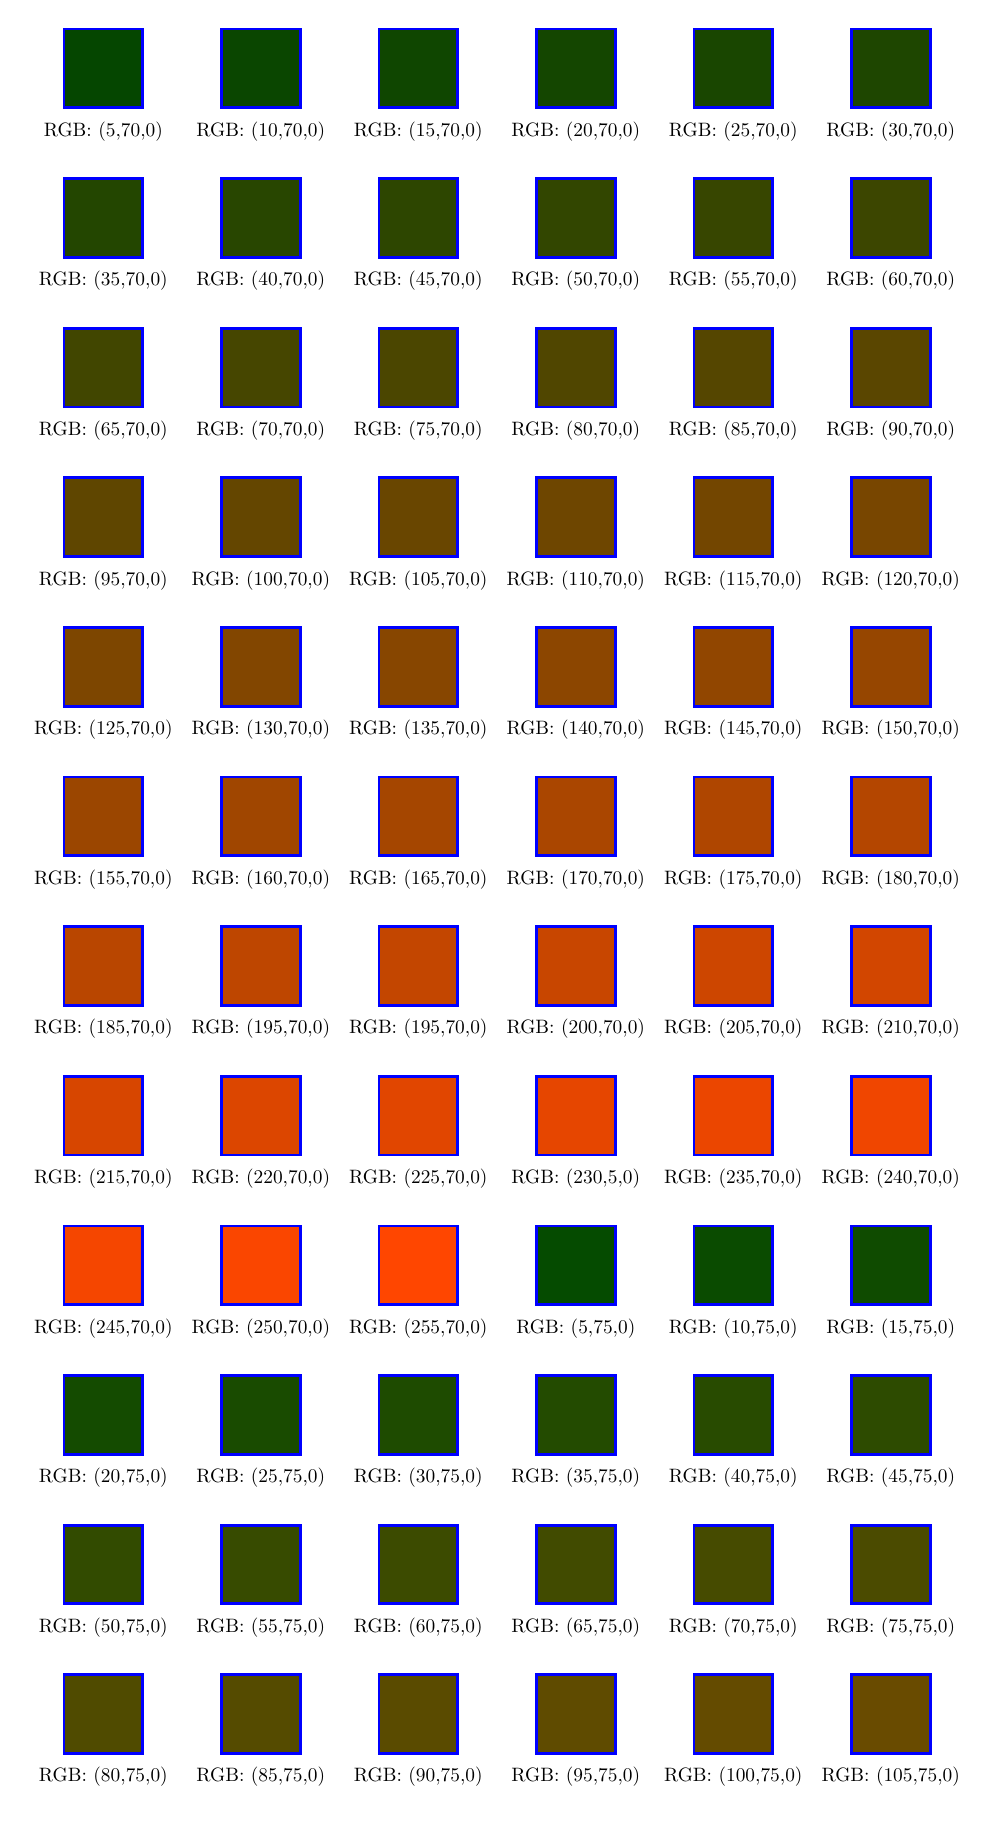
\begin{tikzpicture}

    \filldraw[draw=blue,line width=1,fill=colorR5G70B0]
    (0,0) rectangle (1,1);

    \node[scale=0.7] at (0.5,-0.3) {RGB: (5,70,0)};



    \begin{scope}[xshift=2cm]

      \filldraw[draw=blue,line width=1,fill=colorR10G70B0]
      (0,0) rectangle (1,1);

      \node[scale=0.7] at (0.5,-0.3) {RGB: (10,70,0)};

    \end{scope}



    \begin{scope}[xshift=4cm]

      \filldraw[draw=blue,line width=1,fill=colorR15G70B0]
      (0,0) rectangle (1,1);

      \node[scale=0.7] at (0.5,-0.3) {RGB: (15,70,0)};

    \end{scope}



    \begin{scope}[xshift=6cm]

      \filldraw[draw=blue,line width=1,fill=colorR20G70B0]
      (0,0) rectangle (1,1);

      \node[scale=0.7] at (0.5,-0.3) {RGB: (20,70,0)};

    \end{scope}



    \begin{scope}[xshift=8cm]

      \filldraw[draw=blue,line width=1,fill=colorR25G70B0]
      (0,0) rectangle (1,1);

      \node[scale=0.7] at (0.5,-0.3) {RGB: (25,70,0)};

    \end{scope}



    \begin{scope}[xshift=10cm]

      \filldraw[draw=blue,line width=1,fill=colorR30G70B0]
      (0,0) rectangle (1,1);

      \node[scale=0.7] at (0.5,-0.3) {RGB: (30,70,0)};

    \end{scope}







    \begin{scope}[yshift=-1.9cm]

      \filldraw[draw=blue,line width=1,fill=colorR35G70B0]
      (0,0) rectangle (1,1);

      \node[scale=0.7] at (0.5,-0.3) {RGB: (35,70,0)};

    \end{scope}



    \begin{scope}[xshift=2cm,yshift=-1.9cm]

      \filldraw[draw=blue,line width=1,fill=colorR40G70B0]
      (0,0) rectangle (1,1);

      \node[scale=0.7] at (0.5,-0.3) {RGB: (40,70,0)};

    \end{scope}



    \begin{scope}[xshift=4cm,yshift=-1.9cm]

      \filldraw[draw=blue,line width=1,fill=colorR45G70B0]
      (0,0) rectangle (1,1);

      \node[scale=0.7] at (0.5,-0.3) {RGB: (45,70,0)};

    \end{scope}



    \begin{scope}[xshift=6cm,yshift=-1.9cm]

      \filldraw[draw=blue,line width=1,fill=colorR50G70B0]
      (0,0) rectangle (1,1);

      \node[scale=0.7] at (0.5,-0.3) {RGB: (50,70,0)};

    \end{scope}



    \begin{scope}[xshift=8cm,yshift=-1.9cm]

      \filldraw[draw=blue,line width=1,fill=colorR55G70B0]
      (0,0) rectangle (1,1);

      \node[scale=0.7] at (0.5,-0.3) {RGB: (55,70,0)};

    \end{scope}



    \begin{scope}[xshift=10cm,yshift=-1.9cm]

      \filldraw[draw=blue,line width=1,fill=colorR60G70B0]
      (0,0) rectangle (1,1);

      \node[scale=0.7] at (0.5,-0.3) {RGB: (60,70,0)};

    \end{scope}







    \begin{scope}[yshift=-3.8cm]

      \filldraw[draw=blue,line width=1,fill=colorR65G70B0]
      (0,0) rectangle (1,1);

      \node[scale=0.7] at (0.5,-0.3) {RGB: (65,70,0)};

    \end{scope}



    \begin{scope}[xshift=2cm,yshift=-3.8cm]

      \filldraw[draw=blue,line width=1,fill=colorR70G70B0]
      (0,0) rectangle (1,1);

      \node[scale=0.7] at (0.5,-0.3) {RGB: (70,70,0)};

    \end{scope}



    \begin{scope}[xshift=4cm,yshift=-3.8cm]

      \filldraw[draw=blue,line width=1,fill=colorR75G70B0]
      (0,0) rectangle (1,1);

      \node[scale=0.7] at (0.5,-0.3) {RGB: (75,70,0)};

    \end{scope}



    \begin{scope}[xshift=6cm,yshift=-3.8cm]

      \filldraw[draw=blue,line width=1,fill=colorR80G70B0]
      (0,0) rectangle (1,1);

      \node[scale=0.7] at (0.5,-0.3) {RGB: (80,70,0)};

    \end{scope}



    \begin{scope}[xshift=8cm,yshift=-3.8cm]

      \filldraw[draw=blue,line width=1,fill=colorR85G70B0]
      (0,0) rectangle (1,1);

      \node[scale=0.7] at (0.5,-0.3) {RGB: (85,70,0)};

    \end{scope}



    \begin{scope}[xshift=10cm,yshift=-3.8cm]

      \filldraw[draw=blue,line width=1,fill=colorR90G70B0]
      (0,0) rectangle (1,1);

      \node[scale=0.7] at (0.5,-0.3) {RGB: (90,70,0)};

    \end{scope}







    \begin{scope}[yshift=-5.7cm]

      \filldraw[draw=blue,line width=1,fill=colorR95G70B0]
      (0,0) rectangle (1,1);

      \node[scale=0.7] at (0.5,-0.3) {RGB: (95,70,0)};

    \end{scope}



    \begin{scope}[xshift=2cm,yshift=-5.7cm]

      \filldraw[draw=blue,line width=1,fill=colorR100G70B0]
      (0,0) rectangle (1,1);

      \node[scale=0.7] at (0.5,-0.3) {RGB: (100,70,0)};

    \end{scope}



    \begin{scope}[xshift=4cm,yshift=-5.7cm]

      \filldraw[draw=blue,line width=1,fill=colorR105G70B0]
      (0,0) rectangle (1,1);

      \node[scale=0.7] at (0.5,-0.3) {RGB: (105,70,0)};

    \end{scope}



    \begin{scope}[xshift=6cm,yshift=-5.7cm]

      \filldraw[draw=blue,line width=1,fill=colorR110G70B0]
      (0,0) rectangle (1,1);

      \node[scale=0.7] at (0.5,-0.3) {RGB: (110,70,0)};

    \end{scope}



    \begin{scope}[xshift=8cm,yshift=-5.7cm]

      \filldraw[draw=blue,line width=1,fill=colorR115G70B0]
      (0,0) rectangle (1,1);

      \node[scale=0.7] at (0.5,-0.3) {RGB: (115,70,0)};

    \end{scope}



    \begin{scope}[xshift=10cm,yshift=-5.7cm]

      \filldraw[draw=blue,line width=1,fill=colorR120G70B0]
      (0,0) rectangle (1,1);

      \node[scale=0.7] at (0.5,-0.3) {RGB: (120,70,0)};

    \end{scope}







    \begin{scope}[yshift=-7.6cm]

      \filldraw[draw=blue,line width=1,fill=colorR125G70B0]
      (0,0) rectangle (1,1);

      \node[scale=0.7] at (0.5,-0.3) {RGB: (125,70,0)};

    \end{scope}



    \begin{scope}[xshift=2cm,yshift=-7.6cm]

      \filldraw[draw=blue,line width=1,fill=colorR130G70B0]
      (0,0) rectangle (1,1);

      \node[scale=0.7] at (0.5,-0.3) {RGB: (130,70,0)};

    \end{scope}



    \begin{scope}[xshift=4cm,yshift=-7.6cm]

      \filldraw[draw=blue,line width=1,fill=colorR135G70B0]
      (0,0) rectangle (1,1);

      \node[scale=0.7] at (0.5,-0.3) {RGB: (135,70,0)};

    \end{scope}



    \begin{scope}[xshift=6cm,yshift=-7.6cm]

      \filldraw[draw=blue,line width=1,fill=colorR140G70B0]
      (0,0) rectangle (1,1);

      \node[scale=0.7] at (0.5,-0.3) {RGB: (140,70,0)};

    \end{scope}



    \begin{scope}[xshift=8cm,yshift=-7.6cm]

      \filldraw[draw=blue,line width=1,fill=colorR145G70B0]
      (0,0) rectangle (1,1);

      \node[scale=0.7] at (0.5,-0.3) {RGB: (145,70,0)};

    \end{scope}



    \begin{scope}[xshift=10cm,yshift=-7.6cm]

      \filldraw[draw=blue,line width=1,fill=colorR150G70B0]
      (0,0) rectangle (1,1);

      \node[scale=0.7] at (0.5,-0.3) {RGB: (150,70,0)};

    \end{scope}







    \begin{scope}[yshift=-9.5cm]

      \filldraw[draw=blue,line width=1,fill=colorR155G70B0]
      (0,0) rectangle (1,1);

      \node[scale=0.7] at (0.5,-0.3) {RGB: (155,70,0)};

    \end{scope}



    \begin{scope}[xshift=2cm,yshift=-9.5cm]

      \filldraw[draw=blue,line width=1,fill=colorR160G70B0]
      (0,0) rectangle (1,1);

      \node[scale=0.7] at (0.5,-0.3) {RGB: (160,70,0)};

    \end{scope}



    \begin{scope}[xshift=4cm,yshift=-9.5cm]

      \filldraw[draw=blue,line width=1,fill=colorR165G70B0]
      (0,0) rectangle (1,1);

      \node[scale=0.7] at (0.5,-0.3) {RGB: (165,70,0)};

    \end{scope}



    \begin{scope}[xshift=6cm,yshift=-9.5cm]

      \filldraw[draw=blue,line width=1,fill=colorR170G70B0]
      (0,0) rectangle (1,1);

      \node[scale=0.7] at (0.5,-0.3) {RGB: (170,70,0)};

    \end{scope}



    \begin{scope}[xshift=8cm,yshift=-9.5cm]

      \filldraw[draw=blue,line width=1,fill=colorR175G70B0]
      (0,0) rectangle (1,1);

      \node[scale=0.7] at (0.5,-0.3) {RGB: (175,70,0)};

    \end{scope}



    \begin{scope}[xshift=10cm,yshift=-9.5cm]

      \filldraw[draw=blue,line width=1,fill=colorR180G70B0]
      (0,0) rectangle (1,1);

      \node[scale=0.7] at (0.5,-0.3) {RGB: (180,70,0)};

    \end{scope}







    \begin{scope}[yshift=-11.4cm]

      \filldraw[draw=blue,line width=1,fill=colorR185G70B0]
      (0,0) rectangle (1,1);

      \node[scale=0.7] at (0.5,-0.3) {RGB: (185,70,0)};

    \end{scope}



    \begin{scope}[xshift=2cm,yshift=-11.4cm]

      \filldraw[draw=blue,line width=1,fill=colorR190G70B0]
      (0,0) rectangle (1,1);

      \node[scale=0.7] at (0.5,-0.3) {RGB: (195,70,0)};

    \end{scope}



    \begin{scope}[xshift=4cm,yshift=-11.4cm]

      \filldraw[draw=blue,line width=1,fill=colorR195G70B0]
      (0,0) rectangle (1,1);

      \node[scale=0.7] at (0.5,-0.3) {RGB: (195,70,0)};

    \end{scope}



    \begin{scope}[xshift=6cm,yshift=-11.4cm]

      \filldraw[draw=blue,line width=1,fill=colorR200G70B0]
      (0,0) rectangle (1,1);

      \node[scale=0.7] at (0.5,-0.3) {RGB: (200,70,0)};

    \end{scope}



    \begin{scope}[xshift=8cm,yshift=-11.4cm]

      \filldraw[draw=blue,line width=1,fill=colorR205G70B0]
      (0,0) rectangle (1,1);

      \node[scale=0.7] at (0.5,-0.3) {RGB: (205,70,0)};

    \end{scope}



    \begin{scope}[xshift=10cm,yshift=-11.4cm]

      \filldraw[draw=blue,line width=1,fill=colorR210G70B0]
      (0,0) rectangle (1,1);

      \node[scale=0.7] at (0.5,-0.3) {RGB: (210,70,0)};

    \end{scope}







    \begin{scope}[yshift=-13.3cm]

      \filldraw[draw=blue,line width=1,fill=colorR215G70B0]
      (0,0) rectangle (1,1);

      \node[scale=0.7] at (0.5,-0.3) {RGB: (215,70,0)};

    \end{scope}



    \begin{scope}[xshift=2cm,yshift=-13.3cm]

      \filldraw[draw=blue,line width=1,fill=colorR220G70B0]
      (0,0) rectangle (1,1);

      \node[scale=0.7] at (0.5,-0.3) {RGB: (220,70,0)};

    \end{scope}



    \begin{scope}[xshift=4cm,yshift=-13.3cm]

      \filldraw[draw=blue,line width=1,fill=colorR225G70B0]
      (0,0) rectangle (1,1);

      \node[scale=0.7] at (0.5,-0.3) {RGB: (225,70,0)};

    \end{scope}



    \begin{scope}[xshift=6cm,yshift=-13.3cm]

      \filldraw[draw=blue,line width=1,fill=colorR230G70B0]
      (0,0) rectangle (1,1);

      \node[scale=0.7] at (0.5,-0.3) {RGB: (230,5,0)};

    \end{scope}



    \begin{scope}[xshift=8cm,yshift=-13.3cm]

      \filldraw[draw=blue,line width=1,fill=colorR235G70B0]
      (0,0) rectangle (1,1);

      \node[scale=0.7] at (0.5,-0.3) {RGB: (235,70,0)};

    \end{scope}



    \begin{scope}[xshift=10cm,yshift=-13.3cm]

      \filldraw[draw=blue,line width=1,fill=colorR240G70B0]
      (0,0) rectangle (1,1);

      \node[scale=0.7] at (0.5,-0.3) {RGB: (240,70,0)};

    \end{scope}







    \begin{scope}[yshift=-15.2cm]

      \filldraw[draw=blue,line width=1,fill=colorR245G70B0]
      (0,0) rectangle (1,1);

      \node[scale=0.7] at (0.5,-0.3) {RGB: (245,70,0)};

    \end{scope}



    \begin{scope}[xshift=2cm,yshift=-15.2cm]

      \filldraw[draw=blue,line width=1,fill=colorR250G70B0]
      (0,0) rectangle (1,1);

      \node[scale=0.7] at (0.5,-0.3) {RGB: (250,70,0)};

    \end{scope}



    \begin{scope}[xshift=4cm,yshift=-15.2cm]

      \filldraw[draw=blue,line width=1,fill=colorR255G70B0]
      (0,0) rectangle (1,1);

      \node[scale=0.7] at (0.5,-0.3) {RGB: (255,70,0)};

    \end{scope}



    \begin{scope}[xshift=6cm,yshift=-15.2cm]

      \filldraw[draw=blue,line width=1,fill=colorR5G75B0]
      (0,0) rectangle (1,1);

      \node[scale=0.7] at (0.5,-0.3) {RGB: (5,75,0)};

    \end{scope}



    \begin{scope}[xshift=8cm,yshift=-15.2cm]

      \filldraw[draw=blue,line width=1,fill=colorR10G75B0]
      (0,0) rectangle (1,1);

      \node[scale=0.7] at (0.5,-0.3) {RGB: (10,75,0)};

    \end{scope}



    \begin{scope}[xshift=10cm,yshift=-15.2cm]

      \filldraw[draw=blue,line width=1,fill=colorR15G75B0]
      (0,0) rectangle (1,1);

      \node[scale=0.7] at (0.5,-0.3) {RGB: (15,75,0)};

    \end{scope}







    \begin{scope}[yshift=-17.1cm]

      \filldraw[draw=blue,line width=1,fill=colorR20G75B0]
      (0,0) rectangle (1,1);

      \node[scale=0.7] at (0.5,-0.3) {RGB: (20,75,0)};

    \end{scope}



    \begin{scope}[xshift=2cm,yshift=-17.1cm]

      \filldraw[draw=blue,line width=1,fill=colorR25G75B0]
      (0,0) rectangle (1,1);

      \node[scale=0.7] at (0.5,-0.3) {RGB: (25,75,0)};

    \end{scope}



    \begin{scope}[xshift=4cm,yshift=-17.1cm]

      \filldraw[draw=blue,line width=1,fill=colorR30G75B0]
      (0,0) rectangle (1,1);

      \node[scale=0.7] at (0.5,-0.3) {RGB: (30,75,0)};

    \end{scope}



    \begin{scope}[xshift=6cm,yshift=-17.1cm]

      \filldraw[draw=blue,line width=1,fill=colorR35G75B0]
      (0,0) rectangle (1,1);

      \node[scale=0.7] at (0.5,-0.3) {RGB: (35,75,0)};

    \end{scope}



    \begin{scope}[xshift=8cm,yshift=-17.1cm]

      \filldraw[draw=blue,line width=1,fill=colorR40G75B0]
      (0,0) rectangle (1,1);

      \node[scale=0.7] at (0.5,-0.3) {RGB: (40,75,0)};

    \end{scope}



    \begin{scope}[xshift=10cm,yshift=-17.1cm]

      \filldraw[draw=blue,line width=1,fill=colorR45G75B0]
      (0,0) rectangle (1,1);

      \node[scale=0.7] at (0.5,-0.3) {RGB: (45,75,0)};

    \end{scope}







    \begin{scope}[yshift=-19cm]

      \filldraw[draw=blue,line width=1,fill=colorR50G75B0]
      (0,0) rectangle (1,1);

      \node[scale=0.7] at (0.5,-0.3) {RGB: (50,75,0)};

    \end{scope}



    \begin{scope}[xshift=2cm,yshift=-19cm]

      \filldraw[draw=blue,line width=1,fill=colorR55G75B0]
      (0,0) rectangle (1,1);

      \node[scale=0.7] at (0.5,-0.3) {RGB: (55,75,0)};

    \end{scope}



    \begin{scope}[xshift=4cm,yshift=-19cm]

      \filldraw[draw=blue,line width=1,fill=colorR60G75B0]
      (0,0) rectangle (1,1);

      \node[scale=0.7] at (0.5,-0.3) {RGB: (60,75,0)};

    \end{scope}



    \begin{scope}[xshift=6cm,yshift=-19cm]

      \filldraw[draw=blue,line width=1,fill=colorR65G75B0]
      (0,0) rectangle (1,1);

      \node[scale=0.7] at (0.5,-0.3) {RGB: (65,75,0)};

    \end{scope}



    \begin{scope}[xshift=8cm,yshift=-19cm]

      \filldraw[draw=blue,line width=1,fill=colorR70G75B0]
      (0,0) rectangle (1,1);

      \node[scale=0.7] at (0.5,-0.3) {RGB: (70,75,0)};

    \end{scope}



    \begin{scope}[xshift=10cm,yshift=-19cm]

      \filldraw[draw=blue,line width=1,fill=colorR75G75B0]
      (0,0) rectangle (1,1);

      \node[scale=0.7] at (0.5,-0.3) {RGB: (75,75,0)};

    \end{scope}







    \begin{scope}[yshift=-20.9cm]

      \filldraw[draw=blue,line width=1,fill=colorR80G75B0]
      (0,0) rectangle (1,1);

      \node[scale=0.7] at (0.5,-0.3) {RGB: (80,75,0)};

    \end{scope}



    \begin{scope}[xshift=2cm,yshift=-20.9cm]

      \filldraw[draw=blue,line width=1,fill=colorR85G75B0]
      (0,0) rectangle (1,1);

      \node[scale=0.7] at (0.5,-0.3) {RGB: (85,75,0)};

    \end{scope}



    \begin{scope}[xshift=4cm,yshift=-20.9cm]

      \filldraw[draw=blue,line width=1,fill=colorR90G75B0]
      (0,0) rectangle (1,1);

      \node[scale=0.7] at (0.5,-0.3) {RGB: (90,75,0)};

    \end{scope}



    \begin{scope}[xshift=6cm,yshift=-20.9cm]

      \filldraw[draw=blue,line width=1,fill=colorR95G75B0]
      (0,0) rectangle (1,1);

      \node[scale=0.7] at (0.5,-0.3) {RGB: (95,75,0)};

    \end{scope}



    \begin{scope}[xshift=8cm,yshift=-20.9cm]

      \filldraw[draw=blue,line width=1,fill=colorR100G75B0]
      (0,0) rectangle (1,1);

      \node[scale=0.7] at (0.5,-0.3) {RGB: (100,75,0)};

    \end{scope}



    \begin{scope}[xshift=10cm,yshift=-20.9cm]

      \filldraw[draw=blue,line width=1,fill=colorR105G75B0]
      (0,0) rectangle (1,1);

      \node[scale=0.7] at (0.5,-0.3) {RGB: (105,75,0)};

    \end{scope}

  \end{tikzpicture}

  \caption{Mixed colors in~RGB system: $(5,70,0)$--$(255,70,0)$,
    $(5,75,0)$--$(105,75,0)$}



  \label{fig:Mixed-colors-Part-01}

\end{figure}
% ##################





% ##################
\begin{figure}

  \centering


  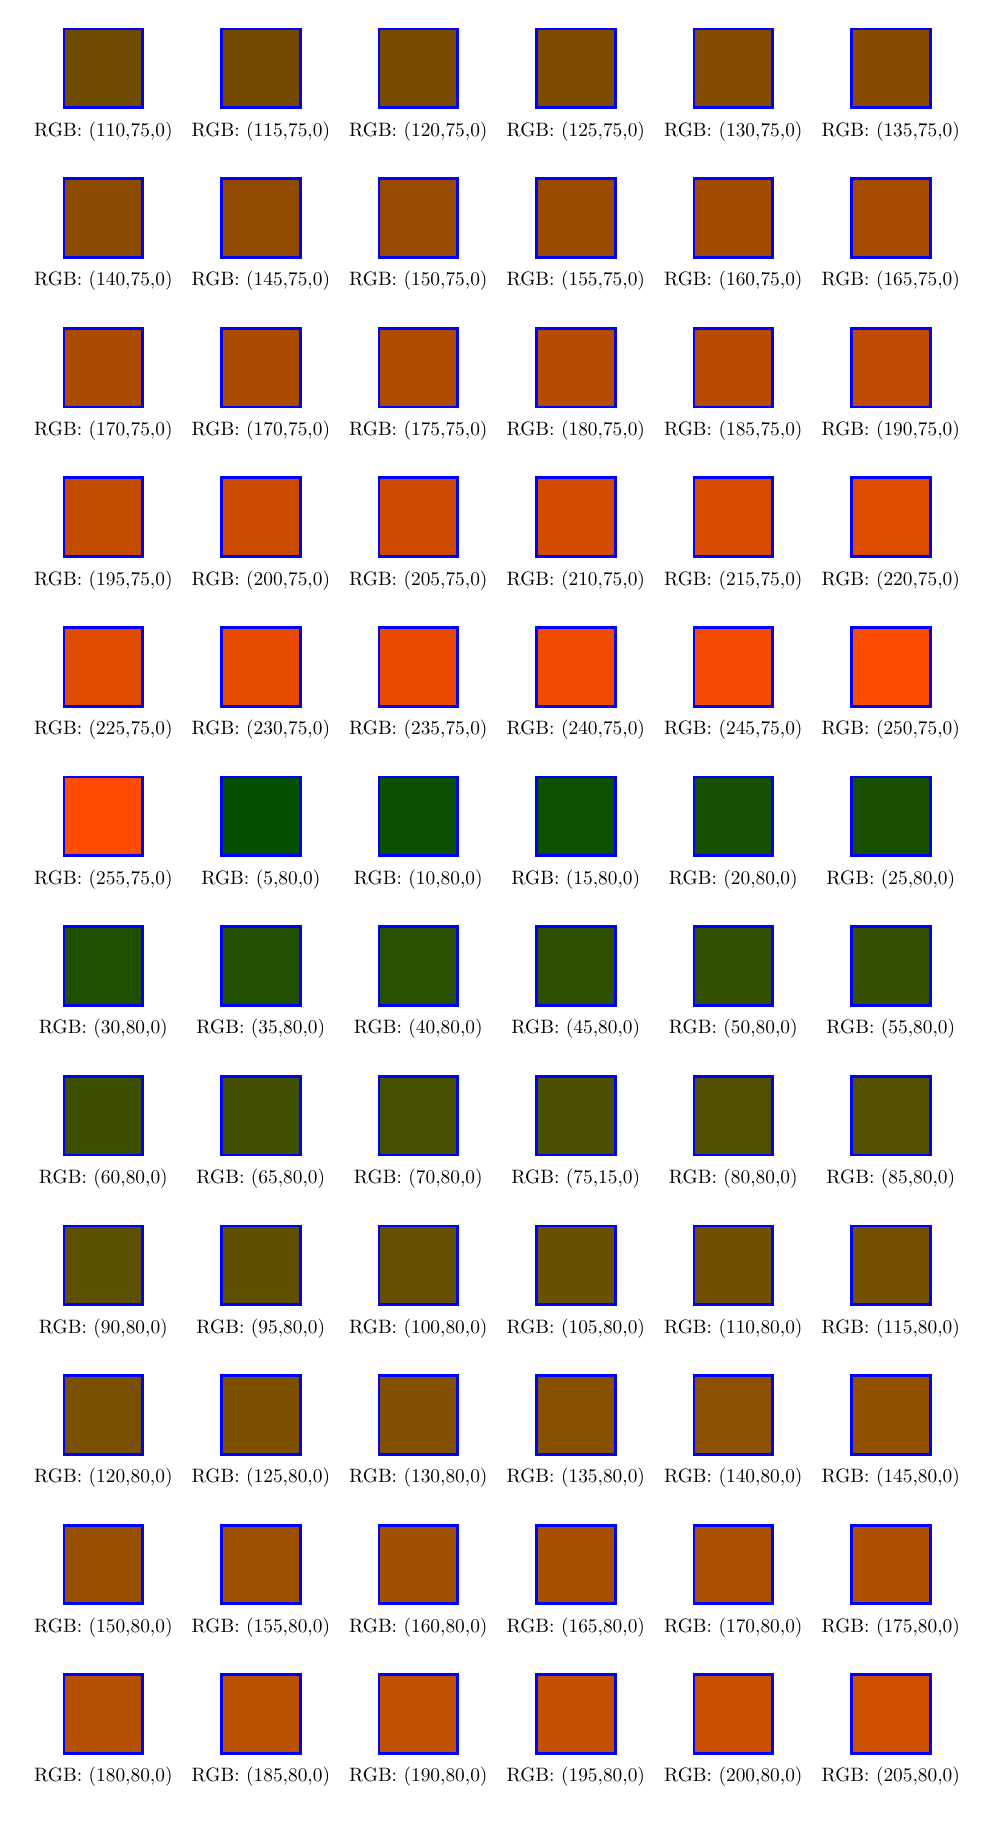
\begin{tikzpicture}

    \filldraw[draw=blue,line width=1,fill=colorR110G75B0]
    (0,0) rectangle (1,1);

    \node[scale=0.7] at (0.5,-0.3) {RGB: (110,75,0)};



    \begin{scope}[xshift=2cm]

      \filldraw[draw=blue,line width=1,fill=colorR115G75B0]
      (0,0) rectangle (1,1);

      \node[scale=0.7] at (0.5,-0.3) {RGB: (115,75,0)};

    \end{scope}



    \begin{scope}[xshift=4cm]

      \filldraw[draw=blue,line width=1,fill=colorR120G75B0]
      (0,0) rectangle (1,1);

      \node[scale=0.7] at (0.5,-0.3) {RGB: (120,75,0)};

    \end{scope}



    \begin{scope}[xshift=6cm]

      \filldraw[draw=blue,line width=1,fill=colorR125G75B0]
      (0,0) rectangle (1,1);

      \node[scale=0.7] at (0.5,-0.3) {RGB: (125,75,0)};

    \end{scope}



    \begin{scope}[xshift=8cm]

      \filldraw[draw=blue,line width=1,fill=colorR130G75B0]
      (0,0) rectangle (1,1);

      \node[scale=0.7] at (0.5,-0.3) {RGB: (130,75,0)};

    \end{scope}



    \begin{scope}[xshift=10cm]

      \filldraw[draw=blue,line width=1,fill=colorR135G75B0]
      (0,0) rectangle (1,1);

      \node[scale=0.7] at (0.5,-0.3) {RGB: (135,75,0)};

    \end{scope}







    \begin{scope}[yshift=-1.9cm]

      \filldraw[draw=blue,line width=1,fill=colorR140G75B0]
      (0,0) rectangle (1,1);

      \node[scale=0.7] at (0.5,-0.3) {RGB: (140,75,0)};

    \end{scope}



    \begin{scope}[xshift=2cm,yshift=-1.9cm]

      \filldraw[draw=blue,line width=1,fill=colorR145G75B0]
      (0,0) rectangle (1,1);

      \node[scale=0.7] at (0.5,-0.3) {RGB: (145,75,0)};

    \end{scope}



    \begin{scope}[xshift=4cm,yshift=-1.9cm]

      \filldraw[draw=blue,line width=1,fill=colorR150G75B0]
      (0,0) rectangle (1,1);

      \node[scale=0.7] at (0.5,-0.3) {RGB: (150,75,0)};

    \end{scope}



    \begin{scope}[xshift=6cm,yshift=-1.9cm]

      \filldraw[draw=blue,line width=1,fill=colorR155G75B0]
      (0,0) rectangle (1,1);

      \node[scale=0.7] at (0.5,-0.3) {RGB: (155,75,0)};

    \end{scope}



    \begin{scope}[xshift=8cm,yshift=-1.9cm]

      \filldraw[draw=blue,line width=1,fill=colorR160G75B0]
      (0,0) rectangle (1,1);

      \node[scale=0.7] at (0.5,-0.3) {RGB: (160,75,0)};

    \end{scope}



    \begin{scope}[xshift=10cm,yshift=-1.9cm]

      \filldraw[draw=blue,line width=1,fill=colorR165G75B0]
      (0,0) rectangle (1,1);

      \node[scale=0.7] at (0.5,-0.3) {RGB: (165,75,0)};

    \end{scope}







    \begin{scope}[yshift=-3.8cm]

      \filldraw[draw=blue,line width=1,fill=colorR170G75B0]
      (0,0) rectangle (1,1);

      \node[scale=0.7] at (0.5,-0.3) {RGB: (170,75,0)};

    \end{scope}



    \begin{scope}[xshift=2cm,yshift=-3.8cm]

      \filldraw[draw=blue,line width=1,fill=colorR170G75B0]
      (0,0) rectangle (1,1);

      \node[scale=0.7] at (0.5,-0.3) {RGB: (170,75,0)};

    \end{scope}



    \begin{scope}[xshift=4cm,yshift=-3.8cm]

      \filldraw[draw=blue,line width=1,fill=colorR175G75B0]
      (0,0) rectangle (1,1);

      \node[scale=0.7] at (0.5,-0.3) {RGB: (175,75,0)};

    \end{scope}



    \begin{scope}[xshift=6cm,yshift=-3.8cm]

      \filldraw[draw=blue,line width=1,fill=colorR180G75B0]
      (0,0) rectangle (1,1);

      \node[scale=0.7] at (0.5,-0.3) {RGB: (180,75,0)};

    \end{scope}



    \begin{scope}[xshift=8cm,yshift=-3.8cm]

      \filldraw[draw=blue,line width=1,fill=colorR185G75B0]
      (0,0) rectangle (1,1);

      \node[scale=0.7] at (0.5,-0.3) {RGB: (185,75,0)};

    \end{scope}



    \begin{scope}[xshift=10cm,yshift=-3.8cm]

      \filldraw[draw=blue,line width=1,fill=colorR190G75B0]
      (0,0) rectangle (1,1);

      \node[scale=0.7] at (0.5,-0.3) {RGB: (190,75,0)};

    \end{scope}







    \begin{scope}[yshift=-5.7cm]

      \filldraw[draw=blue,line width=1,fill=colorR195G75B0]
      (0,0) rectangle (1,1);

      \node[scale=0.7] at (0.5,-0.3) {RGB: (195,75,0)};

    \end{scope}



    \begin{scope}[xshift=2cm,yshift=-5.7cm]

      \filldraw[draw=blue,line width=1,fill=colorR200G75B0]
      (0,0) rectangle (1,1);

      \node[scale=0.7] at (0.5,-0.3) {RGB: (200,75,0)};

    \end{scope}



    \begin{scope}[xshift=4cm,yshift=-5.7cm]

      \filldraw[draw=blue,line width=1,fill=colorR205G75B0]
      (0,0) rectangle (1,1);

      \node[scale=0.7] at (0.5,-0.3) {RGB: (205,75,0)};

    \end{scope}



    \begin{scope}[xshift=6cm,yshift=-5.7cm]

      \filldraw[draw=blue,line width=1,fill=colorR210G75B0]
      (0,0) rectangle (1,1);

      \node[scale=0.7] at (0.5,-0.3) {RGB: (210,75,0)};

    \end{scope}



    \begin{scope}[xshift=8cm,yshift=-5.7cm]

      \filldraw[draw=blue,line width=1,fill=colorR215G75B0]
      (0,0) rectangle (1,1);

      \node[scale=0.7] at (0.5,-0.3) {RGB: (215,75,0)};

    \end{scope}



    \begin{scope}[xshift=10cm,yshift=-5.7cm]

      \filldraw[draw=blue,line width=1,fill=colorR220G75B0]
      (0,0) rectangle (1,1);

      \node[scale=0.7] at (0.5,-0.3) {RGB: (220,75,0)};

    \end{scope}







    \begin{scope}[yshift=-7.6cm]

      \filldraw[draw=blue,line width=1,fill=colorR225G75B0]
      (0,0) rectangle (1,1);

      \node[scale=0.7] at (0.5,-0.3) {RGB: (225,75,0)};

    \end{scope}



    \begin{scope}[xshift=2cm,yshift=-7.6cm]

      \filldraw[draw=blue,line width=1,fill=colorR230G75B0]
      (0,0) rectangle (1,1);

      \node[scale=0.7] at (0.5,-0.3) {RGB: (230,75,0)};

    \end{scope}



    \begin{scope}[xshift=4cm,yshift=-7.6cm]

      \filldraw[draw=blue,line width=1,fill=colorR235G75B0]
      (0,0) rectangle (1,1);

      \node[scale=0.7] at (0.5,-0.3) {RGB: (235,75,0)};

    \end{scope}



    \begin{scope}[xshift=6cm,yshift=-7.6cm]

      \filldraw[draw=blue,line width=1,fill=colorR240G75B0]
      (0,0) rectangle (1,1);

      \node[scale=0.7] at (0.5,-0.3) {RGB: (240,75,0)};

    \end{scope}



    \begin{scope}[xshift=8cm,yshift=-7.6cm]

      \filldraw[draw=blue,line width=1,fill=colorR245G75B0]
      (0,0) rectangle (1,1);

      \node[scale=0.7] at (0.5,-0.3) {RGB: (245,75,0)};

    \end{scope}



    \begin{scope}[xshift=10cm,yshift=-7.6cm]

      \filldraw[draw=blue,line width=1,fill=colorR250G75B0]
      (0,0) rectangle (1,1);

      \node[scale=0.7] at (0.5,-0.3) {RGB: (250,75,0)};

    \end{scope}







    \begin{scope}[yshift=-9.5cm]

      \filldraw[draw=blue,line width=1,fill=colorR255G75B0]
      (0,0) rectangle (1,1);

      \node[scale=0.7] at (0.5,-0.3) {RGB: (255,75,0)};

    \end{scope}



    \begin{scope}[xshift=2cm,yshift=-9.5cm]

      \filldraw[draw=blue,line width=1,fill=colorR5G80B0]
      (0,0) rectangle (1,1);

      \node[scale=0.7] at (0.5,-0.3) {RGB: (5,80,0)};

    \end{scope}



    \begin{scope}[xshift=4cm,yshift=-9.5cm]

      \filldraw[draw=blue,line width=1,fill=colorR10G80B0]
      (0,0) rectangle (1,1);

      \node[scale=0.7] at (0.5,-0.3) {RGB: (10,80,0)};

    \end{scope}



    \begin{scope}[xshift=6cm,yshift=-9.5cm]

      \filldraw[draw=blue,line width=1,fill=colorR15G80B0]
      (0,0) rectangle (1,1);

      \node[scale=0.7] at (0.5,-0.3) {RGB: (15,80,0)};

    \end{scope}



    \begin{scope}[xshift=8cm,yshift=-9.5cm]

      \filldraw[draw=blue,line width=1,fill=colorR20G80B0]
      (0,0) rectangle (1,1);

      \node[scale=0.7] at (0.5,-0.3) {RGB: (20,80,0)};

    \end{scope}



    \begin{scope}[xshift=10cm,yshift=-9.5cm]

      \filldraw[draw=blue,line width=1,fill=colorR25G80B0]
      (0,0) rectangle (1,1);

      \node[scale=0.7] at (0.5,-0.3) {RGB: (25,80,0)};

    \end{scope}







    \begin{scope}[yshift=-11.4cm]

      \filldraw[draw=blue,line width=1,fill=colorR30G80B0]
      (0,0) rectangle (1,1);

      \node[scale=0.7] at (0.5,-0.3) {RGB: (30,80,0)};

    \end{scope}



    \begin{scope}[xshift=2cm,yshift=-11.4cm]

      \filldraw[draw=blue,line width=1,fill=colorR35G80B0]
      (0,0) rectangle (1,1);

      \node[scale=0.7] at (0.5,-0.3) {RGB: (35,80,0)};

    \end{scope}



    \begin{scope}[xshift=4cm,yshift=-11.4cm]

      \filldraw[draw=blue,line width=1,fill=colorR40G80B0]
      (0,0) rectangle (1,1);

      \node[scale=0.7] at (0.5,-0.3) {RGB: (40,80,0)};

    \end{scope}



    \begin{scope}[xshift=6cm,yshift=-11.4cm]

      \filldraw[draw=blue,line width=1,fill=colorR45G80B0]
      (0,0) rectangle (1,1);

      \node[scale=0.7] at (0.5,-0.3) {RGB: (45,80,0)};

    \end{scope}



    \begin{scope}[xshift=8cm,yshift=-11.4cm]

      \filldraw[draw=blue,line width=1,fill=colorR50G80B0]
      (0,0) rectangle (1,1);

      \node[scale=0.7] at (0.5,-0.3) {RGB: (50,80,0)};

    \end{scope}



    \begin{scope}[xshift=10cm,yshift=-11.4cm]

      \filldraw[draw=blue,line width=1,fill=colorR55G80B0]
      (0,0) rectangle (1,1);

      \node[scale=0.7] at (0.5,-0.3) {RGB: (55,80,0)};

    \end{scope}







    \begin{scope}[yshift=-13.3cm]

      \filldraw[draw=blue,line width=1,fill=colorR60G80B0]
      (0,0) rectangle (1,1);

      \node[scale=0.7] at (0.5,-0.3) {RGB: (60,80,0)};

    \end{scope}



    \begin{scope}[xshift=2cm,yshift=-13.3cm]

      \filldraw[draw=blue,line width=1,fill=colorR65G80B0]
      (0,0) rectangle (1,1);

      \node[scale=0.7] at (0.5,-0.3) {RGB: (65,80,0)};

    \end{scope}



    \begin{scope}[xshift=4cm,yshift=-13.3cm]

      \filldraw[draw=blue,line width=1,fill=colorR70G80B0]
      (0,0) rectangle (1,1);

      \node[scale=0.7] at (0.5,-0.3) {RGB: (70,80,0)};

    \end{scope}



    \begin{scope}[xshift=6cm,yshift=-13.3cm]

      \filldraw[draw=blue,line width=1,fill=colorR75G80B0]
      (0,0) rectangle (1,1);

      \node[scale=0.7] at (0.5,-0.3) {RGB: (75,15,0)};

    \end{scope}



    \begin{scope}[xshift=8cm,yshift=-13.3cm]

      \filldraw[draw=blue,line width=1,fill=colorR80G80B0]
      (0,0) rectangle (1,1);

      \node[scale=0.7] at (0.5,-0.3) {RGB: (80,80,0)};

    \end{scope}



    \begin{scope}[xshift=10cm,yshift=-13.3cm]

      \filldraw[draw=blue,line width=1,fill=colorR85G80B0]
      (0,0) rectangle (1,1);

      \node[scale=0.7] at (0.5,-0.3) {RGB: (85,80,0)};

    \end{scope}







    \begin{scope}[yshift=-15.2cm]

      \filldraw[draw=blue,line width=1,fill=colorR90G80B0]
      (0,0) rectangle (1,1);

      \node[scale=0.7] at (0.5,-0.3) {RGB: (90,80,0)};

    \end{scope}



    \begin{scope}[xshift=2cm,yshift=-15.2cm]

      \filldraw[draw=blue,line width=1,fill=colorR95G80B0]
      (0,0) rectangle (1,1);

      \node[scale=0.7] at (0.5,-0.3) {RGB: (95,80,0)};

    \end{scope}



    \begin{scope}[xshift=4cm,yshift=-15.2cm]

      \filldraw[draw=blue,line width=1,fill=colorR100G80B0]
      (0,0) rectangle (1,1);

      \node[scale=0.7] at (0.5,-0.3) {RGB: (100,80,0)};

    \end{scope}



    \begin{scope}[xshift=6cm,yshift=-15.2cm]

      \filldraw[draw=blue,line width=1,fill=colorR105G80B0]
      (0,0) rectangle (1,1);

      \node[scale=0.7] at (0.5,-0.3) {RGB: (105,80,0)};

    \end{scope}



    \begin{scope}[xshift=8cm,yshift=-15.2cm]

      \filldraw[draw=blue,line width=1,fill=colorR110G80B0]
      (0,0) rectangle (1,1);

      \node[scale=0.7] at (0.5,-0.3) {RGB: (110,80,0)};

    \end{scope}



    \begin{scope}[xshift=10cm,yshift=-15.2cm]

      \filldraw[draw=blue,line width=1,fill=colorR115G80B0]
      (0,0) rectangle (1,1);

      \node[scale=0.7] at (0.5,-0.3) {RGB: (115,80,0)};

    \end{scope}







    \begin{scope}[yshift=-17.1cm]

      \filldraw[draw=blue,line width=1,fill=colorR120G80B0]
      (0,0) rectangle (1,1);

      \node[scale=0.7] at (0.5,-0.3) {RGB: (120,80,0)};

    \end{scope}



    \begin{scope}[xshift=2cm,yshift=-17.1cm]

      \filldraw[draw=blue,line width=1,fill=colorR125G80B0]
      (0,0) rectangle (1,1);

      \node[scale=0.7] at (0.5,-0.3) {RGB: (125,80,0)};

    \end{scope}



    \begin{scope}[xshift=4cm,yshift=-17.1cm]

      \filldraw[draw=blue,line width=1,fill=colorR130G80B0]
      (0,0) rectangle (1,1);

      \node[scale=0.7] at (0.5,-0.3) {RGB: (130,80,0)};

    \end{scope}



    \begin{scope}[xshift=6cm,yshift=-17.1cm]

      \filldraw[draw=blue,line width=1,fill=colorR135G80B0]
      (0,0) rectangle (1,1);

      \node[scale=0.7] at (0.5,-0.3) {RGB: (135,80,0)};

    \end{scope}



    \begin{scope}[xshift=8cm,yshift=-17.1cm]

      \filldraw[draw=blue,line width=1,fill=colorR140G80B0]
      (0,0) rectangle (1,1);

      \node[scale=0.7] at (0.5,-0.3) {RGB: (140,80,0)};

    \end{scope}



    \begin{scope}[xshift=10cm,yshift=-17.1cm]

      \filldraw[draw=blue,line width=1,fill=colorR145G80B0]
      (0,0) rectangle (1,1);

      \node[scale=0.7] at (0.5,-0.3) {RGB: (145,80,0)};

    \end{scope}







    \begin{scope}[yshift=-19cm]

      \filldraw[draw=blue,line width=1,fill=colorR150G80B0]
      (0,0) rectangle (1,1);

      \node[scale=0.7] at (0.5,-0.3) {RGB: (150,80,0)};

    \end{scope}



    \begin{scope}[xshift=2cm,yshift=-19cm]

      \filldraw[draw=blue,line width=1,fill=colorR155G80B0]
      (0,0) rectangle (1,1);

      \node[scale=0.7] at (0.5,-0.3) {RGB: (155,80,0)};

    \end{scope}



    \begin{scope}[xshift=4cm,yshift=-19cm]

      \filldraw[draw=blue,line width=1,fill=colorR160G80B0]
      (0,0) rectangle (1,1);

      \node[scale=0.7] at (0.5,-0.3) {RGB: (160,80,0)};

    \end{scope}



    \begin{scope}[xshift=6cm,yshift=-19cm]

      \filldraw[draw=blue,line width=1,fill=colorR165G80B0]
      (0,0) rectangle (1,1);

      \node[scale=0.7] at (0.5,-0.3) {RGB: (165,80,0)};

    \end{scope}



    \begin{scope}[xshift=8cm,yshift=-19cm]

      \filldraw[draw=blue,line width=1,fill=colorR170G80B0]
      (0,0) rectangle (1,1);

      \node[scale=0.7] at (0.5,-0.3) {RGB: (170,80,0)};

    \end{scope}



    \begin{scope}[xshift=10cm,yshift=-19cm]

      \filldraw[draw=blue,line width=1,fill=colorR175G80B0]
      (0,0) rectangle (1,1);

      \node[scale=0.7] at (0.5,-0.3) {RGB: (175,80,0)};

    \end{scope}







    \begin{scope}[yshift=-20.9cm]

      \filldraw[draw=blue,line width=1,fill=colorR180G80B0]
      (0,0) rectangle (1,1);

      \node[scale=0.7] at (0.5,-0.3) {RGB: (180,80,0)};

    \end{scope}



    \begin{scope}[xshift=2cm,yshift=-20.9cm]

      \filldraw[draw=blue,line width=1,fill=colorR185G80B0]
      (0,0) rectangle (1,1);

      \node[scale=0.7] at (0.5,-0.3) {RGB: (185,80,0)};

    \end{scope}



    \begin{scope}[xshift=4cm,yshift=-20.9cm]

      \filldraw[draw=blue,line width=1,fill=colorR190G80B0]
      (0,0) rectangle (1,1);

      \node[scale=0.7] at (0.5,-0.3) {RGB: (190,80,0)};

    \end{scope}



    \begin{scope}[xshift=6cm,yshift=-20.9cm]

      \filldraw[draw=blue,line width=1,fill=colorR195G80B0]
      (0,0) rectangle (1,1);

      \node[scale=0.7] at (0.5,-0.3) {RGB: (195,80,0)};

    \end{scope}



    \begin{scope}[xshift=8cm,yshift=-20.9cm]

      \filldraw[draw=blue,line width=1,fill=colorR200G80B0]
      (0,0) rectangle (1,1);

      \node[scale=0.7] at (0.5,-0.3) {RGB: (200,80,0)};

    \end{scope}



    \begin{scope}[xshift=10cm,yshift=-20.9cm]

      \filldraw[draw=blue,line width=1,fill=colorR205G80B0]
      (0,0) rectangle (1,1);

      \node[scale=0.7] at (0.5,-0.3) {RGB: (205,80,0)};

    \end{scope}

  \end{tikzpicture}

  \caption{Mixed colors in~RGB system: $(110,75,0)$--$(255,75,0)$,
    $(5,80,0)$--$(205,80,0)$}



  \label{fig:Mixed-colors-Part-02}

\end{figure}
% ##################





% ##################
\begin{figure}

  \centering


  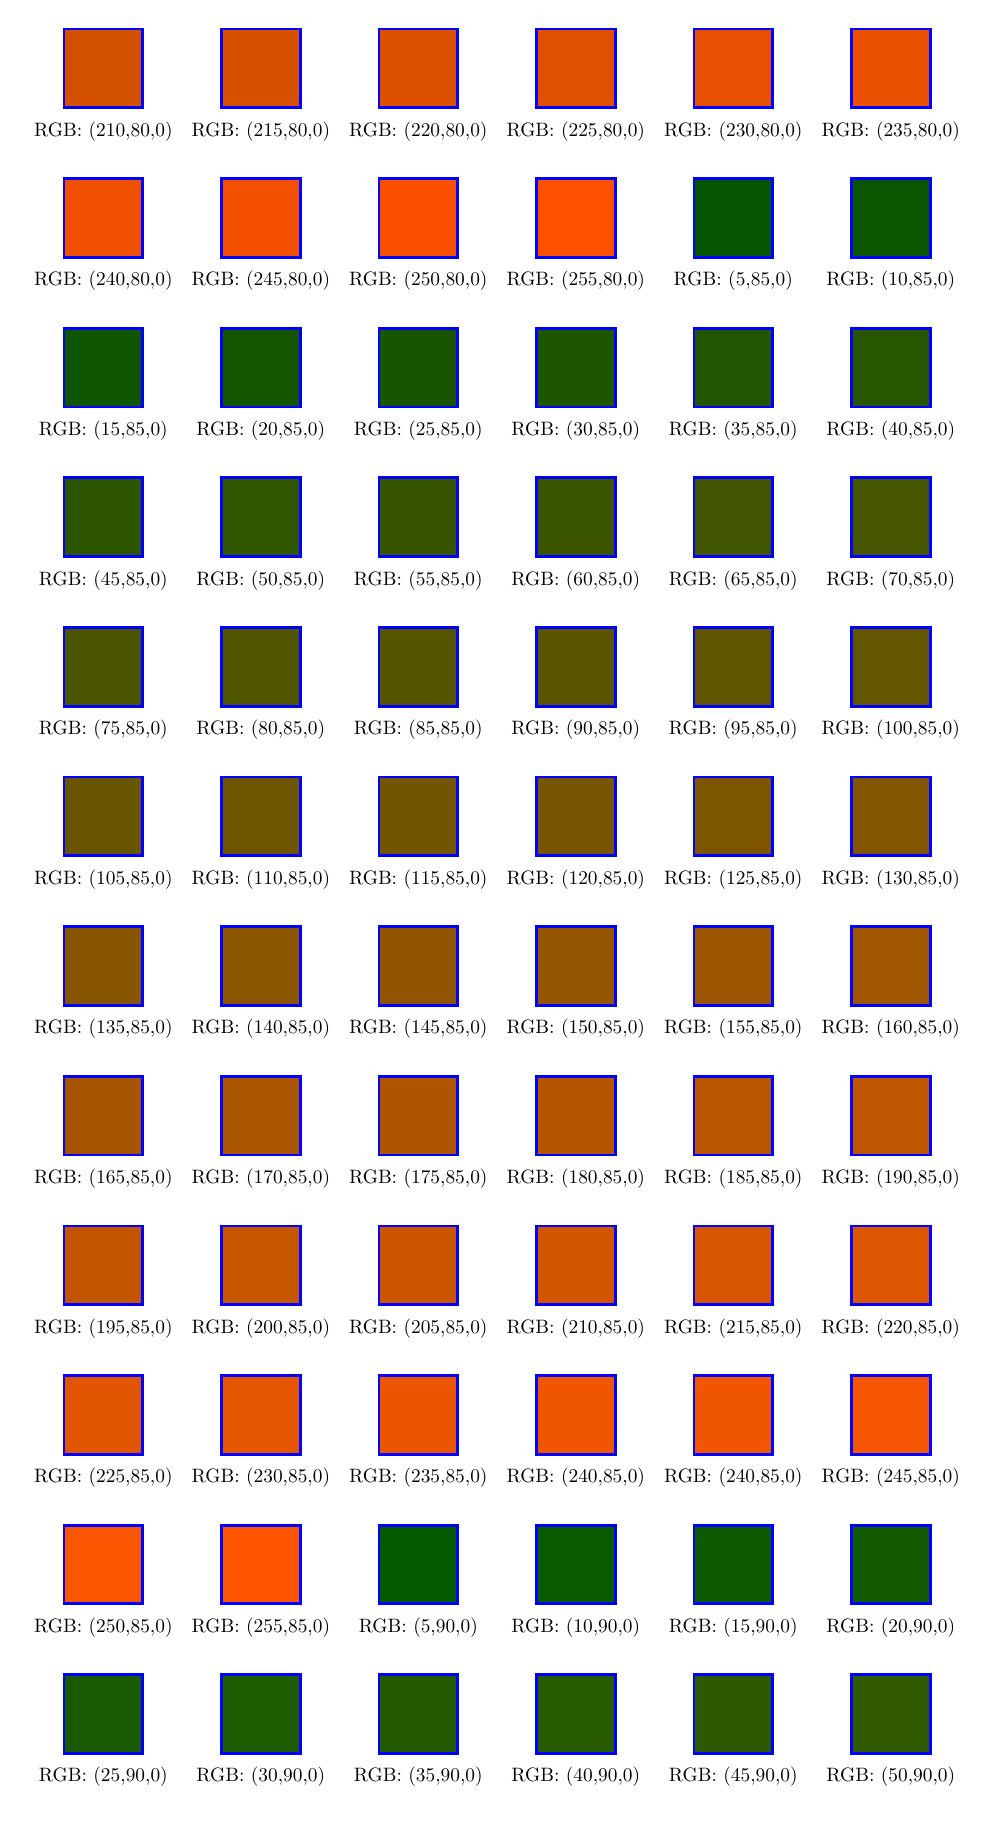
\begin{tikzpicture}

    \filldraw[draw=blue,line width=1,fill=colorR210G80B0]
    (0,0) rectangle (1,1);

    \node[scale=0.7] at (0.5,-0.3) {RGB: (210,80,0)};



    \begin{scope}[xshift=2cm]

      \filldraw[draw=blue,line width=1,fill=colorR215G80B0]
      (0,0) rectangle (1,1);

      \node[scale=0.7] at (0.5,-0.3) {RGB: (215,80,0)};

    \end{scope}



    \begin{scope}[xshift=4cm]

      \filldraw[draw=blue,line width=1,fill=colorR220G80B0]
      (0,0) rectangle (1,1);

      \node[scale=0.7] at (0.5,-0.3) {RGB: (220,80,0)};

    \end{scope}



    \begin{scope}[xshift=6cm]

      \filldraw[draw=blue,line width=1,fill=colorR225G80B0]
      (0,0) rectangle (1,1);

      \node[scale=0.7] at (0.5,-0.3) {RGB: (225,80,0)};

    \end{scope}



    \begin{scope}[xshift=8cm]

      \filldraw[draw=blue,line width=1,fill=colorR230G80B0]
      (0,0) rectangle (1,1);

      \node[scale=0.7] at (0.5,-0.3) {RGB: (230,80,0)};

    \end{scope}



    \begin{scope}[xshift=10cm]

      \filldraw[draw=blue,line width=1,fill=colorR235G80B0]
      (0,0) rectangle (1,1);

      \node[scale=0.7] at (0.5,-0.3) {RGB: (235,80,0)};

    \end{scope}







    \begin{scope}[yshift=-1.9cm]

      \filldraw[draw=blue,line width=1,fill=colorR240G80B0]
      (0,0) rectangle (1,1);

      \node[scale=0.7] at (0.5,-0.3) {RGB: (240,80,0)};

    \end{scope}



    \begin{scope}[xshift=2cm,yshift=-1.9cm]

      \filldraw[draw=blue,line width=1,fill=colorR245G80B0]
      (0,0) rectangle (1,1);

      \node[scale=0.7] at (0.5,-0.3) {RGB: (245,80,0)};

    \end{scope}



    \begin{scope}[xshift=4cm,yshift=-1.9cm]

      \filldraw[draw=blue,line width=1,fill=colorR250G80B0]
      (0,0) rectangle (1,1);

      \node[scale=0.7] at (0.5,-0.3) {RGB: (250,80,0)};

    \end{scope}



    \begin{scope}[xshift=6cm,yshift=-1.9cm]

      \filldraw[draw=blue,line width=1,fill=colorR255G80B0]
      (0,0) rectangle (1,1);

      \node[scale=0.7] at (0.5,-0.3) {RGB: (255,80,0)};

    \end{scope}



    \begin{scope}[xshift=8cm,yshift=-1.9cm]

      \filldraw[draw=blue,line width=1,fill=colorR5G85B0]
      (0,0) rectangle (1,1);

      \node[scale=0.7] at (0.5,-0.3) {RGB: (5,85,0)};

    \end{scope}



    \begin{scope}[xshift=10cm,yshift=-1.9cm]

      \filldraw[draw=blue,line width=1,fill=colorR10G85B0]
      (0,0) rectangle (1,1);

      \node[scale=0.7] at (0.5,-0.3) {RGB: (10,85,0)};

    \end{scope}







    \begin{scope}[yshift=-3.8cm]

      \filldraw[draw=blue,line width=1,fill=colorR15G85B0]
      (0,0) rectangle (1,1);

      \node[scale=0.7] at (0.5,-0.3) {RGB: (15,85,0)};

    \end{scope}



    \begin{scope}[xshift=2cm,yshift=-3.8cm]

      \filldraw[draw=blue,line width=1,fill=colorR20G85B0]
      (0,0) rectangle (1,1);

      \node[scale=0.7] at (0.5,-0.3) {RGB: (20,85,0)};

    \end{scope}



    \begin{scope}[xshift=4cm,yshift=-3.8cm]

      \filldraw[draw=blue,line width=1,fill=colorR25G85B0]
      (0,0) rectangle (1,1);

      \node[scale=0.7] at (0.5,-0.3) {RGB: (25,85,0)};

    \end{scope}



    \begin{scope}[xshift=6cm,yshift=-3.8cm]

      \filldraw[draw=blue,line width=1,fill=colorR30G85B0]
      (0,0) rectangle (1,1);

      \node[scale=0.7] at (0.5,-0.3) {RGB: (30,85,0)};

    \end{scope}



    \begin{scope}[xshift=8cm,yshift=-3.8cm]

      \filldraw[draw=blue,line width=1,fill=colorR35G85B0]
      (0,0) rectangle (1,1);

      \node[scale=0.7] at (0.5,-0.3) {RGB: (35,85,0)};

    \end{scope}



    \begin{scope}[xshift=10cm,yshift=-3.8cm]

      \filldraw[draw=blue,line width=1,fill=colorR40G85B0]
      (0,0) rectangle (1,1);

      \node[scale=0.7] at (0.5,-0.3) {RGB: (40,85,0)};

    \end{scope}







    \begin{scope}[yshift=-5.7cm]

      \filldraw[draw=blue,line width=1,fill=colorR45G85B0]
      (0,0) rectangle (1,1);

      \node[scale=0.7] at (0.5,-0.3) {RGB: (45,85,0)};

    \end{scope}



    \begin{scope}[xshift=2cm,yshift=-5.7cm]

      \filldraw[draw=blue,line width=1,fill=colorR50G85B0]
      (0,0) rectangle (1,1);

      \node[scale=0.7] at (0.5,-0.3) {RGB: (50,85,0)};

    \end{scope}



    \begin{scope}[xshift=4cm,yshift=-5.7cm]

      \filldraw[draw=blue,line width=1,fill=colorR55G85B0]
      (0,0) rectangle (1,1);

      \node[scale=0.7] at (0.5,-0.3) {RGB: (55,85,0)};

    \end{scope}



    \begin{scope}[xshift=6cm,yshift=-5.7cm]

      \filldraw[draw=blue,line width=1,fill=colorR60G85B0]
      (0,0) rectangle (1,1);

      \node[scale=0.7] at (0.5,-0.3) {RGB: (60,85,0)};

    \end{scope}



    \begin{scope}[xshift=8cm,yshift=-5.7cm]

      \filldraw[draw=blue,line width=1,fill=colorR65G85B0]
      (0,0) rectangle (1,1);

      \node[scale=0.7] at (0.5,-0.3) {RGB: (65,85,0)};

    \end{scope}



    \begin{scope}[xshift=10cm,yshift=-5.7cm]

      \filldraw[draw=blue,line width=1,fill=colorR70G85B0]
      (0,0) rectangle (1,1);

      \node[scale=0.7] at (0.5,-0.3) {RGB: (70,85,0)};

    \end{scope}







    \begin{scope}[yshift=-7.6cm]

      \filldraw[draw=blue,line width=1,fill=colorR75G85B0]
      (0,0) rectangle (1,1);

      \node[scale=0.7] at (0.5,-0.3) {RGB: (75,85,0)};

    \end{scope}



    \begin{scope}[xshift=2cm,yshift=-7.6cm]

      \filldraw[draw=blue,line width=1,fill=colorR80G85B0]
      (0,0) rectangle (1,1);

      \node[scale=0.7] at (0.5,-0.3) {RGB: (80,85,0)};

    \end{scope}



    \begin{scope}[xshift=4cm,yshift=-7.6cm]

      \filldraw[draw=blue,line width=1,fill=colorR85G85B0]
      (0,0) rectangle (1,1);

      \node[scale=0.7] at (0.5,-0.3) {RGB: (85,85,0)};

    \end{scope}



    \begin{scope}[xshift=6cm,yshift=-7.6cm]

      \filldraw[draw=blue,line width=1,fill=colorR90G85B0]
      (0,0) rectangle (1,1);

      \node[scale=0.7] at (0.5,-0.3) {RGB: (90,85,0)};

    \end{scope}



    \begin{scope}[xshift=8cm,yshift=-7.6cm]

      \filldraw[draw=blue,line width=1,fill=colorR95G85B0]
      (0,0) rectangle (1,1);

      \node[scale=0.7] at (0.5,-0.3) {RGB: (95,85,0)};

    \end{scope}



    \begin{scope}[xshift=10cm,yshift=-7.6cm]

      \filldraw[draw=blue,line width=1,fill=colorR100G85B0]
      (0,0) rectangle (1,1);

      \node[scale=0.7] at (0.5,-0.3) {RGB: (100,85,0)};

    \end{scope}







    \begin{scope}[yshift=-9.5cm]

      \filldraw[draw=blue,line width=1,fill=colorR105G85B0]
      (0,0) rectangle (1,1);

      \node[scale=0.7] at (0.5,-0.3) {RGB: (105,85,0)};

    \end{scope}



    \begin{scope}[xshift=2cm,yshift=-9.5cm]

      \filldraw[draw=blue,line width=1,fill=colorR110G85B0]
      (0,0) rectangle (1,1);

      \node[scale=0.7] at (0.5,-0.3) {RGB: (110,85,0)};

    \end{scope}



    \begin{scope}[xshift=4cm,yshift=-9.5cm]

      \filldraw[draw=blue,line width=1,fill=colorR115G85B0]
      (0,0) rectangle (1,1);

      \node[scale=0.7] at (0.5,-0.3) {RGB: (115,85,0)};

    \end{scope}



    \begin{scope}[xshift=6cm,yshift=-9.5cm]

      \filldraw[draw=blue,line width=1,fill=colorR120G85B0]
      (0,0) rectangle (1,1);

      \node[scale=0.7] at (0.5,-0.3) {RGB: (120,85,0)};

    \end{scope}



    \begin{scope}[xshift=8cm,yshift=-9.5cm]

      \filldraw[draw=blue,line width=1,fill=colorR125G85B0]
      (0,0) rectangle (1,1);

      \node[scale=0.7] at (0.5,-0.3) {RGB: (125,85,0)};

    \end{scope}



    \begin{scope}[xshift=10cm,yshift=-9.5cm]

      \filldraw[draw=blue,line width=1,fill=colorR130G85B0]
      (0,0) rectangle (1,1);

      \node[scale=0.7] at (0.5,-0.3) {RGB: (130,85,0)};

    \end{scope}







    \begin{scope}[yshift=-11.4cm]

      \filldraw[draw=blue,line width=1,fill=colorR135G85B0]
      (0,0) rectangle (1,1);

      \node[scale=0.7] at (0.5,-0.3) {RGB: (135,85,0)};

    \end{scope}



    \begin{scope}[xshift=2cm,yshift=-11.4cm]

      \filldraw[draw=blue,line width=1,fill=colorR140G85B0]
      (0,0) rectangle (1,1);

      \node[scale=0.7] at (0.5,-0.3) {RGB: (140,85,0)};

    \end{scope}



    \begin{scope}[xshift=4cm,yshift=-11.4cm]

      \filldraw[draw=blue,line width=1,fill=colorR145G85B0]
      (0,0) rectangle (1,1);

      \node[scale=0.7] at (0.5,-0.3) {RGB: (145,85,0)};

    \end{scope}



    \begin{scope}[xshift=6cm,yshift=-11.4cm]

      \filldraw[draw=blue,line width=1,fill=colorR150G85B0]
      (0,0) rectangle (1,1);

      \node[scale=0.7] at (0.5,-0.3) {RGB: (150,85,0)};

    \end{scope}



    \begin{scope}[xshift=8cm,yshift=-11.4cm]

      \filldraw[draw=blue,line width=1,fill=colorR155G85B0]
      (0,0) rectangle (1,1);

      \node[scale=0.7] at (0.5,-0.3) {RGB: (155,85,0)};

    \end{scope}



    \begin{scope}[xshift=10cm,yshift=-11.4cm]

      \filldraw[draw=blue,line width=1,fill=colorR160G85B0]
      (0,0) rectangle (1,1);

      \node[scale=0.7] at (0.5,-0.3) {RGB: (160,85,0)};

    \end{scope}







    \begin{scope}[yshift=-13.3cm]

      \filldraw[draw=blue,line width=1,fill=colorR165G85B0]
      (0,0) rectangle (1,1);

      \node[scale=0.7] at (0.5,-0.3) {RGB: (165,85,0)};

    \end{scope}



    \begin{scope}[xshift=2cm,yshift=-13.3cm]

      \filldraw[draw=blue,line width=1,fill=colorR170G85B0]
      (0,0) rectangle (1,1);

      \node[scale=0.7] at (0.5,-0.3) {RGB: (170,85,0)};

    \end{scope}



    \begin{scope}[xshift=4cm,yshift=-13.3cm]

      \filldraw[draw=blue,line width=1,fill=colorR175G85B0]
      (0,0) rectangle (1,1);

      \node[scale=0.7] at (0.5,-0.3) {RGB: (175,85,0)};

    \end{scope}



    \begin{scope}[xshift=6cm,yshift=-13.3cm]

      \filldraw[draw=blue,line width=1,fill=colorR180G85B0]
      (0,0) rectangle (1,1);

      \node[scale=0.7] at (0.5,-0.3) {RGB: (180,85,0)};

    \end{scope}



    \begin{scope}[xshift=8cm,yshift=-13.3cm]

      \filldraw[draw=blue,line width=1,fill=colorR185G85B0]
      (0,0) rectangle (1,1);

      \node[scale=0.7] at (0.5,-0.3) {RGB: (185,85,0)};

    \end{scope}



    \begin{scope}[xshift=10cm,yshift=-13.3cm]

      \filldraw[draw=blue,line width=1,fill=colorR190G85B0]
      (0,0) rectangle (1,1);

      \node[scale=0.7] at (0.5,-0.3) {RGB: (190,85,0)};

    \end{scope}







    \begin{scope}[yshift=-15.2cm]

      \filldraw[draw=blue,line width=1,fill=colorR195G85B0]
      (0,0) rectangle (1,1);

      \node[scale=0.7] at (0.5,-0.3) {RGB: (195,85,0)};

    \end{scope}



    \begin{scope}[xshift=2cm,yshift=-15.2cm]

      \filldraw[draw=blue,line width=1,fill=colorR200G85B0]
      (0,0) rectangle (1,1);

      \node[scale=0.7] at (0.5,-0.3) {RGB: (200,85,0)};

    \end{scope}



    \begin{scope}[xshift=4cm,yshift=-15.2cm]

      \filldraw[draw=blue,line width=1,fill=colorR205G85B0]
      (0,0) rectangle (1,1);

      \node[scale=0.7] at (0.5,-0.3) {RGB: (205,85,0)};

    \end{scope}



    \begin{scope}[xshift=6cm,yshift=-15.2cm]

      \filldraw[draw=blue,line width=1,fill=colorR210G85B0]
      (0,0) rectangle (1,1);

      \node[scale=0.7] at (0.5,-0.3) {RGB: (210,85,0)};

    \end{scope}



    \begin{scope}[xshift=8cm,yshift=-15.2cm]

      \filldraw[draw=blue,line width=1,fill=colorR215G85B0]
      (0,0) rectangle (1,1);

      \node[scale=0.7] at (0.5,-0.3) {RGB: (215,85,0)};

    \end{scope}



    \begin{scope}[xshift=10cm,yshift=-15.2cm]

      \filldraw[draw=blue,line width=1,fill=colorR220G85B0]
      (0,0) rectangle (1,1);

      \node[scale=0.7] at (0.5,-0.3) {RGB: (220,85,0)};

    \end{scope}







    \begin{scope}[yshift=-17.1cm]

      \filldraw[draw=blue,line width=1,fill=colorR225G85B0]
      (0,0) rectangle (1,1);

      \node[scale=0.7] at (0.5,-0.3) {RGB: (225,85,0)};

    \end{scope}



    \begin{scope}[xshift=2cm,yshift=-17.1cm]

      \filldraw[draw=blue,line width=1,fill=colorR230G85B0]
      (0,0) rectangle (1,1);

      \node[scale=0.7] at (0.5,-0.3) {RGB: (230,85,0)};

    \end{scope}



    \begin{scope}[xshift=4cm,yshift=-17.1cm]

      \filldraw[draw=blue,line width=1,fill=colorR235G85B0]
      (0,0) rectangle (1,1);

      \node[scale=0.7] at (0.5,-0.3) {RGB: (235,85,0)};

    \end{scope}



    \begin{scope}[xshift=6cm,yshift=-17.1cm]

      \filldraw[draw=blue,line width=1,fill=colorR240G85B0]
      (0,0) rectangle (1,1);

      \node[scale=0.7] at (0.5,-0.3) {RGB: (240,85,0)};

    \end{scope}



    \begin{scope}[xshift=8cm,yshift=-17.1cm]

      \filldraw[draw=blue,line width=1,fill=colorR240G85B0]
      (0,0) rectangle (1,1);

      \node[scale=0.7] at (0.5,-0.3) {RGB: (240,85,0)};

    \end{scope}



    \begin{scope}[xshift=10cm,yshift=-17.1cm]

      \filldraw[draw=blue,line width=1,fill=colorR245G85B0]
      (0,0) rectangle (1,1);

      \node[scale=0.7] at (0.5,-0.3) {RGB: (245,85,0)};

    \end{scope}







    \begin{scope}[yshift=-19cm]

      \filldraw[draw=blue,line width=1,fill=colorR250G85B0]
      (0,0) rectangle (1,1);

      \node[scale=0.7] at (0.5,-0.3) {RGB: (250,85,0)};

    \end{scope}



    \begin{scope}[xshift=2cm,yshift=-19cm]

      \filldraw[draw=blue,line width=1,fill=colorR255G85B0]
      (0,0) rectangle (1,1);

      \node[scale=0.7] at (0.5,-0.3) {RGB: (255,85,0)};

    \end{scope}



    \begin{scope}[xshift=4cm,yshift=-19cm]

      \filldraw[draw=blue,line width=1,fill=colorR5G90B0]
      (0,0) rectangle (1,1);

      \node[scale=0.7] at (0.5,-0.3) {RGB: (5,90,0)};

    \end{scope}



    \begin{scope}[xshift=6cm,yshift=-19cm]

      \filldraw[draw=blue,line width=1,fill=colorR10G90B0]
      (0,0) rectangle (1,1);

      \node[scale=0.7] at (0.5,-0.3) {RGB: (10,90,0)};

    \end{scope}



    \begin{scope}[xshift=8cm,yshift=-19cm]

      \filldraw[draw=blue,line width=1,fill=colorR15G90B0]
      (0,0) rectangle (1,1);

      \node[scale=0.7] at (0.5,-0.3) {RGB: (15,90,0)};

    \end{scope}



    \begin{scope}[xshift=10cm,yshift=-19cm]

      \filldraw[draw=blue,line width=1,fill=colorR20G90B0]
      (0,0) rectangle (1,1);

      \node[scale=0.7] at (0.5,-0.3) {RGB: (20,90,0)};

    \end{scope}







    \begin{scope}[yshift=-20.9cm]

      \filldraw[draw=blue,line width=1,fill=colorR25G90B0]
      (0,0) rectangle (1,1);

      \node[scale=0.7] at (0.5,-0.3) {RGB: (25,90,0)};

    \end{scope}



    \begin{scope}[xshift=2cm,yshift=-20.9cm]

      \filldraw[draw=blue,line width=1,fill=colorR30G90B0]
      (0,0) rectangle (1,1);

      \node[scale=0.7] at (0.5,-0.3) {RGB: (30,90,0)};

    \end{scope}



    \begin{scope}[xshift=4cm,yshift=-20.9cm]

      \filldraw[draw=blue,line width=1,fill=colorR35G90B0]
      (0,0) rectangle (1,1);

      \node[scale=0.7] at (0.5,-0.3) {RGB: (35,90,0)};

    \end{scope}



    \begin{scope}[xshift=6cm,yshift=-20.9cm]

      \filldraw[draw=blue,line width=1,fill=colorR40G90B0]
      (0,0) rectangle (1,1);

      \node[scale=0.7] at (0.5,-0.3) {RGB: (40,90,0)};

    \end{scope}



    \begin{scope}[xshift=8cm,yshift=-20.9cm]

      \filldraw[draw=blue,line width=1,fill=colorR45G90B0]
      (0,0) rectangle (1,1);

      \node[scale=0.7] at (0.5,-0.3) {RGB: (45,90,0)};

    \end{scope}



    \begin{scope}[xshift=10cm,yshift=-20.9cm]

      \filldraw[draw=blue,line width=1,fill=colorR50G90B0]
      (0,0) rectangle (1,1);

      \node[scale=0.7] at (0.5,-0.3) {RGB: (50,90,0)};

    \end{scope}

  \end{tikzpicture}

  \caption{Mixed colors in~RGB system: $(220,80,0)$--$(255,80,0)$,
    $(5,85,0)$--$(255,20,0)$, $(5,90,0)$--$(50,90,0)$}



  \label{fig:Mixed-colors-Part-03}

\end{figure}
% ##################





% ##################
\begin{figure}

  \centering


  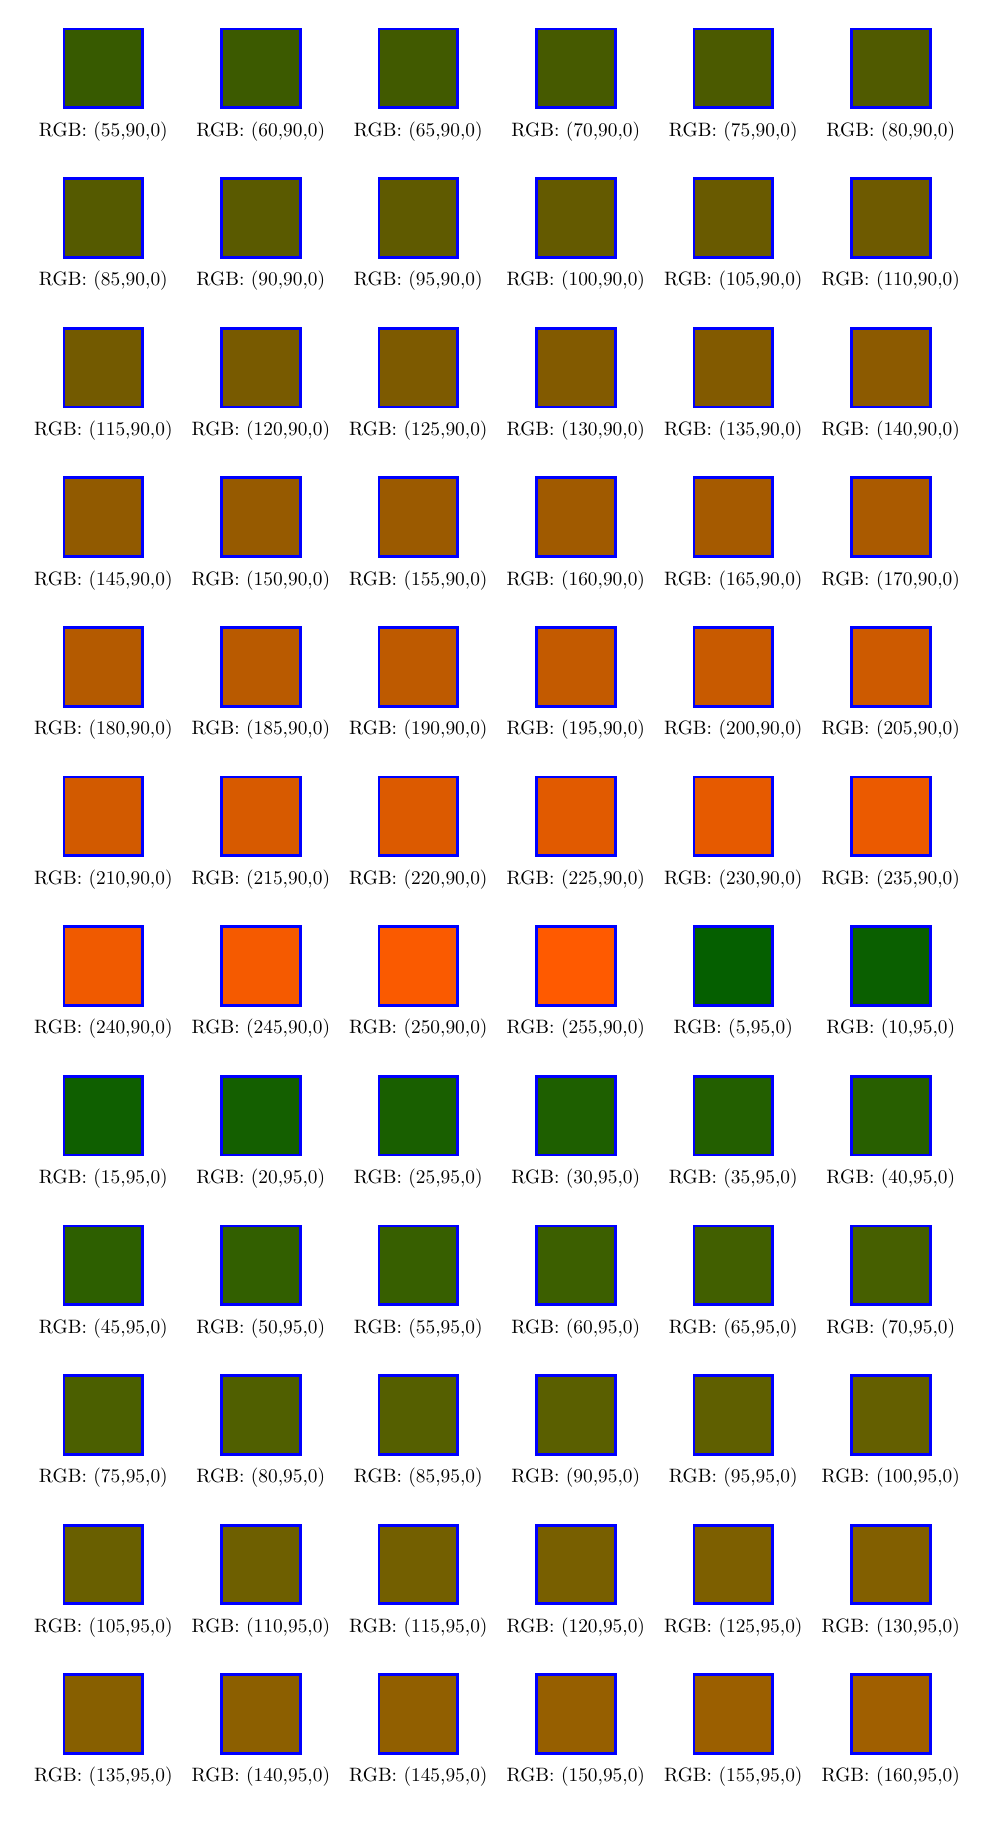
\begin{tikzpicture}

    \filldraw[draw=blue,line width=1,fill=colorR55G90B0]
    (0,0) rectangle (1,1);

    \node[scale=0.7] at (0.5,-0.3) {RGB: (55,90,0)};



    \begin{scope}[xshift=2cm]

      \filldraw[draw=blue,line width=1,fill=colorR60G90B0]
      (0,0) rectangle (1,1);

      \node[scale=0.7] at (0.5,-0.3) {RGB: (60,90,0)};

    \end{scope}



    \begin{scope}[xshift=4cm]

      \filldraw[draw=blue,line width=1,fill=colorR65G90B0]
      (0,0) rectangle (1,1);

      \node[scale=0.7] at (0.5,-0.3) {RGB: (65,90,0)};

    \end{scope}



    \begin{scope}[xshift=6cm]

      \filldraw[draw=blue,line width=1,fill=colorR70G90B0]
      (0,0) rectangle (1,1);

      \node[scale=0.7] at (0.5,-0.3) {RGB: (70,90,0)};

    \end{scope}



    \begin{scope}[xshift=8cm]

      \filldraw[draw=blue,line width=1,fill=colorR75G90B0]
      (0,0) rectangle (1,1);

      \node[scale=0.7] at (0.5,-0.3) {RGB: (75,90,0)};

    \end{scope}



    \begin{scope}[xshift=10cm]

      \filldraw[draw=blue,line width=1,fill=colorR80G90B0]
      (0,0) rectangle (1,1);

      \node[scale=0.7] at (0.5,-0.3) {RGB: (80,90,0)};

    \end{scope}







    \begin{scope}[yshift=-1.9cm]

      \filldraw[draw=blue,line width=1,fill=colorR85G90B0]
      (0,0) rectangle (1,1);

      \node[scale=0.7] at (0.5,-0.3) {RGB: (85,90,0)};

    \end{scope}



    \begin{scope}[xshift=2cm,yshift=-1.9cm]

      \filldraw[draw=blue,line width=1,fill=colorR90G90B0]
      (0,0) rectangle (1,1);

      \node[scale=0.7] at (0.5,-0.3) {RGB: (90,90,0)};

    \end{scope}



    \begin{scope}[xshift=4cm,yshift=-1.9cm]

      \filldraw[draw=blue,line width=1,fill=colorR95G90B0]
      (0,0) rectangle (1,1);

      \node[scale=0.7] at (0.5,-0.3) {RGB: (95,90,0)};

    \end{scope}



    \begin{scope}[xshift=6cm,yshift=-1.9cm]

      \filldraw[draw=blue,line width=1,fill=colorR100G90B0]
      (0,0) rectangle (1,1);

      \node[scale=0.7] at (0.5,-0.3) {RGB: (100,90,0)};

    \end{scope}



    \begin{scope}[xshift=8cm,yshift=-1.9cm]

      \filldraw[draw=blue,line width=1,fill=colorR105G90B0]
      (0,0) rectangle (1,1);

      \node[scale=0.7] at (0.5,-0.3) {RGB: (105,90,0)};

    \end{scope}



    \begin{scope}[xshift=10cm,yshift=-1.9cm]

      \filldraw[draw=blue,line width=1,fill=colorR110G90B0]
      (0,0) rectangle (1,1);

      \node[scale=0.7] at (0.5,-0.3) {RGB: (110,90,0)};

    \end{scope}







    \begin{scope}[yshift=-3.8cm]

      \filldraw[draw=blue,line width=1,fill=colorR115G90B0]
      (0,0) rectangle (1,1);

      \node[scale=0.7] at (0.5,-0.3) {RGB: (115,90,0)};

    \end{scope}



    \begin{scope}[xshift=2cm,yshift=-3.8cm]

      \filldraw[draw=blue,line width=1,fill=colorR120G90B0]
      (0,0) rectangle (1,1);

      \node[scale=0.7] at (0.5,-0.3) {RGB: (120,90,0)};

    \end{scope}



    \begin{scope}[xshift=4cm,yshift=-3.8cm]

      \filldraw[draw=blue,line width=1,fill=colorR125G90B0]
      (0,0) rectangle (1,1);

      \node[scale=0.7] at (0.5,-0.3) {RGB: (125,90,0)};

    \end{scope}



    \begin{scope}[xshift=6cm,yshift=-3.8cm]

      \filldraw[draw=blue,line width=1,fill=colorR130G90B0]
      (0,0) rectangle (1,1);

      \node[scale=0.7] at (0.5,-0.3) {RGB: (130,90,0)};

    \end{scope}



    \begin{scope}[xshift=8cm,yshift=-3.8cm]

      \filldraw[draw=blue,line width=1,fill=colorR130G90B0]
      (0,0) rectangle (1,1);

      \node[scale=0.7] at (0.5,-0.3) {RGB: (135,90,0)};

    \end{scope}



    \begin{scope}[xshift=10cm,yshift=-3.8cm]

      \filldraw[draw=blue,line width=1,fill=colorR140G90B0]
      (0,0) rectangle (1,1);

      \node[scale=0.7] at (0.5,-0.3) {RGB: (140,90,0)};

    \end{scope}







    \begin{scope}[yshift=-5.7cm]

      \filldraw[draw=blue,line width=1,fill=colorR145G90B0]
      (0,0) rectangle (1,1);

      \node[scale=0.7] at (0.5,-0.3) {RGB: (145,90,0)};

    \end{scope}



    \begin{scope}[xshift=2cm,yshift=-5.7cm]

      \filldraw[draw=blue,line width=1,fill=colorR150G90B0]
      (0,0) rectangle (1,1);

      \node[scale=0.7] at (0.5,-0.3) {RGB: (150,90,0)};

    \end{scope}



    \begin{scope}[xshift=4cm,yshift=-5.7cm]

      \filldraw[draw=blue,line width=1,fill=colorR155G90B0]
      (0,0) rectangle (1,1);

      \node[scale=0.7] at (0.5,-0.3) {RGB: (155,90,0)};

    \end{scope}



    \begin{scope}[xshift=6cm,yshift=-5.7cm]

      \filldraw[draw=blue,line width=1,fill=colorR160G90B0]
      (0,0) rectangle (1,1);

      \node[scale=0.7] at (0.5,-0.3) {RGB: (160,90,0)};

    \end{scope}



    \begin{scope}[xshift=8cm,yshift=-5.7cm]

      \filldraw[draw=blue,line width=1,fill=colorR165G90B0]
      (0,0) rectangle (1,1);

      \node[scale=0.7] at (0.5,-0.3) {RGB: (165,90,0)};

    \end{scope}



    \begin{scope}[xshift=10cm,yshift=-5.7cm]

      \filldraw[draw=blue,line width=1,fill=colorR170G90B0]
      (0,0) rectangle (1,1);

      \node[scale=0.7] at (0.5,-0.3) {RGB: (170,90,0)};

    \end{scope}







    \begin{scope}[yshift=-7.6cm]

      \filldraw[draw=blue,line width=1,fill=colorR180G90B0]
      (0,0) rectangle (1,1);

      \node[scale=0.7] at (0.5,-0.3) {RGB: (180,90,0)};

    \end{scope}



    \begin{scope}[xshift=2cm,yshift=-7.6cm]

      \filldraw[draw=blue,line width=1,fill=colorR185G90B0]
      (0,0) rectangle (1,1);

      \node[scale=0.7] at (0.5,-0.3) {RGB: (185,90,0)};

    \end{scope}



    \begin{scope}[xshift=4cm,yshift=-7.6cm]

      \filldraw[draw=blue,line width=1,fill=colorR190G90B0]
      (0,0) rectangle (1,1);

      \node[scale=0.7] at (0.5,-0.3) {RGB: (190,90,0)};

    \end{scope}



    \begin{scope}[xshift=6cm,yshift=-7.6cm]

      \filldraw[draw=blue,line width=1,fill=colorR195G90B0]
      (0,0) rectangle (1,1);

      \node[scale=0.7] at (0.5,-0.3) {RGB: (195,90,0)};

    \end{scope}



    \begin{scope}[xshift=8cm,yshift=-7.6cm]

      \filldraw[draw=blue,line width=1,fill=colorR200G90B0]
      (0,0) rectangle (1,1);

      \node[scale=0.7] at (0.5,-0.3) {RGB: (200,90,0)};

    \end{scope}



    \begin{scope}[xshift=10cm,yshift=-7.6cm]

      \filldraw[draw=blue,line width=1,fill=colorR205G90B0]
      (0,0) rectangle (1,1);

      \node[scale=0.7] at (0.5,-0.3) {RGB: (205,90,0)};

    \end{scope}







    \begin{scope}[yshift=-9.5cm]

      \filldraw[draw=blue,line width=1,fill=colorR210G90B0]
      (0,0) rectangle (1,1);

      \node[scale=0.7] at (0.5,-0.3) {RGB: (210,90,0)};

    \end{scope}



    \begin{scope}[xshift=2cm,yshift=-9.5cm]

      \filldraw[draw=blue,line width=1,fill=colorR215G90B0]
      (0,0) rectangle (1,1);

      \node[scale=0.7] at (0.5,-0.3) {RGB: (215,90,0)};

    \end{scope}



    \begin{scope}[xshift=4cm,yshift=-9.5cm]

      \filldraw[draw=blue,line width=1,fill=colorR220G90B0]
      (0,0) rectangle (1,1);

      \node[scale=0.7] at (0.5,-0.3) {RGB: (220,90,0)};

    \end{scope}



    \begin{scope}[xshift=6cm,yshift=-9.5cm]

      \filldraw[draw=blue,line width=1,fill=colorR225G90B0]
      (0,0) rectangle (1,1);

      \node[scale=0.7] at (0.5,-0.3) {RGB: (225,90,0)};

    \end{scope}



    \begin{scope}[xshift=8cm,yshift=-9.5cm]

      \filldraw[draw=blue,line width=1,fill=colorR230G90B0]
      (0,0) rectangle (1,1);

      \node[scale=0.7] at (0.5,-0.3) {RGB: (230,90,0)};

    \end{scope}



    \begin{scope}[xshift=10cm,yshift=-9.5cm]

      \filldraw[draw=blue,line width=1,fill=colorR235G90B0]
      (0,0) rectangle (1,1);

      \node[scale=0.7] at (0.5,-0.3) {RGB: (235,90,0)};

    \end{scope}







    \begin{scope}[yshift=-11.4cm]

      \filldraw[draw=blue,line width=1,fill=colorR240G90B0]
      (0,0) rectangle (1,1);

      \node[scale=0.7] at (0.5,-0.3) {RGB: (240,90,0)};

    \end{scope}



    \begin{scope}[xshift=2cm,yshift=-11.4cm]

      \filldraw[draw=blue,line width=1,fill=colorR245G90B0]
      (0,0) rectangle (1,1);

      \node[scale=0.7] at (0.5,-0.3) {RGB: (245,90,0)};

    \end{scope}



    \begin{scope}[xshift=4cm,yshift=-11.4cm]

      \filldraw[draw=blue,line width=1,fill=colorR250G90B0]
      (0,0) rectangle (1,1);

      \node[scale=0.7] at (0.5,-0.3) {RGB: (250,90,0)};

    \end{scope}



    \begin{scope}[xshift=6cm,yshift=-11.4cm]

      \filldraw[draw=blue,line width=1,fill=colorR255G90B0]
      (0,0) rectangle (1,1);

      \node[scale=0.7] at (0.5,-0.3) {RGB: (255,90,0)};

    \end{scope}



    \begin{scope}[xshift=8cm,yshift=-11.4cm]

      \filldraw[draw=blue,line width=1,fill=colorR5G95B0]
      (0,0) rectangle (1,1);

      \node[scale=0.7] at (0.5,-0.3) {RGB: (5,95,0)};

    \end{scope}



    \begin{scope}[xshift=10cm,yshift=-11.4cm]

      \filldraw[draw=blue,line width=1,fill=colorR10G95B0]
      (0,0) rectangle (1,1);

      \node[scale=0.7] at (0.5,-0.3) {RGB: (10,95,0)};

    \end{scope}







    \begin{scope}[yshift=-13.3cm]

      \filldraw[draw=blue,line width=1,fill=colorR15G95B0]
      (0,0) rectangle (1,1);

      \node[scale=0.7] at (0.5,-0.3) {RGB: (15,95,0)};

    \end{scope}



    \begin{scope}[xshift=2cm,yshift=-13.3cm]

      \filldraw[draw=blue,line width=1,fill=colorR20G95B0]
      (0,0) rectangle (1,1);

      \node[scale=0.7] at (0.5,-0.3) {RGB: (20,95,0)};

    \end{scope}



    \begin{scope}[xshift=4cm,yshift=-13.3cm]

      \filldraw[draw=blue,line width=1,fill=colorR25G95B0]
      (0,0) rectangle (1,1);

      \node[scale=0.7] at (0.5,-0.3) {RGB: (25,95,0)};

    \end{scope}



    \begin{scope}[xshift=6cm,yshift=-13.3cm]

      \filldraw[draw=blue,line width=1,fill=colorR30G95B0]
      (0,0) rectangle (1,1);

      \node[scale=0.7] at (0.5,-0.3) {RGB: (30,95,0)};

    \end{scope}



    \begin{scope}[xshift=8cm,yshift=-13.3cm]

      \filldraw[draw=blue,line width=1,fill=colorR35G95B0]
      (0,0) rectangle (1,1);

      \node[scale=0.7] at (0.5,-0.3) {RGB: (35,95,0)};

    \end{scope}



    \begin{scope}[xshift=10cm,yshift=-13.3cm]

      \filldraw[draw=blue,line width=1,fill=colorR40G95B0]
      (0,0) rectangle (1,1);

      \node[scale=0.7] at (0.5,-0.3) {RGB: (40,95,0)};

    \end{scope}







    \begin{scope}[yshift=-15.2cm]

      \filldraw[draw=blue,line width=1,fill=colorR45G95B0]
      (0,0) rectangle (1,1);

      \node[scale=0.7] at (0.5,-0.3) {RGB: (45,95,0)};

    \end{scope}



    \begin{scope}[xshift=2cm,yshift=-15.2cm]

      \filldraw[draw=blue,line width=1,fill=colorR50G95B0]
      (0,0) rectangle (1,1);

      \node[scale=0.7] at (0.5,-0.3) {RGB: (50,95,0)};

    \end{scope}



    \begin{scope}[xshift=4cm,yshift=-15.2cm]

      \filldraw[draw=blue,line width=1,fill=colorR55G95B0]
      (0,0) rectangle (1,1);

      \node[scale=0.7] at (0.5,-0.3) {RGB: (55,95,0)};

    \end{scope}



    \begin{scope}[xshift=6cm,yshift=-15.2cm]

      \filldraw[draw=blue,line width=1,fill=colorR60G95B0]
      (0,0) rectangle (1,1);

      \node[scale=0.7] at (0.5,-0.3) {RGB: (60,95,0)};

    \end{scope}



    \begin{scope}[xshift=8cm,yshift=-15.2cm]

      \filldraw[draw=blue,line width=1,fill=colorR65G95B0]
      (0,0) rectangle (1,1);

      \node[scale=0.7] at (0.5,-0.3) {RGB: (65,95,0)};

    \end{scope}



    \begin{scope}[xshift=10cm,yshift=-15.2cm]

      \filldraw[draw=blue,line width=1,fill=colorR70G95B0]
      (0,0) rectangle (1,1);

      \node[scale=0.7] at (0.5,-0.3) {RGB: (70,95,0)};

    \end{scope}







    \begin{scope}[yshift=-17.1cm]

      \filldraw[draw=blue,line width=1,fill=colorR75G95B0]
      (0,0) rectangle (1,1);

      \node[scale=0.7] at (0.5,-0.3) {RGB: (75,95,0)};

    \end{scope}



    \begin{scope}[xshift=2cm,yshift=-17.1cm]

      \filldraw[draw=blue,line width=1,fill=colorR80G95B0]
      (0,0) rectangle (1,1);

      \node[scale=0.7] at (0.5,-0.3) {RGB: (80,95,0)};

    \end{scope}



    \begin{scope}[xshift=4cm,yshift=-17.1cm]

      \filldraw[draw=blue,line width=1,fill=colorR85G95B0]
      (0,0) rectangle (1,1);

      \node[scale=0.7] at (0.5,-0.3) {RGB: (85,95,0)};

    \end{scope}



    \begin{scope}[xshift=6cm,yshift=-17.1cm]

      \filldraw[draw=blue,line width=1,fill=colorR90G95B0]
      (0,0) rectangle (1,1);

      \node[scale=0.7] at (0.5,-0.3) {RGB: (90,95,0)};

    \end{scope}



    \begin{scope}[xshift=8cm,yshift=-17.1cm]

      \filldraw[draw=blue,line width=1,fill=colorR95G95B0]
      (0,0) rectangle (1,1);

      \node[scale=0.7] at (0.5,-0.3) {RGB: (95,95,0)};

    \end{scope}



    \begin{scope}[xshift=10cm,yshift=-17.1cm]

      \filldraw[draw=blue,line width=1,fill=colorR100G95B0]
      (0,0) rectangle (1,1);

      \node[scale=0.7] at (0.5,-0.3) {RGB: (100,95,0)};

    \end{scope}







    \begin{scope}[yshift=-19cm]

      \filldraw[draw=blue,line width=1,fill=colorR105G95B0]
      (0,0) rectangle (1,1);

      \node[scale=0.7] at (0.5,-0.3) {RGB: (105,95,0)};

    \end{scope}



    \begin{scope}[xshift=2cm,yshift=-19cm]

      \filldraw[draw=blue,line width=1,fill=colorR110G95B0]
      (0,0) rectangle (1,1);

      \node[scale=0.7] at (0.5,-0.3) {RGB: (110,95,0)};

    \end{scope}



    \begin{scope}[xshift=4cm,yshift=-19cm]

      \filldraw[draw=blue,line width=1,fill=colorR115G95B0]
      (0,0) rectangle (1,1);

      \node[scale=0.7] at (0.5,-0.3) {RGB: (115,95,0)};

    \end{scope}



    \begin{scope}[xshift=6cm,yshift=-19cm]

      \filldraw[draw=blue,line width=1,fill=colorR120G95B0]
      (0,0) rectangle (1,1);

      \node[scale=0.7] at (0.5,-0.3) {RGB: (120,95,0)};

    \end{scope}



    \begin{scope}[xshift=8cm,yshift=-19cm]

      \filldraw[draw=blue,line width=1,fill=colorR125G95B0]
      (0,0) rectangle (1,1);

      \node[scale=0.7] at (0.5,-0.3) {RGB: (125,95,0)};

    \end{scope}



    \begin{scope}[xshift=10cm,yshift=-19cm]

      \filldraw[draw=blue,line width=1,fill=colorR130G95B0]
      (0,0) rectangle (1,1);

      \node[scale=0.7] at (0.5,-0.3) {RGB: (130,95,0)};

    \end{scope}







    \begin{scope}[yshift=-20.9cm]

      \filldraw[draw=blue,line width=1,fill=colorR135G95B0]
      (0,0) rectangle (1,1);

      \node[scale=0.7] at (0.5,-0.3) {RGB: (135,95,0)};

    \end{scope}



    \begin{scope}[xshift=2cm,yshift=-20.9cm]

      \filldraw[draw=blue,line width=1,fill=colorR140G95B0]
      (0,0) rectangle (1,1);

      \node[scale=0.7] at (0.5,-0.3) {RGB: (140,95,0)};

    \end{scope}



    \begin{scope}[xshift=4cm,yshift=-20.9cm]

      \filldraw[draw=blue,line width=1,fill=colorR145G95B0]
      (0,0) rectangle (1,1);

      \node[scale=0.7] at (0.5,-0.3) {RGB: (145,95,0)};

    \end{scope}



    \begin{scope}[xshift=6cm,yshift=-20.9cm]

      \filldraw[draw=blue,line width=1,fill=colorR150G95B0]
      (0,0) rectangle (1,1);

      \node[scale=0.7] at (0.5,-0.3) {RGB: (150,95,0)};

    \end{scope}



    \begin{scope}[xshift=8cm,yshift=-20.9cm]

      \filldraw[draw=blue,line width=1,fill=colorR155G95B0]
      (0,0) rectangle (1,1);

      \node[scale=0.7] at (0.5,-0.3) {RGB: (155,95,0)};

    \end{scope}



    \begin{scope}[xshift=10cm,yshift=-20.9cm]

      \filldraw[draw=blue,line width=1,fill=colorR160G95B0]
      (0,0) rectangle (1,1);

      \node[scale=0.7] at (0.5,-0.3) {RGB: (160,95,0)};

    \end{scope}

  \end{tikzpicture}

  \caption{Mixed colors in~RGB system: $(55,90,0)$--$(255,90,0)$,
    $(5,95,0)$--$(160,95,0)$}



  \label{fig:Mixed-colors-Part-04}

\end{figure}
% ##################





% ##################
\begin{figure}

  \centering


  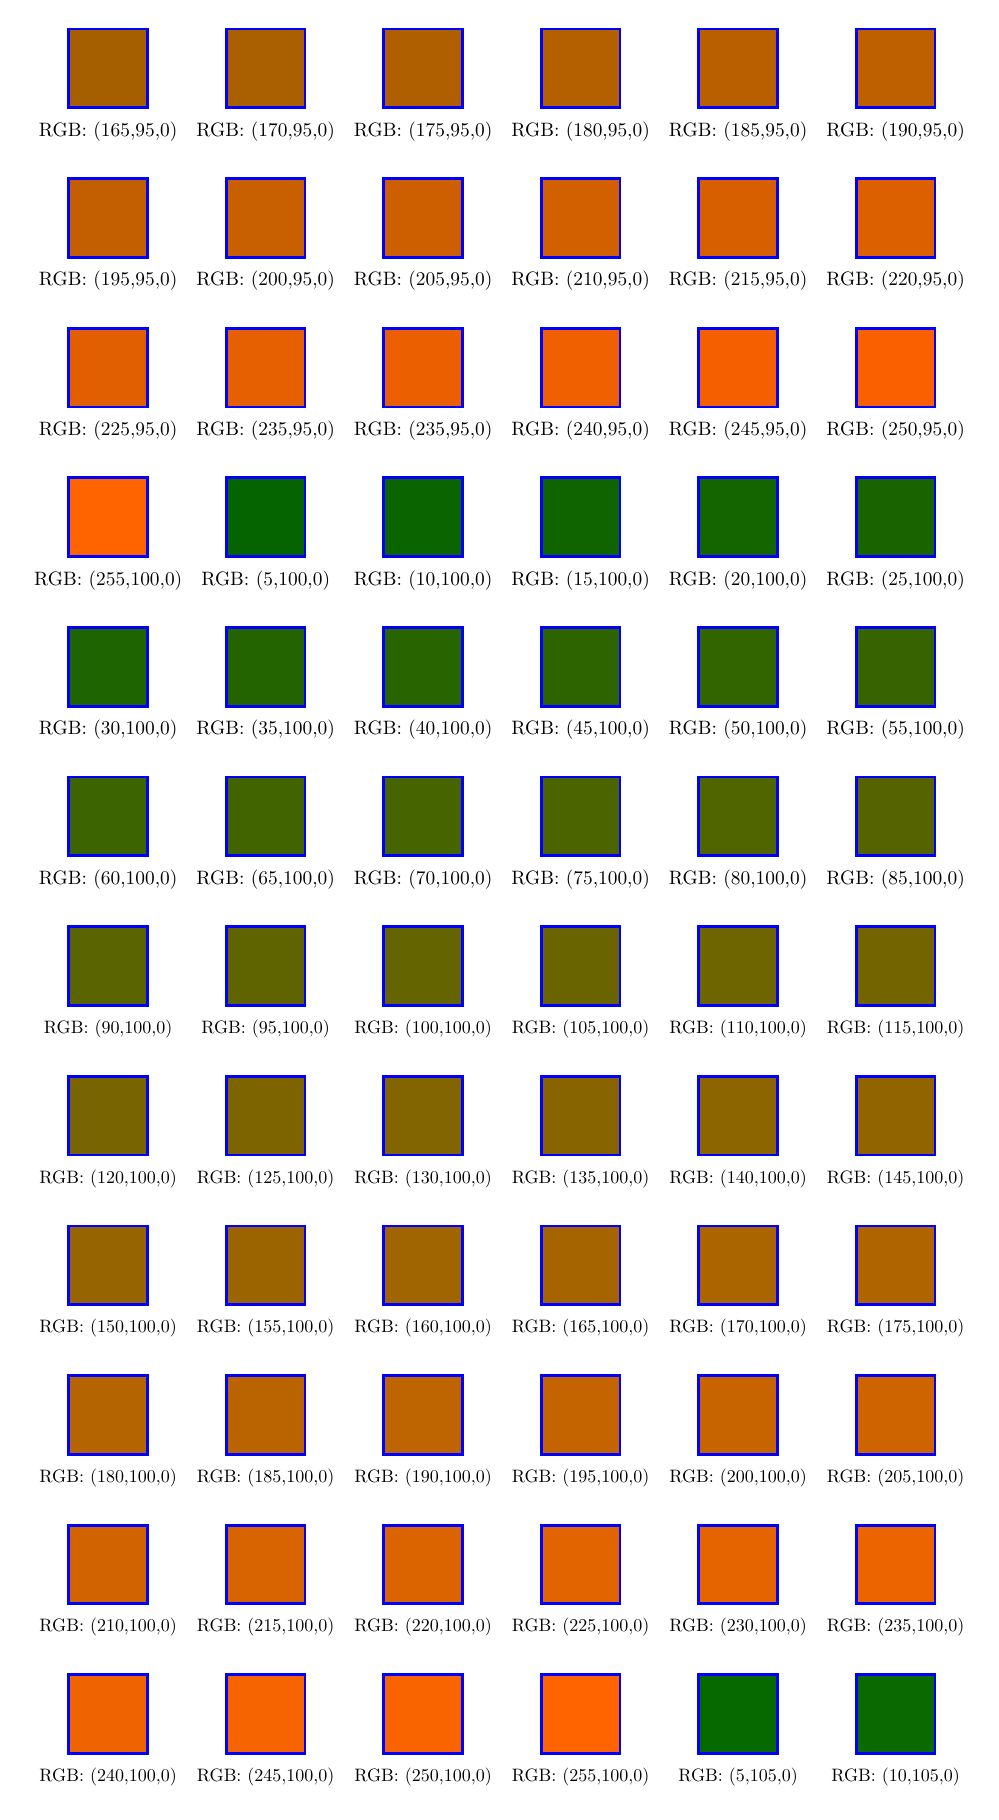
\begin{tikzpicture}

    \filldraw[draw=blue,line width=1,fill=colorR165G95B0]
    (0,0) rectangle (1,1);

    \node[scale=0.7] at (0.5,-0.3) {RGB: (165,95,0)};



    \begin{scope}[xshift=2cm]

      \filldraw[draw=blue,line width=1,fill=colorR170G95B0]
      (0,0) rectangle (1,1);

      \node[scale=0.7] at (0.5,-0.3) {RGB: (170,95,0)};

    \end{scope}



    \begin{scope}[xshift=4cm]

      \filldraw[draw=blue,line width=1,fill=colorR175G95B0]
      (0,0) rectangle (1,1);

      \node[scale=0.7] at (0.5,-0.3) {RGB: (175,95,0)};

    \end{scope}



    \begin{scope}[xshift=6cm]

      \filldraw[draw=blue,line width=1,fill=colorR180G95B0]
      (0,0) rectangle (1,1);

      \node[scale=0.7] at (0.5,-0.3) {RGB: (180,95,0)};

    \end{scope}



    \begin{scope}[xshift=8cm]

      \filldraw[draw=blue,line width=1,fill=colorR185G95B0]
      (0,0) rectangle (1,1);

      \node[scale=0.7] at (0.5,-0.3) {RGB: (185,95,0)};

    \end{scope}



    \begin{scope}[xshift=10cm]

      \filldraw[draw=blue,line width=1,fill=colorR190G95B0]
      (0,0) rectangle (1,1);

      \node[scale=0.7] at (0.5,-0.3) {RGB: (190,95,0)};

    \end{scope}







    \begin{scope}[yshift=-1.9cm]

      \filldraw[draw=blue,line width=1,fill=colorR195G95B0]
      (0,0) rectangle (1,1);

      \node[scale=0.7] at (0.5,-0.3) {RGB: (195,95,0)};

    \end{scope}



    \begin{scope}[xshift=2cm,yshift=-1.9cm]

      \filldraw[draw=blue,line width=1,fill=colorR200G95B0]
      (0,0) rectangle (1,1);

      \node[scale=0.7] at (0.5,-0.3) {RGB: (200,95,0)};

    \end{scope}



    \begin{scope}[xshift=4cm,yshift=-1.9cm]

      \filldraw[draw=blue,line width=1,fill=colorR205G95B0]
      (0,0) rectangle (1,1);

      \node[scale=0.7] at (0.5,-0.3) {RGB: (205,95,0)};

    \end{scope}



    \begin{scope}[xshift=6cm,yshift=-1.9cm]

      \filldraw[draw=blue,line width=1,fill=colorR210G95B0]
      (0,0) rectangle (1,1);

      \node[scale=0.7] at (0.5,-0.3) {RGB: (210,95,0)};

    \end{scope}



    \begin{scope}[xshift=8cm,yshift=-1.9cm]

      \filldraw[draw=blue,line width=1,fill=colorR215G95B0]
      (0,0) rectangle (1,1);

      \node[scale=0.7] at (0.5,-0.3) {RGB: (215,95,0)};

    \end{scope}



    \begin{scope}[xshift=10cm,yshift=-1.9cm]

      \filldraw[draw=blue,line width=1,fill=colorR220G95B0]
      (0,0) rectangle (1,1);

      \node[scale=0.7] at (0.5,-0.3) {RGB: (220,95,0)};

    \end{scope}







    \begin{scope}[yshift=-3.8cm]

      \filldraw[draw=blue,line width=1,fill=colorR225G95B0]
      (0,0) rectangle (1,1);

      \node[scale=0.7] at (0.5,-0.3) {RGB: (225,95,0)};

    \end{scope}



    \begin{scope}[xshift=2cm,yshift=-3.8cm]

      \filldraw[draw=blue,line width=1,fill=colorR230G95B0]
      (0,0) rectangle (1,1);

      \node[scale=0.7] at (0.5,-0.3) {RGB: (235,95,0)};

    \end{scope}



    \begin{scope}[xshift=4cm,yshift=-3.8cm]

      \filldraw[draw=blue,line width=1,fill=colorR235G95B0]
      (0,0) rectangle (1,1);

      \node[scale=0.7] at (0.5,-0.3) {RGB: (235,95,0)};

    \end{scope}



    \begin{scope}[xshift=6cm,yshift=-3.8cm]

      \filldraw[draw=blue,line width=1,fill=colorR240G95B0]
      (0,0) rectangle (1,1);

      \node[scale=0.7] at (0.5,-0.3) {RGB: (240,95,0)};

    \end{scope}



    \begin{scope}[xshift=8cm,yshift=-3.8cm]

      \filldraw[draw=blue,line width=1,fill=colorR245G95B0]
      (0,0) rectangle (1,1);

      \node[scale=0.7] at (0.5,-0.3) {RGB: (245,95,0)};

    \end{scope}



    \begin{scope}[xshift=10cm,yshift=-3.8cm]

      \filldraw[draw=blue,line width=1,fill=colorR250G95B0]
      (0,0) rectangle (1,1);

      \node[scale=0.7] at (0.5,-0.3) {RGB: (250,95,0)};

    \end{scope}







    \begin{scope}[yshift=-5.7cm]

      \filldraw[draw=blue,line width=1,fill=colorR255G100B0]
      (0,0) rectangle (1,1);

      \node[scale=0.7] at (0.5,-0.3) {RGB: (255,100,0)};

    \end{scope}



    \begin{scope}[xshift=2cm,yshift=-5.7cm]

      \filldraw[draw=blue,line width=1,fill=colorR5G100B0]
      (0,0) rectangle (1,1);

      \node[scale=0.7] at (0.5,-0.3) {RGB: (5,100,0)};

    \end{scope}



    \begin{scope}[xshift=4cm,yshift=-5.7cm]

      \filldraw[draw=blue,line width=1,fill=colorR10G100B0]
      (0,0) rectangle (1,1);

      \node[scale=0.7] at (0.5,-0.3) {RGB: (10,100,0)};

    \end{scope}



    \begin{scope}[xshift=6cm,yshift=-5.7cm]

      \filldraw[draw=blue,line width=1,fill=colorR15G100B0]
      (0,0) rectangle (1,1);

      \node[scale=0.7] at (0.5,-0.3) {RGB: (15,100,0)};

    \end{scope}



    \begin{scope}[xshift=8cm,yshift=-5.7cm]

      \filldraw[draw=blue,line width=1,fill=colorR20G100B0]
      (0,0) rectangle (1,1);

      \node[scale=0.7] at (0.5,-0.3) {RGB: (20,100,0)};

    \end{scope}



    \begin{scope}[xshift=10cm,yshift=-5.7cm]

      \filldraw[draw=blue,line width=1,fill=colorR25G100B0]
      (0,0) rectangle (1,1);

      \node[scale=0.7] at (0.5,-0.3) {RGB: (25,100,0)};

    \end{scope}







    \begin{scope}[yshift=-7.6cm]

      \filldraw[draw=blue,line width=1,fill=colorR30G100B0]
      (0,0) rectangle (1,1);

      \node[scale=0.7] at (0.5,-0.3) {RGB: (30,100,0)};

    \end{scope}



    \begin{scope}[xshift=2cm,yshift=-7.6cm]

      \filldraw[draw=blue,line width=1,fill=colorR35G100B0]
      (0,0) rectangle (1,1);

      \node[scale=0.7] at (0.5,-0.3) {RGB: (35,100,0)};

    \end{scope}



    \begin{scope}[xshift=4cm,yshift=-7.6cm]

      \filldraw[draw=blue,line width=1,fill=colorR40G100B0]
      (0,0) rectangle (1,1);

      \node[scale=0.7] at (0.5,-0.3) {RGB: (40,100,0)};

    \end{scope}



    \begin{scope}[xshift=6cm,yshift=-7.6cm]

      \filldraw[draw=blue,line width=1,fill=colorR45G100B0]
      (0,0) rectangle (1,1);

      \node[scale=0.7] at (0.5,-0.3) {RGB: (45,100,0)};

    \end{scope}



    \begin{scope}[xshift=8cm,yshift=-7.6cm]

      \filldraw[draw=blue,line width=1,fill=colorR50G100B0]
      (0,0) rectangle (1,1);

      \node[scale=0.7] at (0.5,-0.3) {RGB: (50,100,0)};

    \end{scope}



    \begin{scope}[xshift=10cm,yshift=-7.6cm]

      \filldraw[draw=blue,line width=1,fill=colorR55G100B0]
      (0,0) rectangle (1,1);

      \node[scale=0.7] at (0.5,-0.3) {RGB: (55,100,0)};

    \end{scope}







    \begin{scope}[yshift=-9.5cm]

      \filldraw[draw=blue,line width=1,fill=colorR60G100B0]
      (0,0) rectangle (1,1);

      \node[scale=0.7] at (0.5,-0.3) {RGB: (60,100,0)};

    \end{scope}



    \begin{scope}[xshift=2cm,yshift=-9.5cm]

      \filldraw[draw=blue,line width=1,fill=colorR65G100B0]
      (0,0) rectangle (1,1);

      \node[scale=0.7] at (0.5,-0.3) {RGB: (65,100,0)};

    \end{scope}



    \begin{scope}[xshift=4cm,yshift=-9.5cm]

      \filldraw[draw=blue,line width=1,fill=colorR70G100B0]
      (0,0) rectangle (1,1);

      \node[scale=0.7] at (0.5,-0.3) {RGB: (70,100,0)};

    \end{scope}



    \begin{scope}[xshift=6cm,yshift=-9.5cm]

      \filldraw[draw=blue,line width=1,fill=colorR75G100B0]
      (0,0) rectangle (1,1);

      \node[scale=0.7] at (0.5,-0.3) {RGB: (75,100,0)};

    \end{scope}



    \begin{scope}[xshift=8cm,yshift=-9.5cm]

      \filldraw[draw=blue,line width=1,fill=colorR80G100B0]
      (0,0) rectangle (1,1);

      \node[scale=0.7] at (0.5,-0.3) {RGB: (80,100,0)};

    \end{scope}



    \begin{scope}[xshift=10cm,yshift=-9.5cm]

      \filldraw[draw=blue,line width=1,fill=colorR85G100B0]
      (0,0) rectangle (1,1);

      \node[scale=0.7] at (0.5,-0.3) {RGB: (85,100,0)};

    \end{scope}







    \begin{scope}[yshift=-11.4cm]

      \filldraw[draw=blue,line width=1,fill=colorR90G100B0]
      (0,0) rectangle (1,1);

      \node[scale=0.65] at (0.5,-0.3) {RGB: (90,100,0)};

    \end{scope}



    \begin{scope}[xshift=2cm,yshift=-11.4cm]

      \filldraw[draw=blue,line width=1,fill=colorR95G100B0]
      (0,0) rectangle (1,1);

      \node[scale=0.65] at (0.5,-0.3) {RGB: (95,100,0)};

    \end{scope}



    \begin{scope}[xshift=4cm,yshift=-11.4cm]

      \filldraw[draw=blue,line width=1,fill=colorR100G100B0]
      (0,0) rectangle (1,1);

      \node[scale=0.65] at (0.5,-0.3) {RGB: (100,100,0)};

    \end{scope}



    \begin{scope}[xshift=6cm,yshift=-11.4cm]

      \filldraw[draw=blue,line width=1,fill=colorR105G100B0]
      (0,0) rectangle (1,1);

      \node[scale=0.65] at (0.5,-0.3) {RGB: (105,100,0)};

    \end{scope}



    \begin{scope}[xshift=8cm,yshift=-11.4cm]

      \filldraw[draw=blue,line width=1,fill=colorR110G100B0]
      (0,0) rectangle (1,1);

      \node[scale=0.65] at (0.5,-0.3) {RGB: (110,100,0)};

    \end{scope}



    \begin{scope}[xshift=10cm,yshift=-11.4cm]

      \filldraw[draw=blue,line width=1,fill=colorR115G100B0]
      (0,0) rectangle (1,1);

      \node[scale=0.65] at (0.5,-0.3) {RGB: (115,100,0)};

    \end{scope}







    \begin{scope}[yshift=-13.3cm]

      \filldraw[draw=blue,line width=1,fill=colorR120G100B0]
      (0,0) rectangle (1,1);

      \node[scale=0.65] at (0.5,-0.3) {RGB: (120,100,0)};

    \end{scope}



    \begin{scope}[xshift=2cm,yshift=-13.3cm]

      \filldraw[draw=blue,line width=1,fill=colorR125G100B0]
      (0,0) rectangle (1,1);

      \node[scale=0.65] at (0.5,-0.3) {RGB: (125,100,0)};

    \end{scope}



    \begin{scope}[xshift=4cm,yshift=-13.3cm]

      \filldraw[draw=blue,line width=1,fill=colorR130G100B0]
      (0,0) rectangle (1,1);

      \node[scale=0.65] at (0.5,-0.3) {RGB: (130,100,0)};

    \end{scope}



    \begin{scope}[xshift=6cm,yshift=-13.3cm]

      \filldraw[draw=blue,line width=1,fill=colorR135G100B0]
      (0,0) rectangle (1,1);

      \node[scale=0.65] at (0.5,-0.3) {RGB: (135,100,0)};

    \end{scope}



    \begin{scope}[xshift=8cm,yshift=-13.3cm]

      \filldraw[draw=blue,line width=1,fill=colorR140G100B0]
      (0,0) rectangle (1,1);

      \node[scale=0.65] at (0.5,-0.3) {RGB: (140,100,0)};

    \end{scope}



    \begin{scope}[xshift=10cm,yshift=-13.3cm]

      \filldraw[draw=blue,line width=1,fill=colorR145G100B0]
      (0,0) rectangle (1,1);

      \node[scale=0.65] at (0.5,-0.3) {RGB: (145,100,0)};

    \end{scope}







    \begin{scope}[yshift=-15.2cm]

      \filldraw[draw=blue,line width=1,fill=colorR150G100B0]
      (0,0) rectangle (1,1);

      \node[scale=0.65] at (0.5,-0.3) {RGB: (150,100,0)};

    \end{scope}



    \begin{scope}[xshift=2cm,yshift=-15.2cm]

      \filldraw[draw=blue,line width=1,fill=colorR155G100B0]
      (0,0) rectangle (1,1);

      \node[scale=0.65] at (0.5,-0.3) {RGB: (155,100,0)};

    \end{scope}



    \begin{scope}[xshift=4cm,yshift=-15.2cm]

      \filldraw[draw=blue,line width=1,fill=colorR160G100B0]
      (0,0) rectangle (1,1);

      \node[scale=0.65] at (0.5,-0.3) {RGB: (160,100,0)};

    \end{scope}



    \begin{scope}[xshift=6cm,yshift=-15.2cm]

      \filldraw[draw=blue,line width=1,fill=colorR165G100B0]
      (0,0) rectangle (1,1);

      \node[scale=0.65] at (0.5,-0.3) {RGB: (165,100,0)};

    \end{scope}



    \begin{scope}[xshift=8cm,yshift=-15.2cm]

      \filldraw[draw=blue,line width=1,fill=colorR170G100B0]
      (0,0) rectangle (1,1);

      \node[scale=0.65] at (0.5,-0.3) {RGB: (170,100,0)};

    \end{scope}



    \begin{scope}[xshift=10cm,yshift=-15.2cm]

      \filldraw[draw=blue,line width=1,fill=colorR175G100B0]
      (0,0) rectangle (1,1);

      \node[scale=0.65] at (0.5,-0.3) {RGB: (175,100,0)};

    \end{scope}







    \begin{scope}[yshift=-17.1cm]

      \filldraw[draw=blue,line width=1,fill=colorR180G100B0]
      (0,0) rectangle (1,1);

      \node[scale=0.65] at (0.5,-0.3) {RGB: (180,100,0)};

    \end{scope}



    \begin{scope}[xshift=2cm,yshift=-17.1cm]

      \filldraw[draw=blue,line width=1,fill=colorR185G100B0]
      (0,0) rectangle (1,1);

      \node[scale=0.65] at (0.5,-0.3) {RGB: (185,100,0)};

    \end{scope}



    \begin{scope}[xshift=4cm,yshift=-17.1cm]

      \filldraw[draw=blue,line width=1,fill=colorR190G100B0]
      (0,0) rectangle (1,1);

      \node[scale=0.65] at (0.5,-0.3) {RGB: (190,100,0)};

    \end{scope}



    \begin{scope}[xshift=6cm,yshift=-17.1cm]

      \filldraw[draw=blue,line width=1,fill=colorR195G100B0]
      (0,0) rectangle (1,1);

      \node[scale=0.65] at (0.5,-0.3) {RGB: (195,100,0)};

    \end{scope}



    \begin{scope}[xshift=8cm,yshift=-17.1cm]

      \filldraw[draw=blue,line width=1,fill=colorR200G100B0]
      (0,0) rectangle (1,1);

      \node[scale=0.65] at (0.5,-0.3) {RGB: (200,100,0)};

    \end{scope}



    \begin{scope}[xshift=10cm,yshift=-17.1cm]

      \filldraw[draw=blue,line width=1,fill=colorR205G100B0]
      (0,0) rectangle (1,1);

      \node[scale=0.65] at (0.5,-0.3) {RGB: (205,100,0)};

    \end{scope}







    \begin{scope}[yshift=-19cm]

      \filldraw[draw=blue,line width=1,fill=colorR210G100B0]
      (0,0) rectangle (1,1);

      \node[scale=0.65] at (0.5,-0.3) {RGB: (210,100,0)};

    \end{scope}



    \begin{scope}[xshift=2cm,yshift=-19cm]

      \filldraw[draw=blue,line width=1,fill=colorR215G100B0]
      (0,0) rectangle (1,1);

      \node[scale=0.65] at (0.5,-0.3) {RGB: (215,100,0)};

    \end{scope}



    \begin{scope}[xshift=4cm,yshift=-19cm]

      \filldraw[draw=blue,line width=1,fill=colorR220G100B0]
      (0,0) rectangle (1,1);

      \node[scale=0.65] at (0.5,-0.3) {RGB: (220,100,0)};

    \end{scope}



    \begin{scope}[xshift=6cm,yshift=-19cm]

      \filldraw[draw=blue,line width=1,fill=colorR225G100B0]
      (0,0) rectangle (1,1);

      \node[scale=0.65] at (0.5,-0.3) {RGB: (225,100,0)};

    \end{scope}



    \begin{scope}[xshift=8cm,yshift=-19cm]

      \filldraw[draw=blue,line width=1,fill=colorR230G100B0]
      (0,0) rectangle (1,1);

      \node[scale=0.65] at (0.5,-0.3) {RGB: (230,100,0)};

    \end{scope}



    \begin{scope}[xshift=10cm,yshift=-19cm]

      \filldraw[draw=blue,line width=1,fill=colorR235G100B0]
      (0,0) rectangle (1,1);

      \node[scale=0.65] at (0.5,-0.3) {RGB: (235,100,0)};

    \end{scope}







    \begin{scope}[yshift=-20.9cm]

      \filldraw[draw=blue,line width=1,fill=colorR240G100B0]
      (0,0) rectangle (1,1);

      \node[scale=0.65] at (0.5,-0.3) {RGB: (240,100,0)};

    \end{scope}



    \begin{scope}[xshift=2cm,yshift=-20.9cm]

      \filldraw[draw=blue,line width=1,fill=colorR245G100B0]
      (0,0) rectangle (1,1);

      \node[scale=0.65] at (0.5,-0.3) {RGB: (245,100,0)};

    \end{scope}



    \begin{scope}[xshift=4cm,yshift=-20.9cm]

      \filldraw[draw=blue,line width=1,fill=colorR250G100B0]
      (0,0) rectangle (1,1);

      \node[scale=0.65] at (0.5,-0.3) {RGB: (250,100,0)};

    \end{scope}



    \begin{scope}[xshift=6cm,yshift=-20.9cm]

      \filldraw[draw=blue,line width=1,fill=colorR255G100B0]
      (0,0) rectangle (1,1);

      \node[scale=0.65] at (0.5,-0.3) {RGB: (255,100,0)};

    \end{scope}



    \begin{scope}[xshift=8cm,yshift=-20.9cm]

      \filldraw[draw=blue,line width=1,fill=colorR5G105B0]
      (0,0) rectangle (1,1);

      \node[scale=0.65] at (0.5,-0.3) {RGB: (5,105,0)};

    \end{scope}



    \begin{scope}[xshift=10cm,yshift=-20.9cm]

      \filldraw[draw=blue,line width=1,fill=colorR10G105B0]
      (0,0) rectangle (1,1);

      \node[scale=0.65] at (0.5,-0.3) {RGB: (10,105,0)};

    \end{scope}

  \end{tikzpicture}

  \caption{Mixed colors in~RGB system: $(165,95,0)$--$(255,95,0)$,
    $(5,100,0)$--$(255,100,0)$, $(5,105,0)$--$(10,105,0)$}



  \label{fig:Mixed-colors-Part-05}

\end{figure}
% ##################





% ##################
\begin{figure}

  \centering


  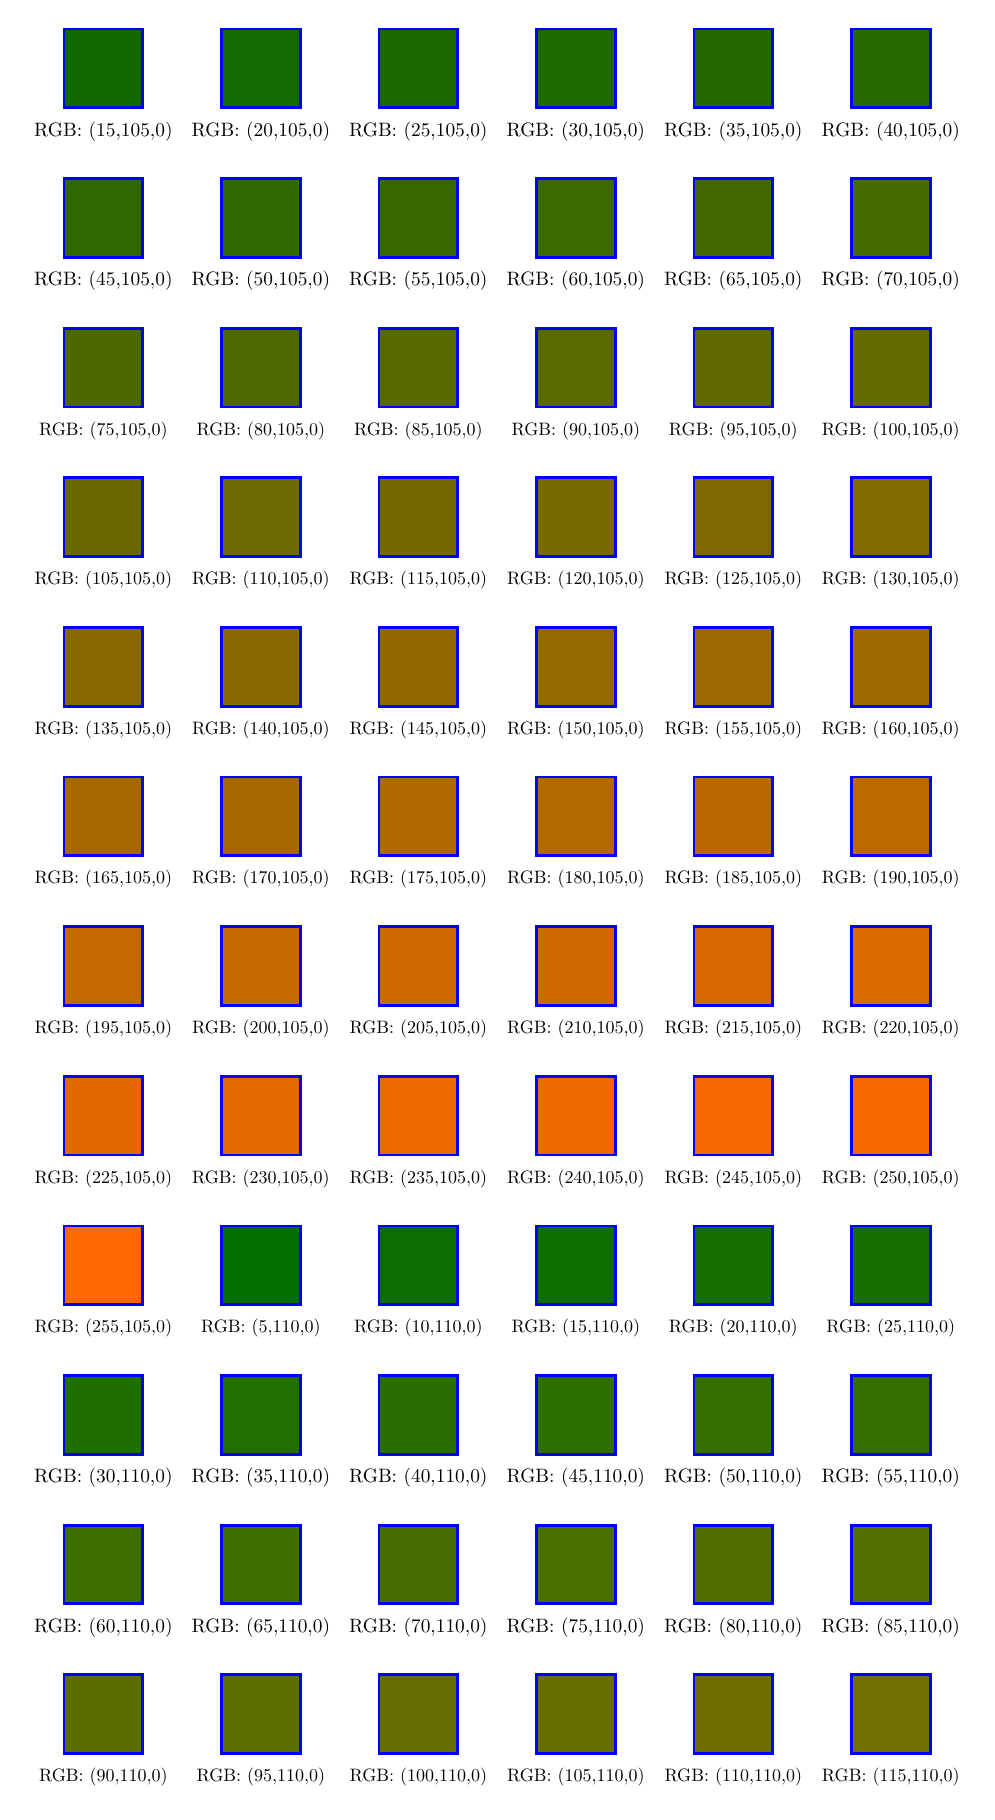
\begin{tikzpicture}

    \filldraw[draw=blue,line width=1,fill=colorR15G105B0]
    (0,0) rectangle (1,1);

    \node[scale=0.7] at (0.5,-0.3) {RGB: (15,105,0)};



    \begin{scope}[xshift=2cm]

      \filldraw[draw=blue,line width=1,fill=colorR20G105B0]
      (0,0) rectangle (1,1);

      \node[scale=0.7] at (0.5,-0.3) {RGB: (20,105,0)};

    \end{scope}



    \begin{scope}[xshift=4cm]

      \filldraw[draw=blue,line width=1,fill=colorR25G105B0]
      (0,0) rectangle (1,1);

      \node[scale=0.7] at (0.5,-0.3) {RGB: (25,105,0)};

    \end{scope}



    \begin{scope}[xshift=6cm]

      \filldraw[draw=blue,line width=1,fill=colorR30G105B0]
      (0,0) rectangle (1,1);

      \node[scale=0.7] at (0.5,-0.3) {RGB: (30,105,0)};

    \end{scope}



    \begin{scope}[xshift=8cm]

      \filldraw[draw=blue,line width=1,fill=colorR35G105B0]
      (0,0) rectangle (1,1);

      \node[scale=0.7] at (0.5,-0.3) {RGB: (35,105,0)};

    \end{scope}



    \begin{scope}[xshift=10cm]

      \filldraw[draw=blue,line width=1,fill=colorR40G105B0]
      (0,0) rectangle (1,1);

      \node[scale=0.7] at (0.5,-0.3) {RGB: (40,105,0)};

    \end{scope}







    \begin{scope}[yshift=-1.9cm]

      \filldraw[draw=blue,line width=1,fill=colorR45G105B0]
      (0,0) rectangle (1,1);

      \node[scale=0.7] at (0.5,-0.3) {RGB: (45,105,0)};

    \end{scope}



    \begin{scope}[xshift=2cm,yshift=-1.9cm]

      \filldraw[draw=blue,line width=1,fill=colorR50G105B0]
      (0,0) rectangle (1,1);

      \node[scale=0.7] at (0.5,-0.3) {RGB: (50,105,0)};

    \end{scope}



    \begin{scope}[xshift=4cm,yshift=-1.9cm]

      \filldraw[draw=blue,line width=1,fill=colorR55G105B0]
      (0,0) rectangle (1,1);

      \node[scale=0.7] at (0.5,-0.3) {RGB: (55,105,0)};

    \end{scope}



    \begin{scope}[xshift=6cm,yshift=-1.9cm]

      \filldraw[draw=blue,line width=1,fill=colorR60G105B0]
      (0,0) rectangle (1,1);

      \node[scale=0.7] at (0.5,-0.3) {RGB: (60,105,0)};

    \end{scope}



    \begin{scope}[xshift=8cm,yshift=-1.9cm]

      \filldraw[draw=blue,line width=1,fill=colorR65G105B0]
      (0,0) rectangle (1,1);

      \node[scale=0.7] at (0.5,-0.3) {RGB: (65,105,0)};

    \end{scope}



    \begin{scope}[xshift=10cm,yshift=-1.9cm]

      \filldraw[draw=blue,line width=1,fill=colorR70G105B0]
      (0,0) rectangle (1,1);

      \node[scale=0.7] at (0.5,-0.3) {RGB: (70,105,0)};

    \end{scope}







    \begin{scope}[yshift=-3.8cm]

      \filldraw[draw=blue,line width=1,fill=colorR75G105B0]
      (0,0) rectangle (1,1);

      \node[scale=0.65] at (0.5,-0.3) {RGB: (75,105,0)};

    \end{scope}



    \begin{scope}[xshift=2cm,yshift=-3.8cm]

      \filldraw[draw=blue,line width=1,fill=colorR80G105B0]
      (0,0) rectangle (1,1);

      \node[scale=0.65] at (0.5,-0.3) {RGB: (80,105,0)};

    \end{scope}



    \begin{scope}[xshift=4cm,yshift=-3.8cm]

      \filldraw[draw=blue,line width=1,fill=colorR85G105B0]
      (0,0) rectangle (1,1);

      \node[scale=0.65] at (0.5,-0.3) {RGB: (85,105,0)};

    \end{scope}



    \begin{scope}[xshift=6cm,yshift=-3.8cm]

      \filldraw[draw=blue,line width=1,fill=colorR90G105B0]
      (0,0) rectangle (1,1);

      \node[scale=0.65] at (0.5,-0.3) {RGB: (90,105,0)};

    \end{scope}



    \begin{scope}[xshift=8cm,yshift=-3.8cm]

      \filldraw[draw=blue,line width=1,fill=colorR95G105B0]
      (0,0) rectangle (1,1);

      \node[scale=0.65] at (0.5,-0.3) {RGB: (95,105,0)};

    \end{scope}



    \begin{scope}[xshift=10cm,yshift=-3.8cm]

      \filldraw[draw=blue,line width=1,fill=colorR100G105B0]
      (0,0) rectangle (1,1);

      \node[scale=0.65] at (0.5,-0.3) {RGB: (100,105,0)};

    \end{scope}







    \begin{scope}[yshift=-5.7cm]

      \filldraw[draw=blue,line width=1,fill=colorR105G105B0]
      (0,0) rectangle (1,1);

      \node[scale=0.65] at (0.5,-0.3) {RGB: (105,105,0)};

    \end{scope}



    \begin{scope}[xshift=2cm,yshift=-5.7cm]

      \filldraw[draw=blue,line width=1,fill=colorR110G105B0]
      (0,0) rectangle (1,1);

      \node[scale=0.65] at (0.5,-0.3) {RGB: (110,105,0)};

    \end{scope}



    \begin{scope}[xshift=4cm,yshift=-5.7cm]

      \filldraw[draw=blue,line width=1,fill=colorR115G105B0]
      (0,0) rectangle (1,1);

      \node[scale=0.65] at (0.5,-0.3) {RGB: (115,105,0)};

    \end{scope}



    \begin{scope}[xshift=6cm,yshift=-5.7cm]

      \filldraw[draw=blue,line width=1,fill=colorR120G105B0]
      (0,0) rectangle (1,1);

      \node[scale=0.65] at (0.5,-0.3) {RGB: (120,105,0)};

    \end{scope}



    \begin{scope}[xshift=8cm,yshift=-5.7cm]

      \filldraw[draw=blue,line width=1,fill=colorR125G105B0]
      (0,0) rectangle (1,1);

      \node[scale=0.65] at (0.5,-0.3) {RGB: (125,105,0)};

    \end{scope}



    \begin{scope}[xshift=10cm,yshift=-5.7cm]

      \filldraw[draw=blue,line width=1,fill=colorR130G105B0]
      (0,0) rectangle (1,1);

      \node[scale=0.65] at (0.5,-0.3) {RGB: (130,105,0)};

    \end{scope}







    \begin{scope}[yshift=-7.6cm]

      \filldraw[draw=blue,line width=1,fill=colorR135G105B0]
      (0,0) rectangle (1,1);

      \node[scale=0.65] at (0.5,-0.3) {RGB: (135,105,0)};

    \end{scope}



    \begin{scope}[xshift=2cm,yshift=-7.6cm]

      \filldraw[draw=blue,line width=1,fill=colorR140G105B0]
      (0,0) rectangle (1,1);

      \node[scale=0.65] at (0.5,-0.3) {RGB: (140,105,0)};

    \end{scope}



    \begin{scope}[xshift=4cm,yshift=-7.6cm]

      \filldraw[draw=blue,line width=1,fill=colorR145G105B0]
      (0,0) rectangle (1,1);

      \node[scale=0.65] at (0.5,-0.3) {RGB: (145,105,0)};

    \end{scope}



    \begin{scope}[xshift=6cm,yshift=-7.6cm]

      \filldraw[draw=blue,line width=1,fill=colorR150G105B0]
      (0,0) rectangle (1,1);

      \node[scale=0.65] at (0.5,-0.3) {RGB: (150,105,0)};

    \end{scope}



    \begin{scope}[xshift=8cm,yshift=-7.6cm]

      \filldraw[draw=blue,line width=1,fill=colorR155G105B0]
      (0,0) rectangle (1,1);

      \node[scale=0.65] at (0.5,-0.3) {RGB: (155,105,0)};

    \end{scope}



    \begin{scope}[xshift=10cm,yshift=-7.6cm]

      \filldraw[draw=blue,line width=1,fill=colorR160G105B0]
      (0,0) rectangle (1,1);

      \node[scale=0.65] at (0.5,-0.3) {RGB: (160,105,0)};

    \end{scope}







    \begin{scope}[yshift=-9.5cm]

      \filldraw[draw=blue,line width=1,fill=colorR165G105B0]
      (0,0) rectangle (1,1);

      \node[scale=0.65] at (0.5,-0.3) {RGB: (165,105,0)};

    \end{scope}



    \begin{scope}[xshift=2cm,yshift=-9.5cm]

      \filldraw[draw=blue,line width=1,fill=colorR170G105B0]
      (0,0) rectangle (1,1);

      \node[scale=0.65] at (0.5,-0.3) {RGB: (170,105,0)};

    \end{scope}



    \begin{scope}[xshift=4cm,yshift=-9.5cm]

      \filldraw[draw=blue,line width=1,fill=colorR175G105B0]
      (0,0) rectangle (1,1);

      \node[scale=0.65] at (0.5,-0.3) {RGB: (175,105,0)};

    \end{scope}



    \begin{scope}[xshift=6cm,yshift=-9.5cm]

      \filldraw[draw=blue,line width=1,fill=colorR180G105B0]
      (0,0) rectangle (1,1);

      \node[scale=0.65] at (0.5,-0.3) {RGB: (180,105,0)};

    \end{scope}



    \begin{scope}[xshift=8cm,yshift=-9.5cm]

      \filldraw[draw=blue,line width=1,fill=colorR185G105B0]
      (0,0) rectangle (1,1);

      \node[scale=0.65] at (0.5,-0.3) {RGB: (185,105,0)};

    \end{scope}



    \begin{scope}[xshift=10cm,yshift=-9.5cm]

      \filldraw[draw=blue,line width=1,fill=colorR190G105B0]
      (0,0) rectangle (1,1);

      \node[scale=0.65] at (0.5,-0.3) {RGB: (190,105,0)};

    \end{scope}







    \begin{scope}[yshift=-11.4cm]

      \filldraw[draw=blue,line width=1,fill=colorR195G105B0]
      (0,0) rectangle (1,1);

      \node[scale=0.65] at (0.5,-0.3) {RGB: (195,105,0)};

    \end{scope}



    \begin{scope}[xshift=2cm,yshift=-11.4cm]

      \filldraw[draw=blue,line width=1,fill=colorR200G105B0]
      (0,0) rectangle (1,1);

      \node[scale=0.65] at (0.5,-0.3) {RGB: (200,105,0)};

    \end{scope}



    \begin{scope}[xshift=4cm,yshift=-11.4cm]

      \filldraw[draw=blue,line width=1,fill=colorR205G105B0]
      (0,0) rectangle (1,1);

      \node[scale=0.65] at (0.5,-0.3) {RGB: (205,105,0)};

    \end{scope}



    \begin{scope}[xshift=6cm,yshift=-11.4cm]

      \filldraw[draw=blue,line width=1,fill=colorR210G105B0]
      (0,0) rectangle (1,1);

      \node[scale=0.65] at (0.5,-0.3) {RGB: (210,105,0)};

    \end{scope}



    \begin{scope}[xshift=8cm,yshift=-11.4cm]

      \filldraw[draw=blue,line width=1,fill=colorR215G105B0]
      (0,0) rectangle (1,1);

      \node[scale=0.65] at (0.5,-0.3) {RGB: (215,105,0)};

    \end{scope}



    \begin{scope}[xshift=10cm,yshift=-11.4cm]

      \filldraw[draw=blue,line width=1,fill=colorR220G105B0]
      (0,0) rectangle (1,1);

      \node[scale=0.65] at (0.5,-0.3) {RGB: (220,105,0)};

    \end{scope}







    \begin{scope}[yshift=-13.3cm]

      \filldraw[draw=blue,line width=1,fill=colorR225G105B0]
      (0,0) rectangle (1,1);

      \node[scale=0.65] at (0.5,-0.3) {RGB: (225,105,0)};

    \end{scope}



    \begin{scope}[xshift=2cm,yshift=-13.3cm]

      \filldraw[draw=blue,line width=1,fill=colorR230G105B0]
      (0,0) rectangle (1,1);

      \node[scale=0.65] at (0.5,-0.3) {RGB: (230,105,0)};

    \end{scope}



    \begin{scope}[xshift=4cm,yshift=-13.3cm]

      \filldraw[draw=blue,line width=1,fill=colorR235G105B0]
      (0,0) rectangle (1,1);

      \node[scale=0.65] at (0.5,-0.3) {RGB: (235,105,0)};

    \end{scope}



    \begin{scope}[xshift=6cm,yshift=-13.3cm]

      \filldraw[draw=blue,line width=1,fill=colorR240G105B0]
      (0,0) rectangle (1,1);

      \node[scale=0.65] at (0.5,-0.3) {RGB: (240,105,0)};

    \end{scope}



    \begin{scope}[xshift=8cm,yshift=-13.3cm]

      \filldraw[draw=blue,line width=1,fill=colorR245G105B0]
      (0,0) rectangle (1,1);

      \node[scale=0.65] at (0.5,-0.3) {RGB: (245,105,0)};

    \end{scope}



    \begin{scope}[xshift=10cm,yshift=-13.3cm]

      \filldraw[draw=blue,line width=1,fill=colorR250G105B0]
      (0,0) rectangle (1,1);

      \node[scale=0.65] at (0.5,-0.3) {RGB: (250,105,0)};

    \end{scope}







    \begin{scope}[yshift=-15.2cm]

      \filldraw[draw=blue,line width=1,fill=colorR255G105B0]
      (0,0) rectangle (1,1);

      \node[scale=0.65] at (0.5,-0.3) {RGB: (255,105,0)};

    \end{scope}



    \begin{scope}[xshift=2cm,yshift=-15.2cm]

      \filldraw[draw=blue,line width=1,fill=colorR5G110B0]
      (0,0) rectangle (1,1);

      \node[scale=0.65] at (0.5,-0.3) {RGB: (5,110,0)};

    \end{scope}



    \begin{scope}[xshift=4cm,yshift=-15.2cm]

      \filldraw[draw=blue,line width=1,fill=colorR10G110B0]
      (0,0) rectangle (1,1);

      \node[scale=0.65] at (0.5,-0.3) {RGB: (10,110,0)};

    \end{scope}



    \begin{scope}[xshift=6cm,yshift=-15.2cm]

      \filldraw[draw=blue,line width=1,fill=colorR15G110B0]
      (0,0) rectangle (1,1);

      \node[scale=0.65] at (0.5,-0.3) {RGB: (15,110,0)};

    \end{scope}



    \begin{scope}[xshift=8cm,yshift=-15.2cm]

      \filldraw[draw=blue,line width=1,fill=colorR20G110B0]
      (0,0) rectangle (1,1);

      \node[scale=0.65] at (0.5,-0.3) {RGB: (20,110,0)};

    \end{scope}



    \begin{scope}[xshift=10cm,yshift=-15.2cm]

      \filldraw[draw=blue,line width=1,fill=colorR25G110B0]
      (0,0) rectangle (1,1);

      \node[scale=0.65] at (0.5,-0.3) {RGB: (25,110,0)};

    \end{scope}







    \begin{scope}[yshift=-17.1cm]

      \filldraw[draw=blue,line width=1,fill=colorR30G110B0]
      (0,0) rectangle (1,1);

      \node[scale=0.7] at (0.5,-0.3) {RGB: (30,110,0)};

    \end{scope}



    \begin{scope}[xshift=2cm,yshift=-17.1cm]

      \filldraw[draw=blue,line width=1,fill=colorR35G110B0]
      (0,0) rectangle (1,1);

      \node[scale=0.7] at (0.5,-0.3) {RGB: (35,110,0)};

    \end{scope}



    \begin{scope}[xshift=4cm,yshift=-17.1cm]

      \filldraw[draw=blue,line width=1,fill=colorR40G110B0]
      (0,0) rectangle (1,1);

      \node[scale=0.7] at (0.5,-0.3) {RGB: (40,110,0)};

    \end{scope}



    \begin{scope}[xshift=6cm,yshift=-17.1cm]

      \filldraw[draw=blue,line width=1,fill=colorR45G110B0]
      (0,0) rectangle (1,1);

      \node[scale=0.7] at (0.5,-0.3) {RGB: (45,110,0)};

    \end{scope}



    \begin{scope}[xshift=8cm,yshift=-17.1cm]

      \filldraw[draw=blue,line width=1,fill=colorR50G110B0]
      (0,0) rectangle (1,1);

      \node[scale=0.7] at (0.5,-0.3) {RGB: (50,110,0)};

    \end{scope}



    \begin{scope}[xshift=10cm,yshift=-17.1cm]

      \filldraw[draw=blue,line width=1,fill=colorR55G110B0]
      (0,0) rectangle (1,1);

      \node[scale=0.7] at (0.5,-0.3) {RGB: (55,110,0)};

    \end{scope}







    \begin{scope}[yshift=-19cm]

      \filldraw[draw=blue,line width=1,fill=colorR60G110B0]
      (0,0) rectangle (1,1);

      \node[scale=0.7] at (0.5,-0.3) {RGB: (60,110,0)};

    \end{scope}



    \begin{scope}[xshift=2cm,yshift=-19cm]

      \filldraw[draw=blue,line width=1,fill=colorR65G110B0]
      (0,0) rectangle (1,1);

      \node[scale=0.7] at (0.5,-0.3) {RGB: (65,110,0)};

    \end{scope}



    \begin{scope}[xshift=4cm,yshift=-19cm]

      \filldraw[draw=blue,line width=1,fill=colorR70G110B0]
      (0,0) rectangle (1,1);

      \node[scale=0.7] at (0.5,-0.3) {RGB: (70,110,0)};

    \end{scope}



    \begin{scope}[xshift=6cm,yshift=-19cm]

      \filldraw[draw=blue,line width=1,fill=colorR75G110B0]
      (0,0) rectangle (1,1);

      \node[scale=0.7] at (0.5,-0.3) {RGB: (75,110,0)};

    \end{scope}



    \begin{scope}[xshift=8cm,yshift=-19cm]

      \filldraw[draw=blue,line width=1,fill=colorR80G110B0]
      (0,0) rectangle (1,1);

      \node[scale=0.7] at (0.5,-0.3) {RGB: (80,110,0)};

    \end{scope}



    \begin{scope}[xshift=10cm,yshift=-19cm]

      \filldraw[draw=blue,line width=1,fill=colorR85G110B0]
      (0,0) rectangle (1,1);

      \node[scale=0.7] at (0.5,-0.3) {RGB: (85,110,0)};

    \end{scope}







    \begin{scope}[yshift=-20.9cm]

      \filldraw[draw=blue,line width=1,fill=colorR90G110B0]
      (0,0) rectangle (1,1);

      \node[scale=0.65] at (0.5,-0.3) {RGB: (90,110,0)};

    \end{scope}



    \begin{scope}[xshift=2cm,yshift=-20.9cm]

      \filldraw[draw=blue,line width=1,fill=colorR95G110B0]
      (0,0) rectangle (1,1);

      \node[scale=0.65] at (0.5,-0.3) {RGB: (95,110,0)};

    \end{scope}



    \begin{scope}[xshift=4cm,yshift=-20.9cm]

      \filldraw[draw=blue,line width=1,fill=colorR100G110B0]
      (0,0) rectangle (1,1);

      \node[scale=0.65] at (0.5,-0.3) {RGB: (100,110,0)};

    \end{scope}



    \begin{scope}[xshift=6cm,yshift=-20.9cm]

      \filldraw[draw=blue,line width=1,fill=colorR105G110B0]
      (0,0) rectangle (1,1);

      \node[scale=0.65] at (0.5,-0.3) {RGB: (105,110,0)};

    \end{scope}



    \begin{scope}[xshift=8cm,yshift=-20.9cm]

      \filldraw[draw=blue,line width=1,fill=colorR110G110B0]
      (0,0) rectangle (1,1);

      \node[scale=0.65] at (0.5,-0.3) {RGB: (110,110,0)};

    \end{scope}



    \begin{scope}[xshift=10cm,yshift=-20.9cm]

      \filldraw[draw=blue,line width=1,fill=colorR115G110B0]
      (0,0) rectangle (1,1);

      \node[scale=0.65] at (0.5,-0.3) {RGB: (115,110,0)};

    \end{scope}

  \end{tikzpicture}

  \caption{Mixed colors in~RGB system: $(15,105,0)$--$(255,105,0)$,
    $(5,110,0)$--$(115,110,0)$}



  \label{fig:Mixed-colors-Part-06}

\end{figure}
% ##################





% ##################
\begin{figure}

  \centering


  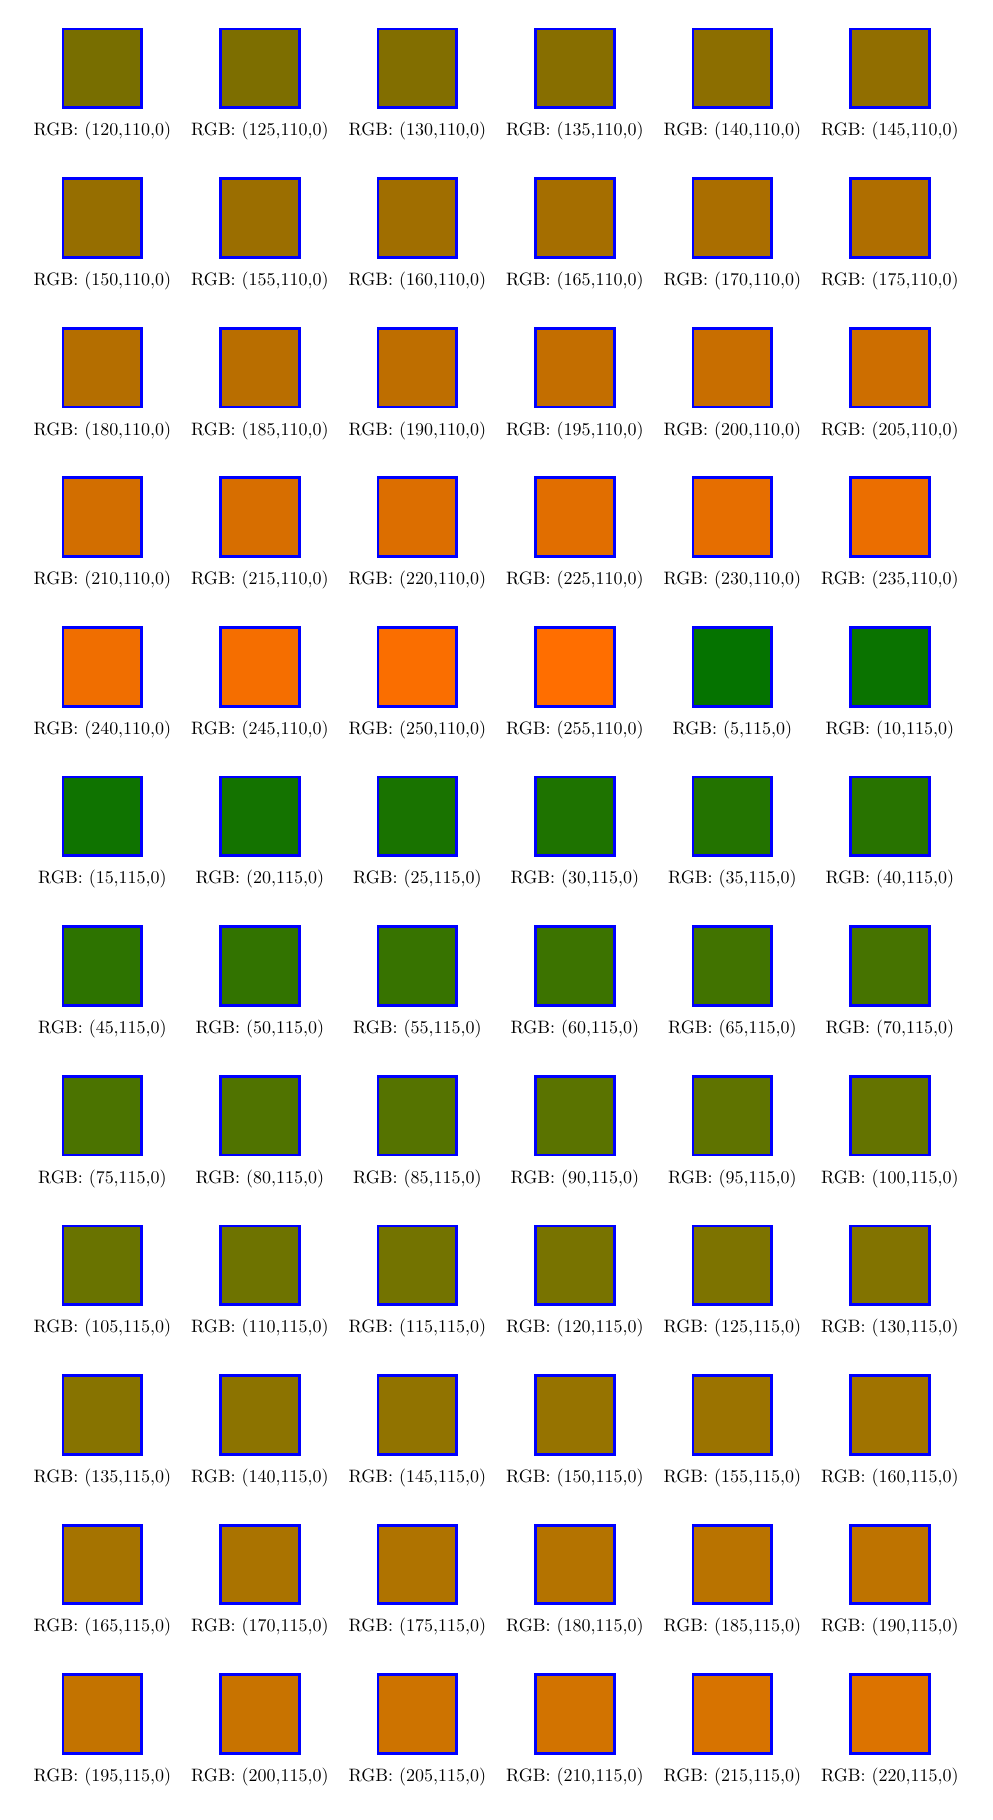
\begin{tikzpicture}

    \filldraw[draw=blue,line width=1,fill=colorR120G110B0]
    (0,0) rectangle (1,1);

    \node[scale=0.65] at (0.5,-0.3) {RGB: (120,110,0)};



    \begin{scope}[xshift=2cm]

      \filldraw[draw=blue,line width=1,fill=colorR125G110B0]
      (0,0) rectangle (1,1);

      \node[scale=0.65] at (0.5,-0.3) {RGB: (125,110,0)};

    \end{scope}



    \begin{scope}[xshift=4cm]

      \filldraw[draw=blue,line width=1,fill=colorR130G110B0]
      (0,0) rectangle (1,1);

      \node[scale=0.65] at (0.5,-0.3) {RGB: (130,110,0)};

    \end{scope}



    \begin{scope}[xshift=6cm]

      \filldraw[draw=blue,line width=1,fill=colorR135G110B0]
      (0,0) rectangle (1,1);

      \node[scale=0.65] at (0.5,-0.3) {RGB: (135,110,0)};

    \end{scope}



    \begin{scope}[xshift=8cm]

      \filldraw[draw=blue,line width=1,fill=colorR140G110B0]
      (0,0) rectangle (1,1);

      \node[scale=0.65] at (0.5,-0.3) {RGB: (140,110,0)};

    \end{scope}



    \begin{scope}[xshift=10cm]

      \filldraw[draw=blue,line width=1,fill=colorR145G110B0]
      (0,0) rectangle (1,1);

      \node[scale=0.65] at (0.5,-0.3) {RGB: (145,110,0)};

    \end{scope}







    \begin{scope}[yshift=-1.9cm]

      \filldraw[draw=blue,line width=1,fill=colorR150G110B0]
      (0,0) rectangle (1,1);

      \node[scale=0.65] at (0.5,-0.3) {RGB: (150,110,0)};

    \end{scope}



    \begin{scope}[xshift=2cm,yshift=-1.9cm]

      \filldraw[draw=blue,line width=1,fill=colorR155G110B0]
      (0,0) rectangle (1,1);

      \node[scale=0.65] at (0.5,-0.3) {RGB: (155,110,0)};

    \end{scope}



    \begin{scope}[xshift=4cm,yshift=-1.9cm]

      \filldraw[draw=blue,line width=1,fill=colorR160G110B0]
      (0,0) rectangle (1,1);

      \node[scale=0.65] at (0.5,-0.3) {RGB: (160,110,0)};

    \end{scope}



    \begin{scope}[xshift=6cm,yshift=-1.9cm]

      \filldraw[draw=blue,line width=1,fill=colorR165G110B0]
      (0,0) rectangle (1,1);

      \node[scale=0.65] at (0.5,-0.3) {RGB: (165,110,0)};

    \end{scope}



    \begin{scope}[xshift=8cm,yshift=-1.9cm]

      \filldraw[draw=blue,line width=1,fill=colorR170G110B0]
      (0,0) rectangle (1,1);

      \node[scale=0.65] at (0.5,-0.3) {RGB: (170,110,0)};

    \end{scope}



    \begin{scope}[xshift=10cm,yshift=-1.9cm]

      \filldraw[draw=blue,line width=1,fill=colorR175G110B0]
      (0,0) rectangle (1,1);

      \node[scale=0.65] at (0.5,-0.3) {RGB: (175,110,0)};

    \end{scope}







    \begin{scope}[yshift=-3.8cm]

      \filldraw[draw=blue,line width=1,fill=colorR180G110B0]
      (0,0) rectangle (1,1);

      \node[scale=0.65] at (0.5,-0.3) {RGB: (180,110,0)};

    \end{scope}



    \begin{scope}[xshift=2cm,yshift=-3.8cm]

      \filldraw[draw=blue,line width=1,fill=colorR185G110B0]
      (0,0) rectangle (1,1);

      \node[scale=0.65] at (0.5,-0.3) {RGB: (185,110,0)};

    \end{scope}



    \begin{scope}[xshift=4cm,yshift=-3.8cm]

      \filldraw[draw=blue,line width=1,fill=colorR190G110B0]
      (0,0) rectangle (1,1);

      \node[scale=0.65] at (0.5,-0.3) {RGB: (190,110,0)};

    \end{scope}



    \begin{scope}[xshift=6cm,yshift=-3.8cm]

      \filldraw[draw=blue,line width=1,fill=colorR195G110B0]
      (0,0) rectangle (1,1);

      \node[scale=0.65] at (0.5,-0.3) {RGB: (195,110,0)};

    \end{scope}



    \begin{scope}[xshift=8cm,yshift=-3.8cm]

      \filldraw[draw=blue,line width=1,fill=colorR200G110B0]
      (0,0) rectangle (1,1);

      \node[scale=0.65] at (0.5,-0.3) {RGB: (200,110,0)};

    \end{scope}



    \begin{scope}[xshift=10cm,yshift=-3.8cm]

      \filldraw[draw=blue,line width=1,fill=colorR205G110B0]
      (0,0) rectangle (1,1);

      \node[scale=0.65] at (0.5,-0.3) {RGB: (205,110,0)};

    \end{scope}







    \begin{scope}[yshift=-5.7cm]

      \filldraw[draw=blue,line width=1,fill=colorR210G110B0]
      (0,0) rectangle (1,1);

      \node[scale=0.65] at (0.5,-0.3) {RGB: (210,110,0)};

    \end{scope}



    \begin{scope}[xshift=2cm,yshift=-5.7cm]

      \filldraw[draw=blue,line width=1,fill=colorR215G110B0]
      (0,0) rectangle (1,1);

      \node[scale=0.65] at (0.5,-0.3) {RGB: (215,110,0)};

    \end{scope}



    \begin{scope}[xshift=4cm,yshift=-5.7cm]

      \filldraw[draw=blue,line width=1,fill=colorR220G110B0]
      (0,0) rectangle (1,1);

      \node[scale=0.65] at (0.5,-0.3) {RGB: (220,110,0)};

    \end{scope}



    \begin{scope}[xshift=6cm,yshift=-5.7cm]

      \filldraw[draw=blue,line width=1,fill=colorR225G110B0]
      (0,0) rectangle (1,1);

      \node[scale=0.65] at (0.5,-0.3) {RGB: (225,110,0)};

    \end{scope}



    \begin{scope}[xshift=8cm,yshift=-5.7cm]

      \filldraw[draw=blue,line width=1,fill=colorR230G110B0]
      (0,0) rectangle (1,1);

      \node[scale=0.65] at (0.5,-0.3) {RGB: (230,110,0)};

    \end{scope}



    \begin{scope}[xshift=10cm,yshift=-5.7cm]

      \filldraw[draw=blue,line width=1,fill=colorR235G110B0]
      (0,0) rectangle (1,1);

      \node[scale=0.65] at (0.5,-0.3) {RGB: (235,110,0)};

    \end{scope}







    \begin{scope}[yshift=-7.6cm]

      \filldraw[draw=blue,line width=1,fill=colorR240G110B0]
      (0,0) rectangle (1,1);

      \node[scale=0.65] at (0.5,-0.3) {RGB: (240,110,0)};

    \end{scope}



    \begin{scope}[xshift=2cm,yshift=-7.6cm]

      \filldraw[draw=blue,line width=1,fill=colorR245G110B0]
      (0,0) rectangle (1,1);

      \node[scale=0.65] at (0.5,-0.3) {RGB: (245,110,0)};

    \end{scope}



    \begin{scope}[xshift=4cm,yshift=-7.6cm]

      \filldraw[draw=blue,line width=1,fill=colorR250G110B0]
      (0,0) rectangle (1,1);

      \node[scale=0.65] at (0.5,-0.3) {RGB: (250,110,0)};

    \end{scope}



    \begin{scope}[xshift=6cm,yshift=-7.6cm]

      \filldraw[draw=blue,line width=1,fill=colorR255G110B0]
      (0,0) rectangle (1,1);

      \node[scale=0.65] at (0.5,-0.3) {RGB: (255,110,0)};

    \end{scope}



    \begin{scope}[xshift=8cm,yshift=-7.6cm]

      \filldraw[draw=blue,line width=1,fill=colorR5G115B0]
      (0,0) rectangle (1,1);

      \node[scale=0.65] at (0.5,-0.3) {RGB: (5,115,0)};

    \end{scope}



    \begin{scope}[xshift=10cm,yshift=-7.6cm]

      \filldraw[draw=blue,line width=1,fill=colorR10G115B0]
      (0,0) rectangle (1,1);

      \node[scale=0.65] at (0.5,-0.3) {RGB: (10,115,0)};

    \end{scope}







    \begin{scope}[yshift=-9.5cm]

      \filldraw[draw=blue,line width=1,fill=colorR15G115B0]
      (0,0) rectangle (1,1);

      \node[scale=0.65] at (0.5,-0.3) {RGB: (15,115,0)};

    \end{scope}



    \begin{scope}[xshift=2cm,yshift=-9.5cm]

      \filldraw[draw=blue,line width=1,fill=colorR20G115B0]
      (0,0) rectangle (1,1);

      \node[scale=0.65] at (0.5,-0.3) {RGB: (20,115,0)};

    \end{scope}



    \begin{scope}[xshift=4cm,yshift=-9.5cm]

      \filldraw[draw=blue,line width=1,fill=colorR25G115B0]
      (0,0) rectangle (1,1);

      \node[scale=0.65] at (0.5,-0.3) {RGB: (25,115,0)};

    \end{scope}



    \begin{scope}[xshift=6cm,yshift=-9.5cm]

      \filldraw[draw=blue,line width=1,fill=colorR30G115B0]
      (0,0) rectangle (1,1);

      \node[scale=0.65] at (0.5,-0.3) {RGB: (30,115,0)};

    \end{scope}



    \begin{scope}[xshift=8cm,yshift=-9.5cm]

      \filldraw[draw=blue,line width=1,fill=colorR35G115B0]
      (0,0) rectangle (1,1);

      \node[scale=0.65] at (0.5,-0.3) {RGB: (35,115,0)};

    \end{scope}



    \begin{scope}[xshift=10cm,yshift=-9.5cm]

      \filldraw[draw=blue,line width=1,fill=colorR40G115B0]
      (0,0) rectangle (1,1);

      \node[scale=0.65] at (0.5,-0.3) {RGB: (40,115,0)};

    \end{scope}







    \begin{scope}[yshift=-11.4cm]

      \filldraw[draw=blue,line width=1,fill=colorR45G115B0]
      (0,0) rectangle (1,1);

      \node[scale=0.65] at (0.5,-0.3) {RGB: (45,115,0)};

    \end{scope}



    \begin{scope}[xshift=2cm,yshift=-11.4cm]

      \filldraw[draw=blue,line width=1,fill=colorR50G115B0]
      (0,0) rectangle (1,1);

      \node[scale=0.65] at (0.5,-0.3) {RGB: (50,115,0)};

    \end{scope}



    \begin{scope}[xshift=4cm,yshift=-11.4cm]

      \filldraw[draw=blue,line width=1,fill=colorR55G115B0]
      (0,0) rectangle (1,1);

      \node[scale=0.65] at (0.5,-0.3) {RGB: (55,115,0)};

    \end{scope}



    \begin{scope}[xshift=6cm,yshift=-11.4cm]

      \filldraw[draw=blue,line width=1,fill=colorR60G115B0]
      (0,0) rectangle (1,1);

      \node[scale=0.65] at (0.5,-0.3) {RGB: (60,115,0)};

    \end{scope}



    \begin{scope}[xshift=8cm,yshift=-11.4cm]

      \filldraw[draw=blue,line width=1,fill=colorR65G115B0]
      (0,0) rectangle (1,1);

      \node[scale=0.65] at (0.5,-0.3) {RGB: (65,115,0)};

    \end{scope}



    \begin{scope}[xshift=10cm,yshift=-11.4cm]

      \filldraw[draw=blue,line width=1,fill=colorR70G115B0]
      (0,0) rectangle (1,1);

      \node[scale=0.65] at (0.5,-0.3) {RGB: (70,115,0)};

    \end{scope}







    \begin{scope}[yshift=-13.3cm]

      \filldraw[draw=blue,line width=1,fill=colorR75G115B0]
      (0,0) rectangle (1,1);

      \node[scale=0.65] at (0.5,-0.3) {RGB: (75,115,0)};

    \end{scope}



    \begin{scope}[xshift=2cm,yshift=-13.3cm]

      \filldraw[draw=blue,line width=1,fill=colorR80G115B0]
      (0,0) rectangle (1,1);

      \node[scale=0.65] at (0.5,-0.3) {RGB: (80,115,0)};

    \end{scope}



    \begin{scope}[xshift=4cm,yshift=-13.3cm]

      \filldraw[draw=blue,line width=1,fill=colorR85G115B0]
      (0,0) rectangle (1,1);

      \node[scale=0.65] at (0.5,-0.3) {RGB: (85,115,0)};

    \end{scope}



    \begin{scope}[xshift=6cm,yshift=-13.3cm]

      \filldraw[draw=blue,line width=1,fill=colorR90G115B0]
      (0,0) rectangle (1,1);

      \node[scale=0.65] at (0.5,-0.3) {RGB: (90,115,0)};

    \end{scope}



    \begin{scope}[xshift=8cm,yshift=-13.3cm]

      \filldraw[draw=blue,line width=1,fill=colorR95G115B0]
      (0,0) rectangle (1,1);

      \node[scale=0.65] at (0.5,-0.3) {RGB: (95,115,0)};

    \end{scope}



    \begin{scope}[xshift=10cm,yshift=-13.3cm]

      \filldraw[draw=blue,line width=1,fill=colorR100G115B0]
      (0,0) rectangle (1,1);

      \node[scale=0.65] at (0.5,-0.3) {RGB: (100,115,0)};

    \end{scope}







    \begin{scope}[yshift=-15.2cm]

      \filldraw[draw=blue,line width=1,fill=colorR105G115B0]
      (0,0) rectangle (1,1);

      \node[scale=0.65] at (0.5,-0.3) {RGB: (105,115,0)};

    \end{scope}



    \begin{scope}[xshift=2cm,yshift=-15.2cm]

      \filldraw[draw=blue,line width=1,fill=colorR110G115B0]
      (0,0) rectangle (1,1);

      \node[scale=0.65] at (0.5,-0.3) {RGB: (110,115,0)};

    \end{scope}



    \begin{scope}[xshift=4cm,yshift=-15.2cm]

      \filldraw[draw=blue,line width=1,fill=colorR115G115B0]
      (0,0) rectangle (1,1);

      \node[scale=0.65] at (0.5,-0.3) {RGB: (115,115,0)};

    \end{scope}



    \begin{scope}[xshift=6cm,yshift=-15.2cm]

      \filldraw[draw=blue,line width=1,fill=colorR120G115B0]
      (0,0) rectangle (1,1);

      \node[scale=0.65] at (0.5,-0.3) {RGB: (120,115,0)};

    \end{scope}



    \begin{scope}[xshift=8cm,yshift=-15.2cm]

      \filldraw[draw=blue,line width=1,fill=colorR125G115B0]
      (0,0) rectangle (1,1);

      \node[scale=0.65] at (0.5,-0.3) {RGB: (125,115,0)};

    \end{scope}



    \begin{scope}[xshift=10cm,yshift=-15.2cm]

      \filldraw[draw=blue,line width=1,fill=colorR130G115B0]
      (0,0) rectangle (1,1);

      \node[scale=0.65] at (0.5,-0.3) {RGB: (130,115,0)};

    \end{scope}







    \begin{scope}[yshift=-17.1cm]

      \filldraw[draw=blue,line width=1,fill=colorR135G115B0]
      (0,0) rectangle (1,1);

      \node[scale=0.65] at (0.5,-0.3) {RGB: (135,115,0)};

    \end{scope}



    \begin{scope}[xshift=2cm,yshift=-17.1cm]

      \filldraw[draw=blue,line width=1,fill=colorR140G115B0]
      (0,0) rectangle (1,1);

      \node[scale=0.65] at (0.5,-0.3) {RGB: (140,115,0)};

    \end{scope}



    \begin{scope}[xshift=4cm,yshift=-17.1cm]

      \filldraw[draw=blue,line width=1,fill=colorR145G115B0]
      (0,0) rectangle (1,1);

      \node[scale=0.65] at (0.5,-0.3) {RGB: (145,115,0)};

    \end{scope}



    \begin{scope}[xshift=6cm,yshift=-17.1cm]

      \filldraw[draw=blue,line width=1,fill=colorR150G115B0]
      (0,0) rectangle (1,1);

      \node[scale=0.65] at (0.5,-0.3) {RGB: (150,115,0)};

    \end{scope}



    \begin{scope}[xshift=8cm,yshift=-17.1cm]

      \filldraw[draw=blue,line width=1,fill=colorR155G115B0]
      (0,0) rectangle (1,1);

      \node[scale=0.65] at (0.5,-0.3) {RGB: (155,115,0)};

    \end{scope}



    \begin{scope}[xshift=10cm,yshift=-17.1cm]

      \filldraw[draw=blue,line width=1,fill=colorR160G115B0]
      (0,0) rectangle (1,1);

      \node[scale=0.65] at (0.5,-0.3) {RGB: (160,115,0)};

    \end{scope}







    \begin{scope}[yshift=-19cm]

      \filldraw[draw=blue,line width=1,fill=colorR165G115B0]
      (0,0) rectangle (1,1);

      \node[scale=0.65] at (0.5,-0.3) {RGB: (165,115,0)};

    \end{scope}



    \begin{scope}[xshift=2cm,yshift=-19cm]

      \filldraw[draw=blue,line width=1,fill=colorR170G115B0]
      (0,0) rectangle (1,1);

      \node[scale=0.65] at (0.5,-0.3) {RGB: (170,115,0)};

    \end{scope}



    \begin{scope}[xshift=4cm,yshift=-19cm]

      \filldraw[draw=blue,line width=1,fill=colorR175G115B0]
      (0,0) rectangle (1,1);

      \node[scale=0.65] at (0.5,-0.3) {RGB: (175,115,0)};

    \end{scope}



    \begin{scope}[xshift=6cm,yshift=-19cm]

      \filldraw[draw=blue,line width=1,fill=colorR180G115B0]
      (0,0) rectangle (1,1);

      \node[scale=0.65] at (0.5,-0.3) {RGB: (180,115,0)};

    \end{scope}



    \begin{scope}[xshift=8cm,yshift=-19cm]

      \filldraw[draw=blue,line width=1,fill=colorR185G115B0]
      (0,0) rectangle (1,1);

      \node[scale=0.65] at (0.5,-0.3) {RGB: (185,115,0)};

    \end{scope}



    \begin{scope}[xshift=10cm,yshift=-19cm]

      \filldraw[draw=blue,line width=1,fill=colorR190G115B0]
      (0,0) rectangle (1,1);

      \node[scale=0.65] at (0.5,-0.3) {RGB: (190,115,0)};

    \end{scope}







    \begin{scope}[yshift=-20.9cm]

      \filldraw[draw=blue,line width=1,fill=colorR195G115B0]
      (0,0) rectangle (1,1);

      \node[scale=0.65] at (0.5,-0.3) {RGB: (195,115,0)};

    \end{scope}



    \begin{scope}[xshift=2cm,yshift=-20.9cm]

      \filldraw[draw=blue,line width=1,fill=colorR200G115B0]
      (0,0) rectangle (1,1);

      \node[scale=0.65] at (0.5,-0.3) {RGB: (200,115,0)};

    \end{scope}



    \begin{scope}[xshift=4cm,yshift=-20.9cm]

      \filldraw[draw=blue,line width=1,fill=colorR205G115B0]
      (0,0) rectangle (1,1);

      \node[scale=0.65] at (0.5,-0.3) {RGB: (205,115,0)};

    \end{scope}



    \begin{scope}[xshift=6cm,yshift=-20.9cm]

      \filldraw[draw=blue,line width=1,fill=colorR210G115B0]
      (0,0) rectangle (1,1);

      \node[scale=0.65] at (0.5,-0.3) {RGB: (210,115,0)};

    \end{scope}



    \begin{scope}[xshift=8cm,yshift=-20.9cm]

      \filldraw[draw=blue,line width=1,fill=colorR215G115B0]
      (0,0) rectangle (1,1);

      \node[scale=0.65] at (0.5,-0.3) {RGB: (215,115,0)};

    \end{scope}



    \begin{scope}[xshift=10cm,yshift=-20.9cm]

      \filldraw[draw=blue,line width=1,fill=colorR220G115B0]
      (0,0) rectangle (1,1);

      \node[scale=0.65] at (0.5,-0.3) {RGB: (220,115,0)};

    \end{scope}

  \end{tikzpicture}

  \caption{Mixed colors in~RGB system: $(120,110,0)$--$(255,110,0)$,
    $(5,115,0)$--$(220,115,0)$}



  \label{fig:Mixed-colors-Part-07}

\end{figure}
% ##################





% ##################
\begin{figure}

  \centering


  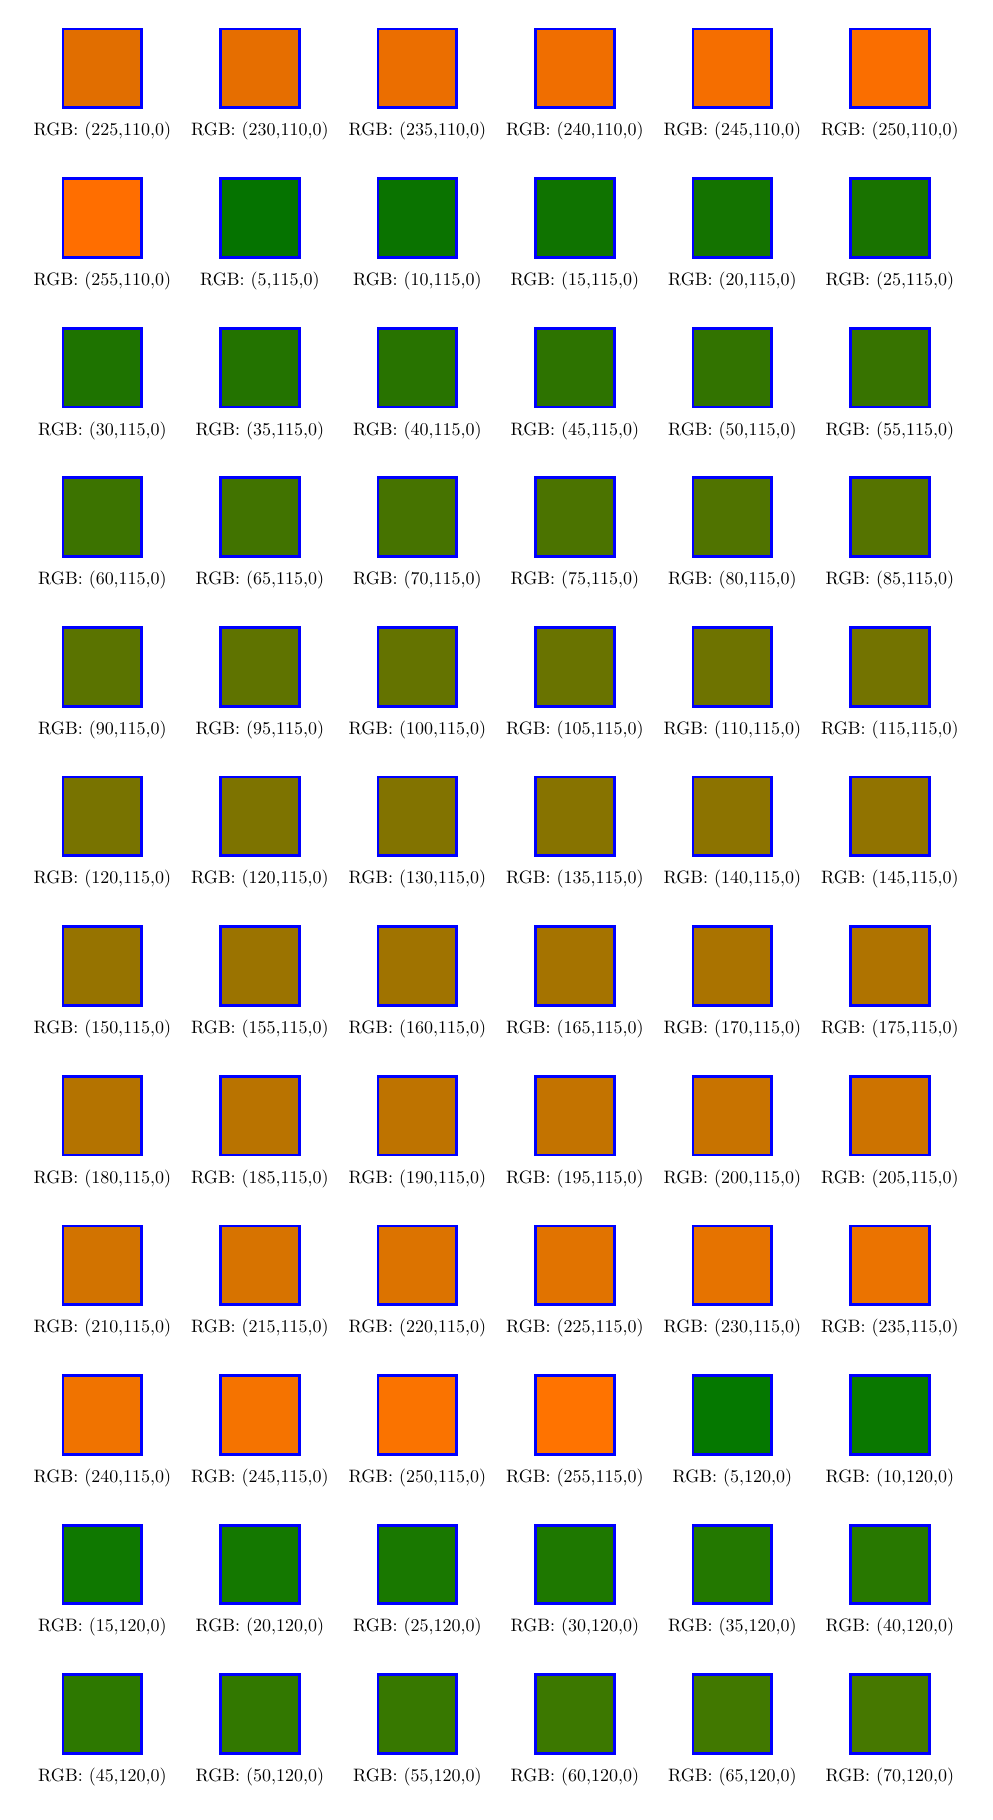
\begin{tikzpicture}

    \filldraw[draw=blue,line width=1,fill=colorR225G110B0]
    (0,0) rectangle (1,1);

    \node[scale=0.65] at (0.5,-0.3) {RGB: (225,110,0)};



    \begin{scope}[xshift=2cm]

      \filldraw[draw=blue,line width=1,fill=colorR230G110B0]
      (0,0) rectangle (1,1);

      \node[scale=0.65] at (0.5,-0.3) {RGB: (230,110,0)};

    \end{scope}



    \begin{scope}[xshift=4cm]

      \filldraw[draw=blue,line width=1,fill=colorR235G110B0]
      (0,0) rectangle (1,1);

      \node[scale=0.65] at (0.5,-0.3) {RGB: (235,110,0)};

    \end{scope}



    \begin{scope}[xshift=6cm]

      \filldraw[draw=blue,line width=1,fill=colorR240G110B0]
      (0,0) rectangle (1,1);

      \node[scale=0.65] at (0.5,-0.3) {RGB: (240,110,0)};

    \end{scope}



    \begin{scope}[xshift=8cm]

      \filldraw[draw=blue,line width=1,fill=colorR245G110B0]
      (0,0) rectangle (1,1);

      \node[scale=0.65] at (0.5,-0.3) {RGB: (245,110,0)};

    \end{scope}



    \begin{scope}[xshift=10cm]

      \filldraw[draw=blue,line width=1,fill=colorR250G110B0]
      (0,0) rectangle (1,1);

      \node[scale=0.65] at (0.5,-0.3) {RGB: (250,110,0)};

    \end{scope}







    \begin{scope}[yshift=-1.9cm]

      \filldraw[draw=blue,line width=1,fill=colorR255G110B0]
      (0,0) rectangle (1,1);

      \node[scale=0.65] at (0.5,-0.3) {RGB: (255,110,0)};

    \end{scope}



    \begin{scope}[xshift=2cm,yshift=-1.9cm]

      \filldraw[draw=blue,line width=1,fill=colorR5G115B0]
      (0,0) rectangle (1,1);

      \node[scale=0.65] at (0.5,-0.3) {RGB: (5,115,0)};

    \end{scope}



    \begin{scope}[xshift=4cm,yshift=-1.9cm]

      \filldraw[draw=blue,line width=1,fill=colorR10G115B0]
      (0,0) rectangle (1,1);

      \node[scale=0.65] at (0.5,-0.3) {RGB: (10,115,0)};

    \end{scope}



    \begin{scope}[xshift=6cm,yshift=-1.9cm]

      \filldraw[draw=blue,line width=1,fill=colorR15G115B0]
      (0,0) rectangle (1,1);

      \node[scale=0.65] at (0.5,-0.3) {RGB: (15,115,0)};

    \end{scope}



    \begin{scope}[xshift=8cm,yshift=-1.9cm]

      \filldraw[draw=blue,line width=1,fill=colorR20G115B0]
      (0,0) rectangle (1,1);

      \node[scale=0.65] at (0.5,-0.3) {RGB: (20,115,0)};

    \end{scope}



    \begin{scope}[xshift=10cm,yshift=-1.9cm]

      \filldraw[draw=blue,line width=1,fill=colorR25G115B0]
      (0,0) rectangle (1,1);

      \node[scale=0.65] at (0.5,-0.3) {RGB: (25,115,0)};

    \end{scope}







    \begin{scope}[yshift=-3.8cm]

      \filldraw[draw=blue,line width=1,fill=colorR30G115B0]
      (0,0) rectangle (1,1);

      \node[scale=0.65] at (0.5,-0.3) {RGB: (30,115,0)};

    \end{scope}



    \begin{scope}[xshift=2cm,yshift=-3.8cm]

      \filldraw[draw=blue,line width=1,fill=colorR35G115B0]
      (0,0) rectangle (1,1);

      \node[scale=0.65] at (0.5,-0.3) {RGB: (35,115,0)};

    \end{scope}



    \begin{scope}[xshift=4cm,yshift=-3.8cm]

      \filldraw[draw=blue,line width=1,fill=colorR40G115B0]
      (0,0) rectangle (1,1);

      \node[scale=0.65] at (0.5,-0.3) {RGB: (40,115,0)};

    \end{scope}



    \begin{scope}[xshift=6cm,yshift=-3.8cm]

      \filldraw[draw=blue,line width=1,fill=colorR45G115B0]
      (0,0) rectangle (1,1);

      \node[scale=0.65] at (0.5,-0.3) {RGB: (45,115,0)};

    \end{scope}



    \begin{scope}[xshift=8cm,yshift=-3.8cm]

      \filldraw[draw=blue,line width=1,fill=colorR50G115B0]
      (0,0) rectangle (1,1);

      \node[scale=0.65] at (0.5,-0.3) {RGB: (50,115,0)};

    \end{scope}



    \begin{scope}[xshift=10cm,yshift=-3.8cm]

      \filldraw[draw=blue,line width=1,fill=colorR55G115B0]
      (0,0) rectangle (1,1);

      \node[scale=0.65] at (0.5,-0.3) {RGB: (55,115,0)};

    \end{scope}







    \begin{scope}[yshift=-5.7cm]

      \filldraw[draw=blue,line width=1,fill=colorR60G115B0]
      (0,0) rectangle (1,1);

      \node[scale=0.65] at (0.5,-0.3) {RGB: (60,115,0)};

    \end{scope}



    \begin{scope}[xshift=2cm,yshift=-5.7cm]

      \filldraw[draw=blue,line width=1,fill=colorR65G115B0]
      (0,0) rectangle (1,1);

      \node[scale=0.65] at (0.5,-0.3) {RGB: (65,115,0)};

    \end{scope}



    \begin{scope}[xshift=4cm,yshift=-5.7cm]

      \filldraw[draw=blue,line width=1,fill=colorR70G115B0]
      (0,0) rectangle (1,1);

      \node[scale=0.65] at (0.5,-0.3) {RGB: (70,115,0)};

    \end{scope}



    \begin{scope}[xshift=6cm,yshift=-5.7cm]

      \filldraw[draw=blue,line width=1,fill=colorR75G115B0]
      (0,0) rectangle (1,1);

      \node[scale=0.65] at (0.5,-0.3) {RGB: (75,115,0)};

    \end{scope}



    \begin{scope}[xshift=8cm,yshift=-5.7cm]

      \filldraw[draw=blue,line width=1,fill=colorR80G115B0]
      (0,0) rectangle (1,1);

      \node[scale=0.65] at (0.5,-0.3) {RGB: (80,115,0)};

    \end{scope}



    \begin{scope}[xshift=10cm,yshift=-5.7cm]

      \filldraw[draw=blue,line width=1,fill=colorR85G115B0]
      (0,0) rectangle (1,1);

      \node[scale=0.65] at (0.5,-0.3) {RGB: (85,115,0)};

    \end{scope}







    \begin{scope}[yshift=-7.6cm]

      \filldraw[draw=blue,line width=1,fill=colorR90G115B0]
      (0,0) rectangle (1,1);

      \node[scale=0.65] at (0.5,-0.3) {RGB: (90,115,0)};

    \end{scope}



    \begin{scope}[xshift=2cm,yshift=-7.6cm]

      \filldraw[draw=blue,line width=1,fill=colorR95G115B0]
      (0,0) rectangle (1,1);

      \node[scale=0.65] at (0.5,-0.3) {RGB: (95,115,0)};

    \end{scope}



    \begin{scope}[xshift=4cm,yshift=-7.6cm]

      \filldraw[draw=blue,line width=1,fill=colorR100G115B0]
      (0,0) rectangle (1,1);

      \node[scale=0.65] at (0.5,-0.3) {RGB: (100,115,0)};

    \end{scope}



    \begin{scope}[xshift=6cm,yshift=-7.6cm]

      \filldraw[draw=blue,line width=1,fill=colorR105G115B0]
      (0,0) rectangle (1,1);

      \node[scale=0.65] at (0.5,-0.3) {RGB: (105,115,0)};

    \end{scope}



    \begin{scope}[xshift=8cm,yshift=-7.6cm]

      \filldraw[draw=blue,line width=1,fill=colorR110G115B0]
      (0,0) rectangle (1,1);

      \node[scale=0.65] at (0.5,-0.3) {RGB: (110,115,0)};

    \end{scope}



    \begin{scope}[xshift=10cm,yshift=-7.6cm]

      \filldraw[draw=blue,line width=1,fill=colorR115G115B0]
      (0,0) rectangle (1,1);

      \node[scale=0.65] at (0.5,-0.3) {RGB: (115,115,0)};

    \end{scope}







    \begin{scope}[yshift=-9.5cm]

      \filldraw[draw=blue,line width=1,fill=colorR120G115B0]
      (0,0) rectangle (1,1);

      \node[scale=0.65] at (0.5,-0.3) {RGB: (120,115,0)};

    \end{scope}



    \begin{scope}[xshift=2cm,yshift=-9.5cm]

      \filldraw[draw=blue,line width=1,fill=colorR125G115B0]
      (0,0) rectangle (1,1);

      \node[scale=0.65] at (0.5,-0.3) {RGB: (120,115,0)};

    \end{scope}



    \begin{scope}[xshift=4cm,yshift=-9.5cm]

      \filldraw[draw=blue,line width=1,fill=colorR130G115B0]
      (0,0) rectangle (1,1);

      \node[scale=0.65] at (0.5,-0.3) {RGB: (130,115,0)};

    \end{scope}



    \begin{scope}[xshift=6cm,yshift=-9.5cm]

      \filldraw[draw=blue,line width=1,fill=colorR135G115B0]
      (0,0) rectangle (1,1);

      \node[scale=0.65] at (0.5,-0.3) {RGB: (135,115,0)};

    \end{scope}



    \begin{scope}[xshift=8cm,yshift=-9.5cm]

      \filldraw[draw=blue,line width=1,fill=colorR140G115B0]
      (0,0) rectangle (1,1);

      \node[scale=0.65] at (0.5,-0.3) {RGB: (140,115,0)};

    \end{scope}



    \begin{scope}[xshift=10cm,yshift=-9.5cm]

      \filldraw[draw=blue,line width=1,fill=colorR145G115B0]
      (0,0) rectangle (1,1);

      \node[scale=0.65] at (0.5,-0.3) {RGB: (145,115,0)};

    \end{scope}







    \begin{scope}[yshift=-11.4cm]

      \filldraw[draw=blue,line width=1,fill=colorR150G115B0]
      (0,0) rectangle (1,1);

      \node[scale=0.65] at (0.5,-0.3) {RGB: (150,115,0)};

    \end{scope}



    \begin{scope}[xshift=2cm,yshift=-11.4cm]

      \filldraw[draw=blue,line width=1,fill=colorR155G115B0]
      (0,0) rectangle (1,1);

      \node[scale=0.65] at (0.5,-0.3) {RGB: (155,115,0)};

    \end{scope}



    \begin{scope}[xshift=4cm,yshift=-11.4cm]

      \filldraw[draw=blue,line width=1,fill=colorR160G115B0]
      (0,0) rectangle (1,1);

      \node[scale=0.65] at (0.5,-0.3) {RGB: (160,115,0)};

    \end{scope}



    \begin{scope}[xshift=6cm,yshift=-11.4cm]

      \filldraw[draw=blue,line width=1,fill=colorR165G115B0]
      (0,0) rectangle (1,1);

      \node[scale=0.65] at (0.5,-0.3) {RGB: (165,115,0)};

    \end{scope}



    \begin{scope}[xshift=8cm,yshift=-11.4cm]

      \filldraw[draw=blue,line width=1,fill=colorR170G115B0]
      (0,0) rectangle (1,1);

      \node[scale=0.65] at (0.5,-0.3) {RGB: (170,115,0)};

    \end{scope}



    \begin{scope}[xshift=10cm,yshift=-11.4cm]

      \filldraw[draw=blue,line width=1,fill=colorR175G115B0]
      (0,0) rectangle (1,1);

      \node[scale=0.65] at (0.5,-0.3) {RGB: (175,115,0)};

    \end{scope}







    \begin{scope}[yshift=-13.3cm]

      \filldraw[draw=blue,line width=1,fill=colorR180G115B0]
      (0,0) rectangle (1,1);

      \node[scale=0.65] at (0.5,-0.3) {RGB: (180,115,0)};

    \end{scope}



    \begin{scope}[xshift=2cm,yshift=-13.3cm]

      \filldraw[draw=blue,line width=1,fill=colorR185G115B0]
      (0,0) rectangle (1,1);

      \node[scale=0.65] at (0.5,-0.3) {RGB: (185,115,0)};

    \end{scope}



    \begin{scope}[xshift=4cm,yshift=-13.3cm]

      \filldraw[draw=blue,line width=1,fill=colorR190G115B0]
      (0,0) rectangle (1,1);

      \node[scale=0.65] at (0.5,-0.3) {RGB: (190,115,0)};

    \end{scope}



    \begin{scope}[xshift=6cm,yshift=-13.3cm]

      \filldraw[draw=blue,line width=1,fill=colorR195G115B0]
      (0,0) rectangle (1,1);

      \node[scale=0.65] at (0.5,-0.3) {RGB: (195,115,0)};

    \end{scope}



    \begin{scope}[xshift=8cm,yshift=-13.3cm]

      \filldraw[draw=blue,line width=1,fill=colorR200G115B0]
      (0,0) rectangle (1,1);

      \node[scale=0.65] at (0.5,-0.3) {RGB: (200,115,0)};

    \end{scope}



    \begin{scope}[xshift=10cm,yshift=-13.3cm]

      \filldraw[draw=blue,line width=1,fill=colorR205G115B0]
      (0,0) rectangle (1,1);

      \node[scale=0.65] at (0.5,-0.3) {RGB: (205,115,0)};

    \end{scope}







    \begin{scope}[yshift=-15.2cm]

      \filldraw[draw=blue,line width=1,fill=colorR210G115B0]
      (0,0) rectangle (1,1);

      \node[scale=0.65] at (0.5,-0.3) {RGB: (210,115,0)};

    \end{scope}



    \begin{scope}[xshift=2cm,yshift=-15.2cm]

      \filldraw[draw=blue,line width=1,fill=colorR215G115B0]
      (0,0) rectangle (1,1);

      \node[scale=0.65] at (0.5,-0.3) {RGB: (215,115,0)};

    \end{scope}



    \begin{scope}[xshift=4cm,yshift=-15.2cm]

      \filldraw[draw=blue,line width=1,fill=colorR220G115B0]
      (0,0) rectangle (1,1);

      \node[scale=0.65] at (0.5,-0.3) {RGB: (220,115,0)};

    \end{scope}



    \begin{scope}[xshift=6cm,yshift=-15.2cm]

      \filldraw[draw=blue,line width=1,fill=colorR225G115B0]
      (0,0) rectangle (1,1);

      \node[scale=0.65] at (0.5,-0.3) {RGB: (225,115,0)};

    \end{scope}



    \begin{scope}[xshift=8cm,yshift=-15.2cm]

      \filldraw[draw=blue,line width=1,fill=colorR230G115B0]
      (0,0) rectangle (1,1);

      \node[scale=0.65] at (0.5,-0.3) {RGB: (230,115,0)};

    \end{scope}



    \begin{scope}[xshift=10cm,yshift=-15.2cm]

      \filldraw[draw=blue,line width=1,fill=colorR235G115B0]
      (0,0) rectangle (1,1);

      \node[scale=0.65] at (0.5,-0.3) {RGB: (235,115,0)};

    \end{scope}







    \begin{scope}[yshift=-17.1cm]

      \filldraw[draw=blue,line width=1,fill=colorR240G115B0]
      (0,0) rectangle (1,1);

      \node[scale=0.65] at (0.5,-0.3) {RGB: (240,115,0)};

    \end{scope}



    \begin{scope}[xshift=2cm,yshift=-17.1cm]

      \filldraw[draw=blue,line width=1,fill=colorR245G115B0]
      (0,0) rectangle (1,1);

      \node[scale=0.65] at (0.5,-0.3) {RGB: (245,115,0)};

    \end{scope}



    \begin{scope}[xshift=4cm,yshift=-17.1cm]

      \filldraw[draw=blue,line width=1,fill=colorR250G115B0]
      (0,0) rectangle (1,1);

      \node[scale=0.65] at (0.5,-0.3) {RGB: (250,115,0)};

    \end{scope}



    \begin{scope}[xshift=6cm,yshift=-17.1cm]

      \filldraw[draw=blue,line width=1,fill=colorR255G115B0]
      (0,0) rectangle (1,1);

      \node[scale=0.65] at (0.5,-0.3) {RGB: (255,115,0)};

    \end{scope}



    \begin{scope}[xshift=8cm,yshift=-17.1cm]

      \filldraw[draw=blue,line width=1,fill=colorR5G120B0]
      (0,0) rectangle (1,1);

      \node[scale=0.65] at (0.5,-0.3) {RGB: (5,120,0)};

    \end{scope}



    \begin{scope}[xshift=10cm,yshift=-17.1cm]

      \filldraw[draw=blue,line width=1,fill=colorR10G120B0]
      (0,0) rectangle (1,1);

      \node[scale=0.65] at (0.5,-0.3) {RGB: (10,120,0)};

    \end{scope}







    \begin{scope}[yshift=-19cm]

      \filldraw[draw=blue,line width=1,fill=colorR15G120B0]
      (0,0) rectangle (1,1);

      \node[scale=0.65] at (0.5,-0.3) {RGB: (15,120,0)};

    \end{scope}



    \begin{scope}[xshift=2cm,yshift=-19cm]

      \filldraw[draw=blue,line width=1,fill=colorR20G120B0]
      (0,0) rectangle (1,1);

      \node[scale=0.65] at (0.5,-0.3) {RGB: (20,120,0)};

    \end{scope}



    \begin{scope}[xshift=4cm,yshift=-19cm]

      \filldraw[draw=blue,line width=1,fill=colorR25G120B0]
      (0,0) rectangle (1,1);

      \node[scale=0.65] at (0.5,-0.3) {RGB: (25,120,0)};

    \end{scope}



    \begin{scope}[xshift=6cm,yshift=-19cm]

      \filldraw[draw=blue,line width=1,fill=colorR30G120B0]
      (0,0) rectangle (1,1);

      \node[scale=0.65] at (0.5,-0.3) {RGB: (30,120,0)};

    \end{scope}



    \begin{scope}[xshift=8cm,yshift=-19cm]

      \filldraw[draw=blue,line width=1,fill=colorR35G120B0]
      (0,0) rectangle (1,1);

      \node[scale=0.65] at (0.5,-0.3) {RGB: (35,120,0)};

    \end{scope}



    \begin{scope}[xshift=10cm,yshift=-19cm]

      \filldraw[draw=blue,line width=1,fill=colorR40G120B0]
      (0,0) rectangle (1,1);

      \node[scale=0.65] at (0.5,-0.3) {RGB: (40,120,0)};

    \end{scope}







    \begin{scope}[yshift=-20.9cm]

      \filldraw[draw=blue,line width=1,fill=colorR45G120B0]
      (0,0) rectangle (1,1);

      \node[scale=0.65] at (0.5,-0.3) {RGB: (45,120,0)};

    \end{scope}



    \begin{scope}[xshift=2cm,yshift=-20.9cm]

      \filldraw[draw=blue,line width=1,fill=colorR50G120B0]
      (0,0) rectangle (1,1);

      \node[scale=0.65] at (0.5,-0.3) {RGB: (50,120,0)};

    \end{scope}



    \begin{scope}[xshift=4cm,yshift=-20.9cm]

      \filldraw[draw=blue,line width=1,fill=colorR55G120B0]
      (0,0) rectangle (1,1);

      \node[scale=0.65] at (0.5,-0.3) {RGB: (55,120,0)};

    \end{scope}



    \begin{scope}[xshift=6cm,yshift=-20.9cm]

      \filldraw[draw=blue,line width=1,fill=colorR60G120B0]
      (0,0) rectangle (1,1);

      \node[scale=0.65] at (0.5,-0.3) {RGB: (60,120,0)};

    \end{scope}



    \begin{scope}[xshift=8cm,yshift=-20.9cm]

      \filldraw[draw=blue,line width=1,fill=colorR65G120B0]
      (0,0) rectangle (1,1);

      \node[scale=0.65] at (0.5,-0.3) {RGB: (65,120,0)};

    \end{scope}



    \begin{scope}[xshift=10cm,yshift=-20.9cm]

      \filldraw[draw=blue,line width=1,fill=colorR70G120B0]
      (0,0) rectangle (1,1);

      \node[scale=0.65] at (0.5,-0.3) {RGB: (70,120,0)};

    \end{scope}

  \end{tikzpicture}

  \caption{Mixed colors in~RGB system: $(225,110,0)$--$(255,110,0)$,
    $(5,115,0)$--$(255,115,0)$, $(5,120,0)$--$(70,120,0)$}



  \label{fig:Mixed-colors-Part-08}

\end{figure}
% ##################





% ##################
\begin{figure}

  \centering


  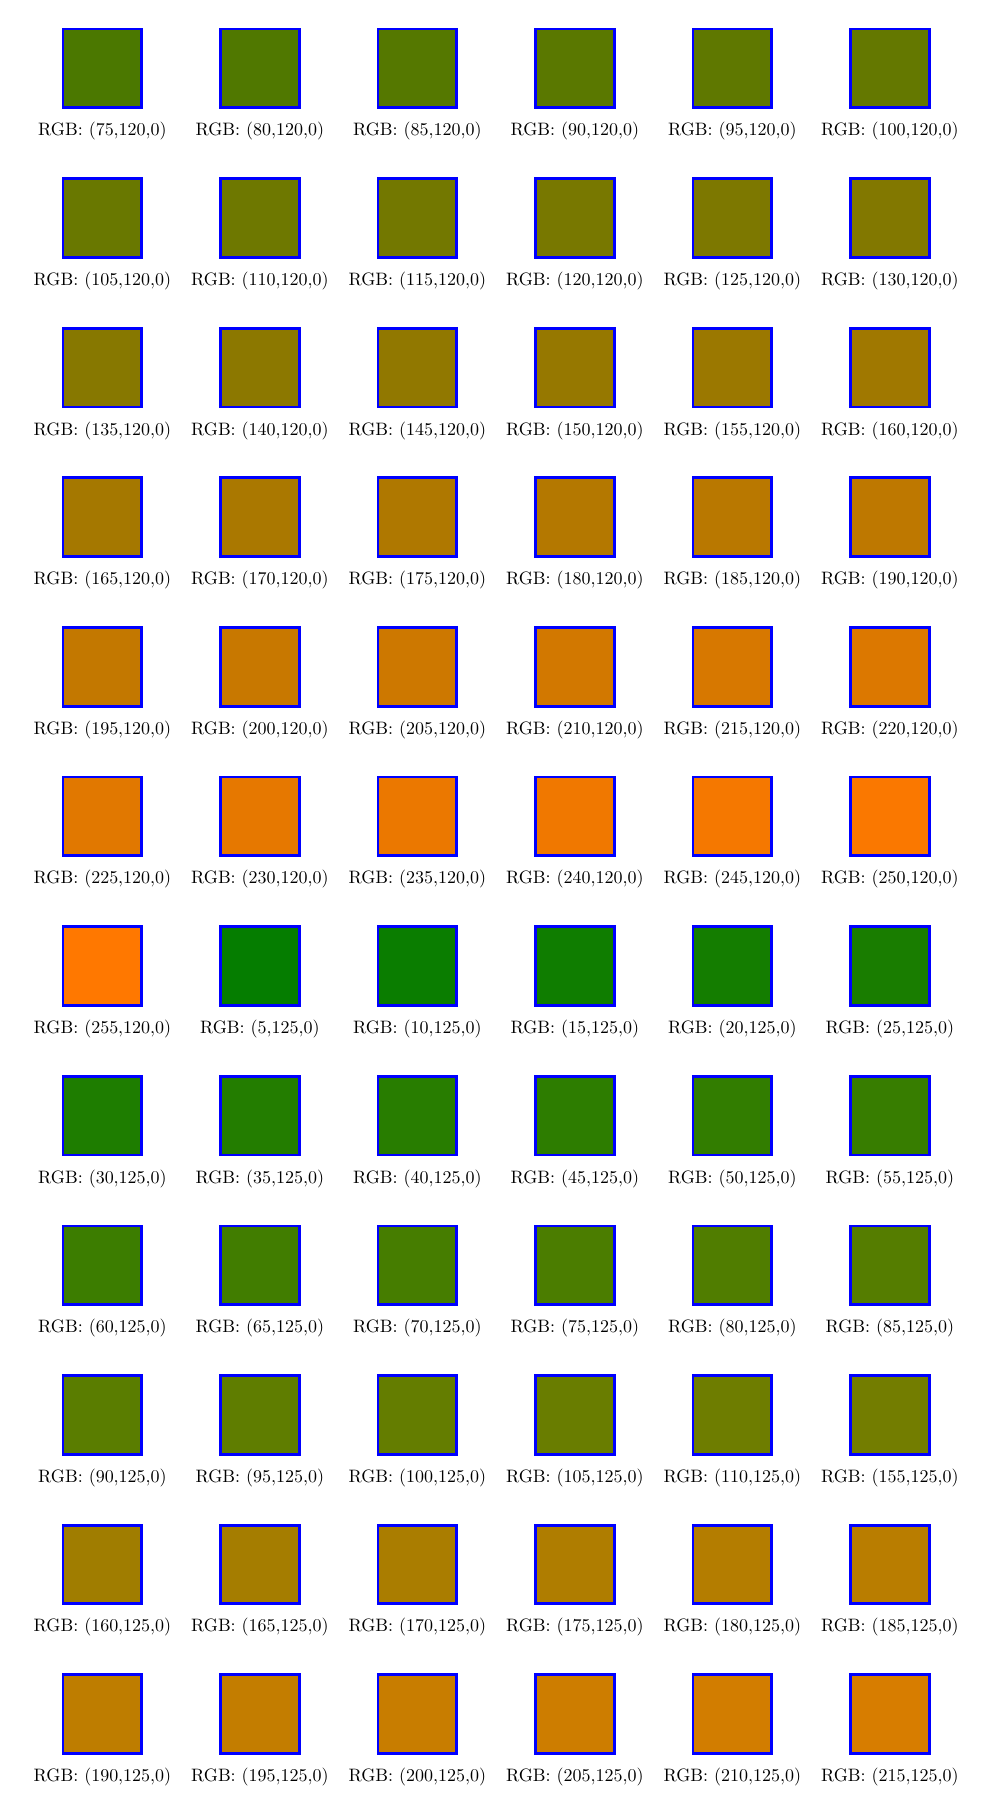
\begin{tikzpicture}

    \filldraw[draw=blue,line width=1,fill=colorR75G120B0]
    (0,0) rectangle (1,1);

    \node[scale=0.65] at (0.5,-0.3) {RGB: (75,120,0)};



    \begin{scope}[xshift=2cm]

      \filldraw[draw=blue,line width=1,fill=colorR80G120B0]
      (0,0) rectangle (1,1);

      \node[scale=0.65] at (0.5,-0.3) {RGB: (80,120,0)};

    \end{scope}



    \begin{scope}[xshift=4cm]

      \filldraw[draw=blue,line width=1,fill=colorR85G120B0]
      (0,0) rectangle (1,1);

      \node[scale=0.65] at (0.5,-0.3) {RGB: (85,120,0)};

    \end{scope}



    \begin{scope}[xshift=6cm]

      \filldraw[draw=blue,line width=1,fill=colorR90G120B0]
      (0,0) rectangle (1,1);

      \node[scale=0.65] at (0.5,-0.3) {RGB: (90,120,0)};

    \end{scope}



    \begin{scope}[xshift=8cm]

      \filldraw[draw=blue,line width=1,fill=colorR95G120B0]
      (0,0) rectangle (1,1);

      \node[scale=0.65] at (0.5,-0.3) {RGB: (95,120,0)};

    \end{scope}



    \begin{scope}[xshift=10cm]

      \filldraw[draw=blue,line width=1,fill=colorR100G120B0]
      (0,0) rectangle (1,1);

      \node[scale=0.65] at (0.5,-0.3) {RGB: (100,120,0)};

    \end{scope}







    \begin{scope}[yshift=-1.9cm]

      \filldraw[draw=blue,line width=1,fill=colorR105G120B0]
      (0,0) rectangle (1,1);

      \node[scale=0.65] at (0.5,-0.3) {RGB: (105,120,0)};

    \end{scope}



    \begin{scope}[xshift=2cm,yshift=-1.9cm]

      \filldraw[draw=blue,line width=1,fill=colorR110G120B0]
      (0,0) rectangle (1,1);

      \node[scale=0.65] at (0.5,-0.3) {RGB: (110,120,0)};

    \end{scope}



    \begin{scope}[xshift=4cm,yshift=-1.9cm]

      \filldraw[draw=blue,line width=1,fill=colorR115G120B0]
      (0,0) rectangle (1,1);

      \node[scale=0.65] at (0.5,-0.3) {RGB: (115,120,0)};

    \end{scope}



    \begin{scope}[xshift=6cm,yshift=-1.9cm]

      \filldraw[draw=blue,line width=1,fill=colorR120G120B0]
      (0,0) rectangle (1,1);

      \node[scale=0.65] at (0.5,-0.3) {RGB: (120,120,0)};

    \end{scope}



    \begin{scope}[xshift=8cm,yshift=-1.9cm]

      \filldraw[draw=blue,line width=1,fill=colorR125G120B0]
      (0,0) rectangle (1,1);

      \node[scale=0.65] at (0.5,-0.3) {RGB: (125,120,0)};

    \end{scope}



    \begin{scope}[xshift=10cm,yshift=-1.9cm]

      \filldraw[draw=blue,line width=1,fill=colorR130G120B0]
      (0,0) rectangle (1,1);

      \node[scale=0.65] at (0.5,-0.3) {RGB: (130,120,0)};

    \end{scope}







    \begin{scope}[yshift=-3.8cm]

      \filldraw[draw=blue,line width=1,fill=colorR135G120B0]
      (0,0) rectangle (1,1);

      \node[scale=0.65] at (0.5,-0.3) {RGB: (135,120,0)};

    \end{scope}



    \begin{scope}[xshift=2cm,yshift=-3.8cm]

      \filldraw[draw=blue,line width=1,fill=colorR140G120B0]
      (0,0) rectangle (1,1);

      \node[scale=0.65] at (0.5,-0.3) {RGB: (140,120,0)};

    \end{scope}



    \begin{scope}[xshift=4cm,yshift=-3.8cm]

      \filldraw[draw=blue,line width=1,fill=colorR145G120B0]
      (0,0) rectangle (1,1);

      \node[scale=0.65] at (0.5,-0.3) {RGB: (145,120,0)};

    \end{scope}



    \begin{scope}[xshift=6cm,yshift=-3.8cm]

      \filldraw[draw=blue,line width=1,fill=colorR150G120B0]
      (0,0) rectangle (1,1);

      \node[scale=0.65] at (0.5,-0.3) {RGB: (150,120,0)};

    \end{scope}



    \begin{scope}[xshift=8cm,yshift=-3.8cm]

      \filldraw[draw=blue,line width=1,fill=colorR155G120B0]
      (0,0) rectangle (1,1);

      \node[scale=0.65] at (0.5,-0.3) {RGB: (155,120,0)};

    \end{scope}



    \begin{scope}[xshift=10cm,yshift=-3.8cm]

      \filldraw[draw=blue,line width=1,fill=colorR160G120B0]
      (0,0) rectangle (1,1);

      \node[scale=0.65] at (0.5,-0.3) {RGB: (160,120,0)};

    \end{scope}







    \begin{scope}[yshift=-5.7cm]

      \filldraw[draw=blue,line width=1,fill=colorR165G120B0]
      (0,0) rectangle (1,1);

      \node[scale=0.65] at (0.5,-0.3) {RGB: (165,120,0)};

    \end{scope}



    \begin{scope}[xshift=2cm,yshift=-5.7cm]

      \filldraw[draw=blue,line width=1,fill=colorR170G120B0]
      (0,0) rectangle (1,1);

      \node[scale=0.65] at (0.5,-0.3) {RGB: (170,120,0)};

    \end{scope}



    \begin{scope}[xshift=4cm,yshift=-5.7cm]

      \filldraw[draw=blue,line width=1,fill=colorR175G120B0]
      (0,0) rectangle (1,1);

      \node[scale=0.65] at (0.5,-0.3) {RGB: (175,120,0)};

    \end{scope}



    \begin{scope}[xshift=6cm,yshift=-5.7cm]

      \filldraw[draw=blue,line width=1,fill=colorR180G120B0]
      (0,0) rectangle (1,1);

      \node[scale=0.65] at (0.5,-0.3) {RGB: (180,120,0)};

    \end{scope}



    \begin{scope}[xshift=8cm,yshift=-5.7cm]

      \filldraw[draw=blue,line width=1,fill=colorR185G120B0]
      (0,0) rectangle (1,1);

      \node[scale=0.65] at (0.5,-0.3) {RGB: (185,120,0)};

    \end{scope}



    \begin{scope}[xshift=10cm,yshift=-5.7cm]

      \filldraw[draw=blue,line width=1,fill=colorR190G120B0]
      (0,0) rectangle (1,1);

      \node[scale=0.65] at (0.5,-0.3) {RGB: (190,120,0)};

    \end{scope}







    \begin{scope}[yshift=-7.6cm]

      \filldraw[draw=blue,line width=1,fill=colorR195G120B0]
      (0,0) rectangle (1,1);

      \node[scale=0.65] at (0.5,-0.3) {RGB: (195,120,0)};

    \end{scope}



    \begin{scope}[xshift=2cm,yshift=-7.6cm]

      \filldraw[draw=blue,line width=1,fill=colorR200G120B0]
      (0,0) rectangle (1,1);

      \node[scale=0.65] at (0.5,-0.3) {RGB: (200,120,0)};

    \end{scope}



    \begin{scope}[xshift=4cm,yshift=-7.6cm]

      \filldraw[draw=blue,line width=1,fill=colorR205G120B0]
      (0,0) rectangle (1,1);

      \node[scale=0.65] at (0.5,-0.3) {RGB: (205,120,0)};

    \end{scope}



    \begin{scope}[xshift=6cm,yshift=-7.6cm]

      \filldraw[draw=blue,line width=1,fill=colorR210G120B0]
      (0,0) rectangle (1,1);

      \node[scale=0.65] at (0.5,-0.3) {RGB: (210,120,0)};

    \end{scope}



    \begin{scope}[xshift=8cm,yshift=-7.6cm]

      \filldraw[draw=blue,line width=1,fill=colorR215G120B0]
      (0,0) rectangle (1,1);

      \node[scale=0.65] at (0.5,-0.3) {RGB: (215,120,0)};

    \end{scope}



    \begin{scope}[xshift=10cm,yshift=-7.6cm]

      \filldraw[draw=blue,line width=1,fill=colorR220G120B0]
      (0,0) rectangle (1,1);

      \node[scale=0.65] at (0.5,-0.3) {RGB: (220,120,0)};

    \end{scope}







    \begin{scope}[yshift=-9.5cm]

      \filldraw[draw=blue,line width=1,fill=colorR225G120B0]
      (0,0) rectangle (1,1);

      \node[scale=0.65] at (0.5,-0.3) {RGB: (225,120,0)};

    \end{scope}



    \begin{scope}[xshift=2cm,yshift=-9.5cm]

      \filldraw[draw=blue,line width=1,fill=colorR230G120B0]
      (0,0) rectangle (1,1);

      \node[scale=0.65] at (0.5,-0.3) {RGB: (230,120,0)};

    \end{scope}



    \begin{scope}[xshift=4cm,yshift=-9.5cm]

      \filldraw[draw=blue,line width=1,fill=colorR235G120B0]
      (0,0) rectangle (1,1);

      \node[scale=0.65] at (0.5,-0.3) {RGB: (235,120,0)};

    \end{scope}



    \begin{scope}[xshift=6cm,yshift=-9.5cm]

      \filldraw[draw=blue,line width=1,fill=colorR240G120B0]
      (0,0) rectangle (1,1);

      \node[scale=0.65] at (0.5,-0.3) {RGB: (240,120,0)};

    \end{scope}



    \begin{scope}[xshift=8cm,yshift=-9.5cm]

      \filldraw[draw=blue,line width=1,fill=colorR245G120B0]
      (0,0) rectangle (1,1);

      \node[scale=0.65] at (0.5,-0.3) {RGB: (245,120,0)};

    \end{scope}



    \begin{scope}[xshift=10cm,yshift=-9.5cm]

      \filldraw[draw=blue,line width=1,fill=colorR250G120B0]
      (0,0) rectangle (1,1);

      \node[scale=0.65] at (0.5,-0.3) {RGB: (250,120,0)};

    \end{scope}







    \begin{scope}[yshift=-11.4cm]

      \filldraw[draw=blue,line width=1,fill=colorR255G120B0]
      (0,0) rectangle (1,1);

      \node[scale=0.65] at (0.5,-0.3) {RGB: (255,120,0)};

    \end{scope}



    \begin{scope}[xshift=2cm,yshift=-11.4cm]

      \filldraw[draw=blue,line width=1,fill=colorR5G125B0]
      (0,0) rectangle (1,1);

      \node[scale=0.65] at (0.5,-0.3) {RGB: (5,125,0)};

    \end{scope}



    \begin{scope}[xshift=4cm,yshift=-11.4cm]

      \filldraw[draw=blue,line width=1,fill=colorR10G125B0]
      (0,0) rectangle (1,1);

      \node[scale=0.65] at (0.5,-0.3) {RGB: (10,125,0)};

    \end{scope}



    \begin{scope}[xshift=6cm,yshift=-11.4cm]

      \filldraw[draw=blue,line width=1,fill=colorR15G125B0]
      (0,0) rectangle (1,1);

      \node[scale=0.65] at (0.5,-0.3) {RGB: (15,125,0)};

    \end{scope}



    \begin{scope}[xshift=8cm,yshift=-11.4cm]

      \filldraw[draw=blue,line width=1,fill=colorR20G125B0]
      (0,0) rectangle (1,1);

      \node[scale=0.65] at (0.5,-0.3) {RGB: (20,125,0)};

    \end{scope}



    \begin{scope}[xshift=10cm,yshift=-11.4cm]

      \filldraw[draw=blue,line width=1,fill=colorR25G125B0]
      (0,0) rectangle (1,1);

      \node[scale=0.65] at (0.5,-0.3) {RGB: (25,125,0)};

    \end{scope}







    \begin{scope}[yshift=-13.3cm]

      \filldraw[draw=blue,line width=1,fill=colorR30G125B0]
      (0,0) rectangle (1,1);

      \node[scale=0.65] at (0.5,-0.3) {RGB: (30,125,0)};

    \end{scope}



    \begin{scope}[xshift=2cm,yshift=-13.3cm]

      \filldraw[draw=blue,line width=1,fill=colorR35G125B0]
      (0,0) rectangle (1,1);

      \node[scale=0.65] at (0.5,-0.3) {RGB: (35,125,0)};

    \end{scope}



    \begin{scope}[xshift=4cm,yshift=-13.3cm]

      \filldraw[draw=blue,line width=1,fill=colorR40G125B0]
      (0,0) rectangle (1,1);

      \node[scale=0.65] at (0.5,-0.3) {RGB: (40,125,0)};

    \end{scope}



    \begin{scope}[xshift=6cm,yshift=-13.3cm]

      \filldraw[draw=blue,line width=1,fill=colorR45G125B0]
      (0,0) rectangle (1,1);

      \node[scale=0.65] at (0.5,-0.3) {RGB: (45,125,0)};

    \end{scope}



    \begin{scope}[xshift=8cm,yshift=-13.3cm]

      \filldraw[draw=blue,line width=1,fill=colorR50G125B0]
      (0,0) rectangle (1,1);

      \node[scale=0.65] at (0.5,-0.3) {RGB: (50,125,0)};

    \end{scope}



    \begin{scope}[xshift=10cm,yshift=-13.3cm]

      \filldraw[draw=blue,line width=1,fill=colorR55G125B0]
      (0,0) rectangle (1,1);

      \node[scale=0.65] at (0.5,-0.3) {RGB: (55,125,0)};

    \end{scope}







    \begin{scope}[yshift=-15.2cm]

      \filldraw[draw=blue,line width=1,fill=colorR60G125B0]
      (0,0) rectangle (1,1);

      \node[scale=0.65] at (0.5,-0.3) {RGB: (60,125,0)};

    \end{scope}



    \begin{scope}[xshift=2cm,yshift=-15.2cm]

      \filldraw[draw=blue,line width=1,fill=colorR65G125B0]
      (0,0) rectangle (1,1);

      \node[scale=0.65] at (0.5,-0.3) {RGB: (65,125,0)};

    \end{scope}



    \begin{scope}[xshift=4cm,yshift=-15.2cm]

      \filldraw[draw=blue,line width=1,fill=colorR70G125B0]
      (0,0) rectangle (1,1);

      \node[scale=0.65] at (0.5,-0.3) {RGB: (70,125,0)};

    \end{scope}



    \begin{scope}[xshift=6cm,yshift=-15.2cm]

      \filldraw[draw=blue,line width=1,fill=colorR75G125B0]
      (0,0) rectangle (1,1);

      \node[scale=0.65] at (0.5,-0.3) {RGB: (75,125,0)};

    \end{scope}



    \begin{scope}[xshift=8cm,yshift=-15.2cm]

      \filldraw[draw=blue,line width=1,fill=colorR80G125B0]
      (0,0) rectangle (1,1);

      \node[scale=0.65] at (0.5,-0.3) {RGB: (80,125,0)};

    \end{scope}



    \begin{scope}[xshift=10cm,yshift=-15.2cm]

      \filldraw[draw=blue,line width=1,fill=colorR85G125B0]
      (0,0) rectangle (1,1);

      \node[scale=0.65] at (0.5,-0.3) {RGB: (85,125,0)};

    \end{scope}







    \begin{scope}[yshift=-17.1cm]

      \filldraw[draw=blue,line width=1,fill=colorR90G125B0]
      (0,0) rectangle (1,1);

      \node[scale=0.65] at (0.5,-0.3) {RGB: (90,125,0)};

    \end{scope}



    \begin{scope}[xshift=2cm,yshift=-17.1cm]

      \filldraw[draw=blue,line width=1,fill=colorR95G125B0]
      (0,0) rectangle (1,1);

      \node[scale=0.65] at (0.5,-0.3) {RGB: (95,125,0)};

    \end{scope}



    \begin{scope}[xshift=4cm,yshift=-17.1cm]

      \filldraw[draw=blue,line width=1,fill=colorR100G125B0]
      (0,0) rectangle (1,1);

      \node[scale=0.65] at (0.5,-0.3) {RGB: (100,125,0)};

    \end{scope}



    \begin{scope}[xshift=6cm,yshift=-17.1cm]

      \filldraw[draw=blue,line width=1,fill=colorR105G125B0]
      (0,0) rectangle (1,1);

      \node[scale=0.65] at (0.5,-0.3) {RGB: (105,125,0)};

    \end{scope}



    \begin{scope}[xshift=8cm,yshift=-17.1cm]

      \filldraw[draw=blue,line width=1,fill=colorR110G125B0]
      (0,0) rectangle (1,1);

      \node[scale=0.65] at (0.5,-0.3) {RGB: (110,125,0)};

    \end{scope}



    \begin{scope}[xshift=10cm,yshift=-17.1cm]

      \filldraw[draw=blue,line width=1,fill=colorR115G125B0]
      (0,0) rectangle (1,1);

      \node[scale=0.65] at (0.5,-0.3) {RGB: (155,125,0)};

    \end{scope}







    \begin{scope}[yshift=-19cm]

      \filldraw[draw=blue,line width=1,fill=colorR160G125B0]
      (0,0) rectangle (1,1);

      \node[scale=0.65] at (0.5,-0.3) {RGB: (160,125,0)};

    \end{scope}



    \begin{scope}[xshift=2cm,yshift=-19cm]

      \filldraw[draw=blue,line width=1,fill=colorR165G125B0]
      (0,0) rectangle (1,1);

      \node[scale=0.65] at (0.5,-0.3) {RGB: (165,125,0)};

    \end{scope}



    \begin{scope}[xshift=4cm,yshift=-19cm]

      \filldraw[draw=blue,line width=1,fill=colorR170G125B0]
      (0,0) rectangle (1,1);

      \node[scale=0.65] at (0.5,-0.3) {RGB: (170,125,0)};

    \end{scope}



    \begin{scope}[xshift=6cm,yshift=-19cm]

      \filldraw[draw=blue,line width=1,fill=colorR175G125B0]
      (0,0) rectangle (1,1);

      \node[scale=0.65] at (0.5,-0.3) {RGB: (175,125,0)};

    \end{scope}



    \begin{scope}[xshift=8cm,yshift=-19cm]

      \filldraw[draw=blue,line width=1,fill=colorR180G125B0]
      (0,0) rectangle (1,1);

      \node[scale=0.65] at (0.5,-0.3) {RGB: (180,125,0)};

    \end{scope}



    \begin{scope}[xshift=10cm,yshift=-19cm]

      \filldraw[draw=blue,line width=1,fill=colorR185G125B0]
      (0,0) rectangle (1,1);

      \node[scale=0.65] at (0.5,-0.3) {RGB: (185,125,0)};

    \end{scope}







    \begin{scope}[yshift=-20.9cm]

      \filldraw[draw=blue,line width=1,fill=colorR190G125B0]
      (0,0) rectangle (1,1);

      \node[scale=0.65] at (0.5,-0.3) {RGB: (190,125,0)};

    \end{scope}



    \begin{scope}[xshift=2cm,yshift=-20.9cm]

      \filldraw[draw=blue,line width=1,fill=colorR195G125B0]
      (0,0) rectangle (1,1);

      \node[scale=0.65] at (0.5,-0.3) {RGB: (195,125,0)};

    \end{scope}



    \begin{scope}[xshift=4cm,yshift=-20.9cm]

      \filldraw[draw=blue,line width=1,fill=colorR200G125B0]
      (0,0) rectangle (1,1);

      \node[scale=0.65] at (0.5,-0.3) {RGB: (200,125,0)};

    \end{scope}



    \begin{scope}[xshift=6cm,yshift=-20.9cm]

      \filldraw[draw=blue,line width=1,fill=colorR205G125B0]
      (0,0) rectangle (1,1);

      \node[scale=0.65] at (0.5,-0.3) {RGB: (205,125,0)};

    \end{scope}



    \begin{scope}[xshift=8cm,yshift=-20.9cm]

      \filldraw[draw=blue,line width=1,fill=colorR210G125B0]
      (0,0) rectangle (1,1);

      \node[scale=0.65] at (0.5,-0.3) {RGB: (210,125,0)};

    \end{scope}



    \begin{scope}[xshift=10cm,yshift=-20.9cm]

      \filldraw[draw=blue,line width=1,fill=colorR215G125B0]
      (0,0) rectangle (1,1);

      \node[scale=0.65] at (0.5,-0.3) {RGB: (215,125,0)};

    \end{scope}

  \end{tikzpicture}

  \caption{Mixed colors in~RGB system: $(75,120,0)$--$(255,120,0)$,
    $(5,125,0)$--$(215,125,0)$}



  \label{fig:Mixed-colors-Part-09}

\end{figure}
% ##################





% ##################
\begin{figure}

  \centering


  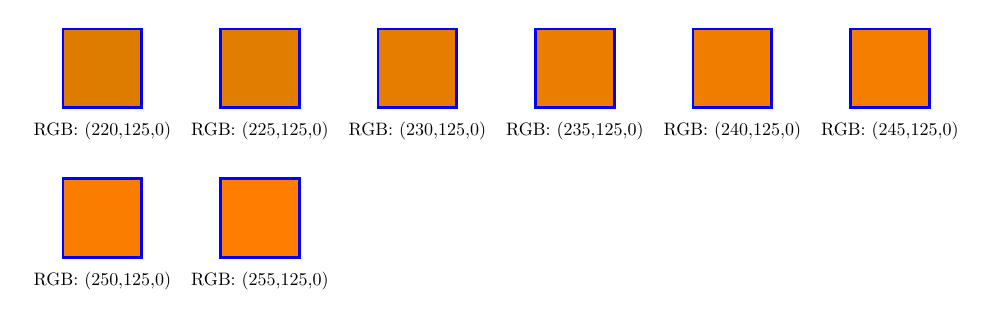
\begin{tikzpicture}

    \filldraw[draw=blue,line width=1,fill=colorR220G125B0]
    (0,0) rectangle (1,1);

    \node[scale=0.65] at (0.5,-0.3) {RGB: (220,125,0)};



    \begin{scope}[xshift=2cm]

      \filldraw[draw=blue,line width=1,fill=colorR225G125B0]
      (0,0) rectangle (1,1);

      \node[scale=0.65] at (0.5,-0.3) {RGB: (225,125,0)};

    \end{scope}



    \begin{scope}[xshift=4cm]

      \filldraw[draw=blue,line width=1,fill=colorR230G125B0]
      (0,0) rectangle (1,1);

      \node[scale=0.65] at (0.5,-0.3) {RGB: (230,125,0)};

    \end{scope}



    \begin{scope}[xshift=6cm]

      \filldraw[draw=blue,line width=1,fill=colorR235G125B0]
      (0,0) rectangle (1,1);

      \node[scale=0.65] at (0.5,-0.3) {RGB: (235,125,0)};

    \end{scope}



    \begin{scope}[xshift=8cm]

      \filldraw[draw=blue,line width=1,fill=colorR240G125B0]
      (0,0) rectangle (1,1);

      \node[scale=0.65] at (0.5,-0.3) {RGB: (240,125,0)};

    \end{scope}



    \begin{scope}[xshift=10cm]

      \filldraw[draw=blue,line width=1,fill=colorR245G125B0]
      (0,0) rectangle (1,1);

      \node[scale=0.65] at (0.5,-0.3) {RGB: (245,125,0)};

    \end{scope}







    \begin{scope}[yshift=-1.9cm]

      \filldraw[draw=blue,line width=1,fill=colorR250G125B0]
      (0,0) rectangle (1,1);

      \node[scale=0.65] at (0.5,-0.3) {RGB: (250,125,0)};

    \end{scope}



    \begin{scope}[xshift=2cm,yshift=-1.9cm]

      \filldraw[draw=blue,line width=1,fill=colorR255G125B0]
      (0,0) rectangle (1,1);

      \node[scale=0.65] at (0.5,-0.3) {RGB: (255,125,0)};

    \end{scope}

  \end{tikzpicture}

  \caption{Mixed colors in~RGB system: $(225,125,0)$--$(255,125,0)$}



  \label{fig:Mixed-colors-Part-10}

\end{figure}
% ##################










% ####################################################################
% ####################################################################
% Bibliography

% \printbibliography





% ############################
% End of the document

\end{document}
